% \documentclass{article}
% \usepackage{natbib} 
\documentclass[11pt]{article}
\usepackage[review]{acl}
\usepackage{times}


\usepackage[utf8]{inputenc} % allow utf-8 input
\usepackage[T1]{fontenc}    % use 8-bit T1 fonts
\usepackage{hyperref}       % hyperlinks
\usepackage{url}            % simple URL typesetting
\usepackage{booktabs}       % professional-quality tables
\usepackage{amsfonts}       % blackboard math symbols
\usepackage{nicefrac}       % compact symbols for 1/2, etc.
\usepackage{microtype}      % microtypography
\usepackage{xcolor}         % colors
\usepackage{tabularx}
\usepackage{enumitem}
\usepackage{float}
\usepackage{placeins}
\usepackage{needspace}
\usepackage{listings}
\usepackage{xcolor}
\usepackage{tcolorbox}
\tcbuselibrary{breakable}
\usepackage{fvextra}
\usepackage{xspace}
\usepackage{enumitem}
\usepackage{amsmath}
\usepackage{pifont}
\usepackage{colortbl}
\usepackage{makecell}
\usepackage{caption}  % for \captionof in minipage
\usepackage{wrapfig}  % for wrap figures/tables
\usepackage{marvosym}
\usepackage{tikz}
% 引入插图宏包（如果你还没加的话）
\usepackage{graphicx}

% benchmark comparison table colors & commands
\definecolor{BenchHeaderBg}{RGB}{40, 100, 175}
\definecolor{BenchAltRow}{RGB}{230, 240, 252}
\definecolor{BenchOursRow}{RGB}{195, 240, 205}

\newcommand{\cmark}{\textcolor{green!60!black}{\ding{51}}}
\newcommand{\xmark}{\textcolor{red!70!black}{\ding{55}}}
\newcommand{\pmark}{\textcolor{orange!80!black}{\textbf{\textasciitilde}}}
\newcommand{\bhead}[1]{\textcolor{white}{\textbf{\small #1}}}

\newcommand{\todoc}[2]{{\textcolor{#1}{\textbf{[#2]}}}}
\newcommand{\todo}[1]{\todoblue{#1}} % 默认使用蓝色 todo

\newcommand{\todoblue}[1]{\todoc{blue}{\textbf{#1}}}
\newcommand{\todored}[1]{\todoc{red}{\textbf{#1}}}
\newcommand{\todoorange}[1]{\todoc{orange}{\textbf{#1}}}
\newcommand{\todopurple}[1]{\todoc{pruple}{\textbf{#1}}}

\newcommand{\peng}[1]{\todoblue{peng: #1}}
\newcommand{\zhang}[1]{\todoblue{zhang: #1}}
\newcommand{\shi}[1]{\todoorange{shi: #1}}
\newcommand{\gu}[1]{\todored{gu: #1}}

\newcommand{\feng}[1]{\todopurple{Feng: #1}}


\newcommand{\ourbench}[0]{\textsc{HEART-Bench}\xspace}
% \newcommand{\hficon}{%
%   \raisebox{-0.2\height}{
\includegraphics[height=1em]{figures/hf-logo.pdf}}%
% }

\title{\ourbench: Do LLMs Make Persona-Consistent Decisions?}

\author{}

\begin{document}


\maketitle

\begin{abstract}
While LLMs have demonstrated strong task-oriented capabilities, their ability to make persona-consistent decisions grounded in long-term memory remains underexplored. We introduce \ourbench, a benchmark of psychology-informed, memory-grounded persona consistency in controlled synthetic settings. \ourbench defines 11 characters using Big Five--anchored profiles and value-based specifications, assigns each character 1,000 synthetic autobiographical memories, and evaluates them across 64 DIAMONDS-guided decision scenarios. Each character--scenario pair is associated with a response that the character is expected to have under the specific scenario. Three domain experts independently compare anonymized candidates, and a senior expert selects, revises, or rewrites the final reference when needed. This process yields 673 multiple-choice questions in which a model selects the option judged most consistent with the predefined character and its history. A separate expert panel audits 176 final items, all of which receive majority support for the existing key. We evaluate 12 LLMs under a No-Retrieval baseline and three memory-augmented settings: Naive-RAG, Mem0, and PersonaDB. The strongest configuration, Gemini-3.1-Pro with Naive-RAG, reaches 63.3\% accuracy, while most models remain below 40\%. These results show substantial difficulty in selecting expert-adjudicated responses consistent with predefined characters and their memories.
\end{abstract}

\begin{figure}[ht]
\centering
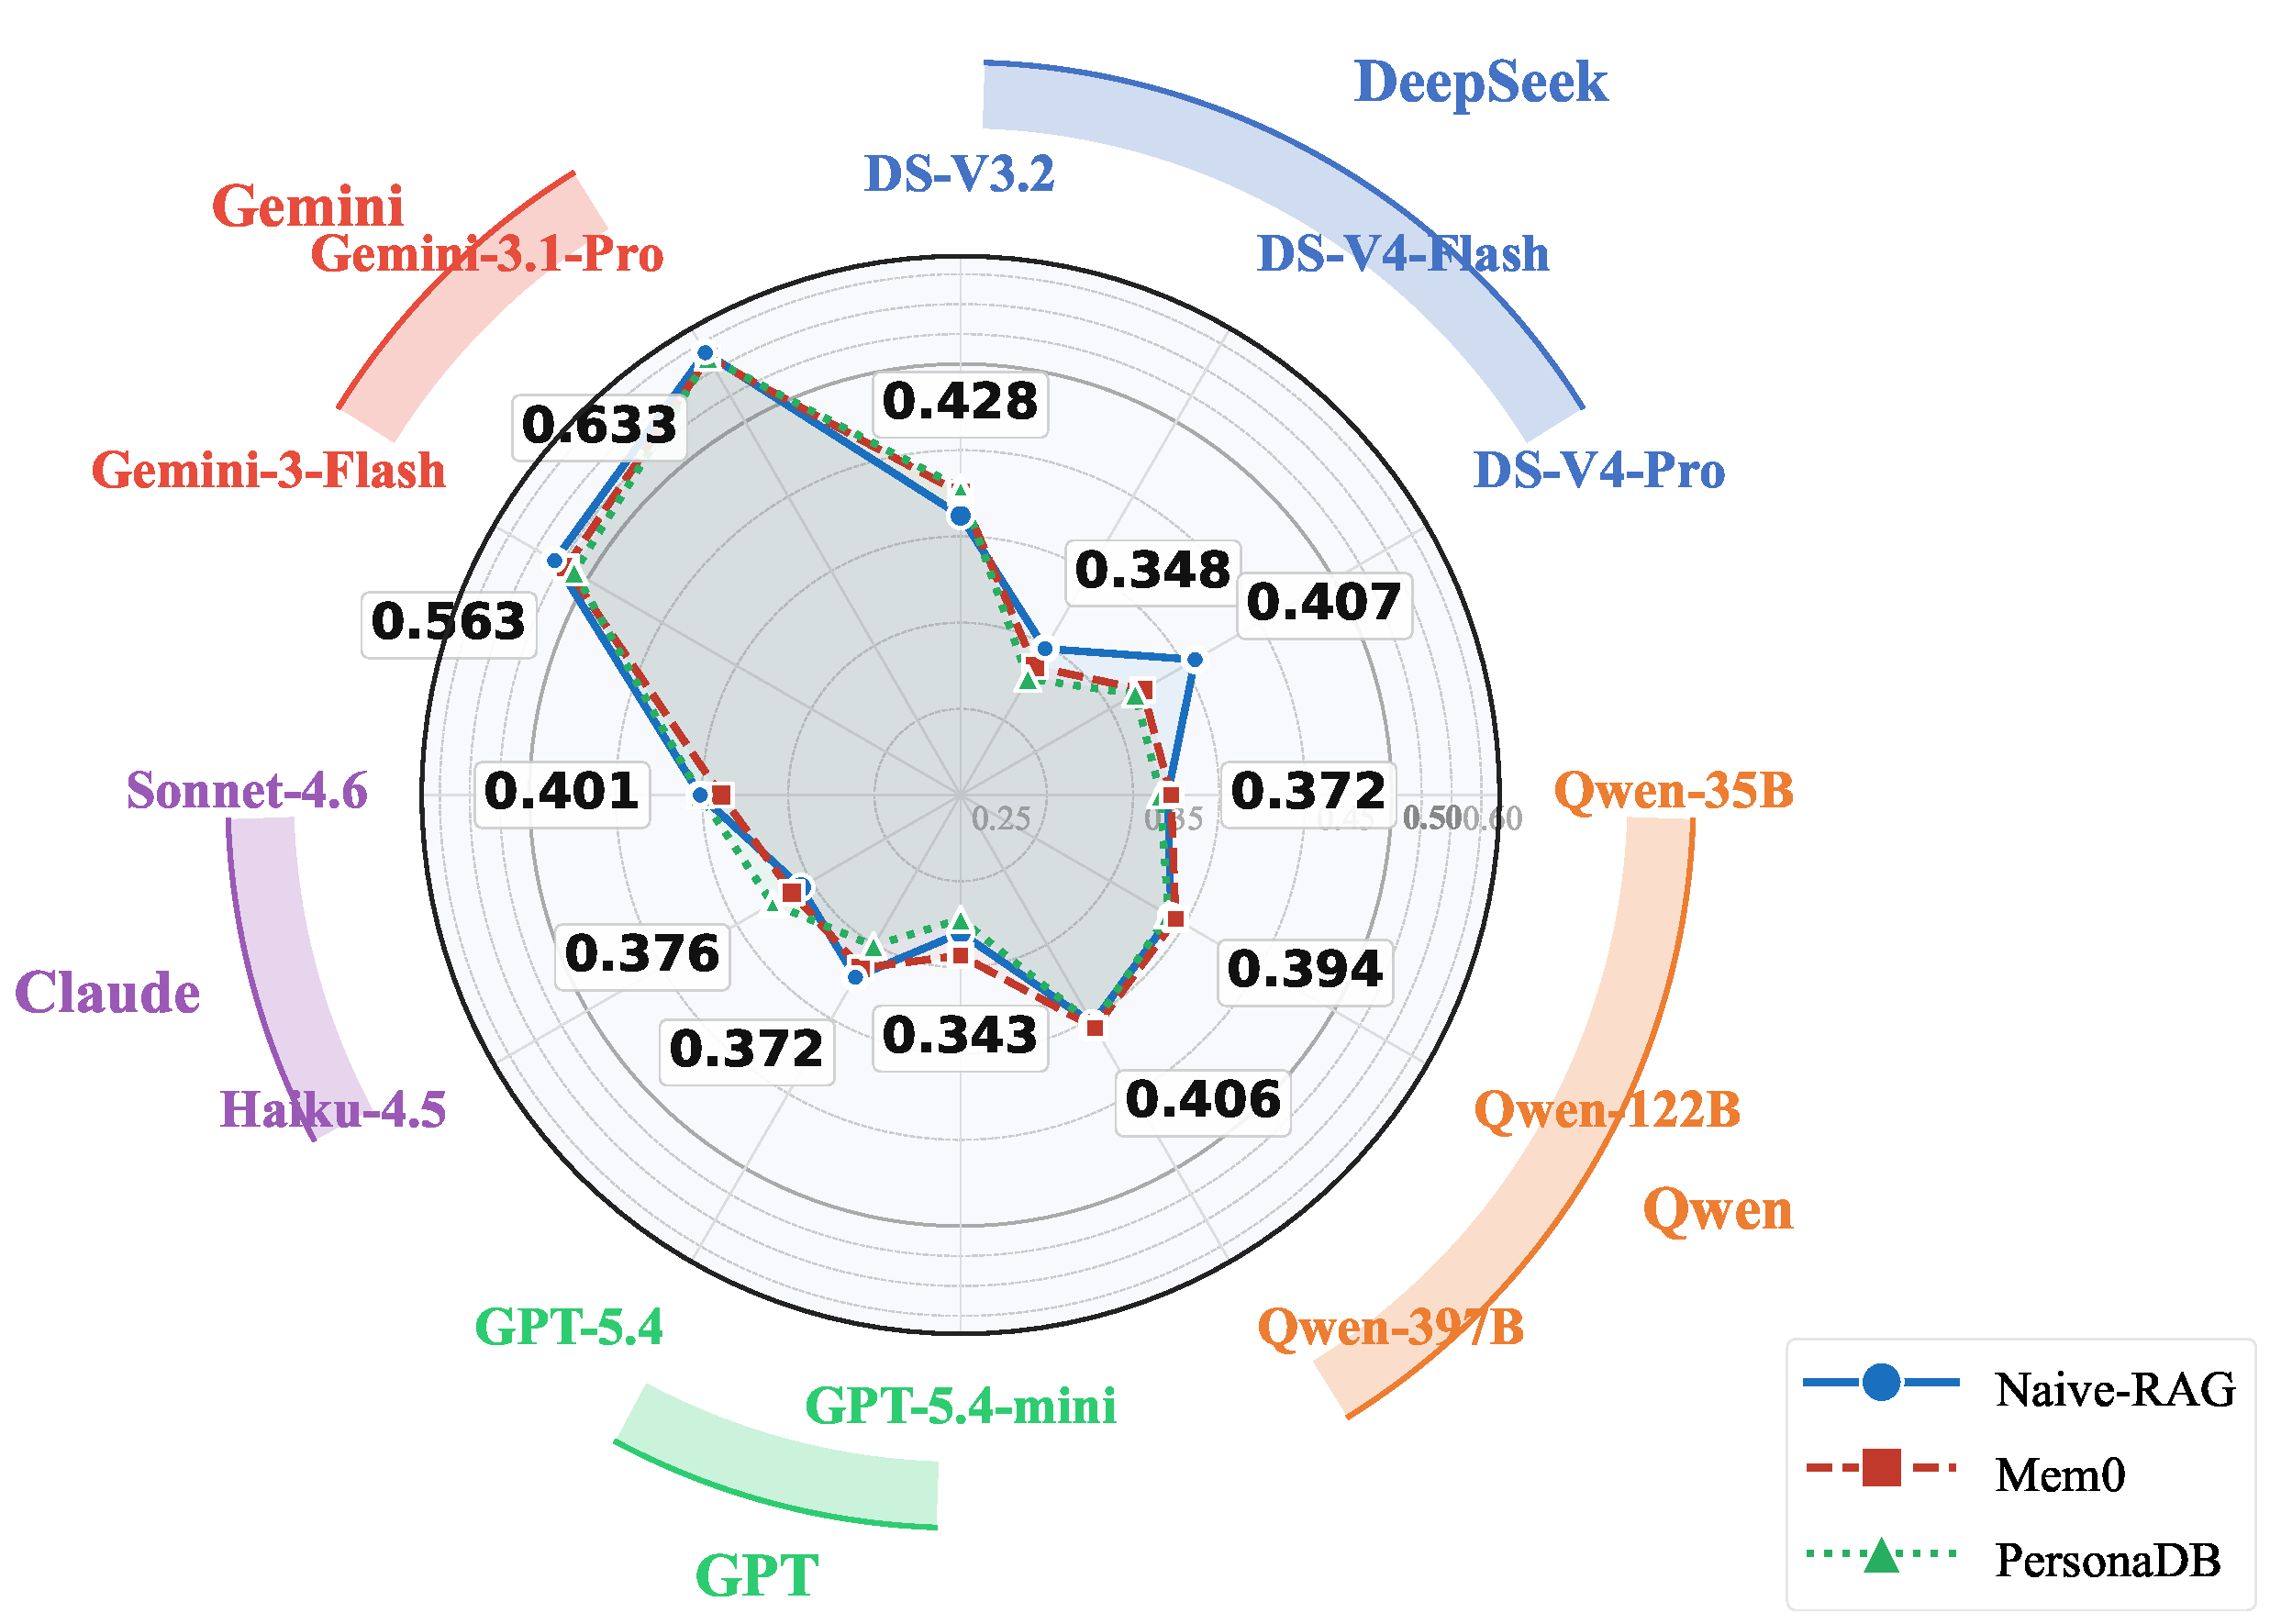
\includegraphics[width=\linewidth]{figures/radar_3configs_v2.pdf}
\caption{Accuracy for all 12 models, shown separately for the three memory-augmented settings.}
\label{fig:radar_configs}
\vspace{-15pt}
\end{figure}

\section{Introduction}
\label{sec:Introduction}

Large language models (LLMs) have achieved substantial progress in planning, reasoning, and action~\cite{anthropic2026claudeopus47,openai2026gpt55,google2026gemini31pro}. As LLM agents are increasingly deployed in entertainment~\cite{chen2024persona,tseng2024two}, AI companionship~\cite{maples2024loneliness,phang2025investigating}, and persona-cloning systems~\cite{wei2025ai,lee2026creating}, users increasingly expect persistent and personalized behavior. These applications require more than conversational fluency and memory recall: a system should use a character's traits, values, and prior experiences consistently when choosing how to respond. Existing evaluations, however, primarily target dialogue, explicit reasoning, or memory retrieval. This leaves a narrower but important question unresolved: \emph{Given a predefined character, its history, and a scenario, can an LLM select a persona-consistent response?}
% As LLMs become increasingly integrated into entertainment \cite{tseng2024two}, social networking \cite{?}, and emotional companionship \cite{chen2024persona}, user expectations for anthropomorphic AI agents have evolved from merely task assistant to providing long-term emotional companionship. When these capabilities are realized and effectively synergized, AI agents may acquire the foundational prerequisites for more advanced forms of affective intelligence---a critical milestone in the pursuit of higher artificial Emotional Intelligence (EI) \cite{?}.
\begin{table*}[t]
\centering
\footnotesize
\caption{Comparison of \ourbench with related benchmarks across six dimensions (see Appendix~\ref{app:benchmark_dims} for dimension definitions).
\vspace{-5pt}
\cmark~yes;~~\xmark~no;~~\pmark~partial.}
\label{tab:benchmark_comparison}
\resizebox{\textwidth}{!}{
\begin{tabular}{lcccccc}
\toprule
\textbf{Benchmark} &
\textbf{Big Five-grounded} &
\textbf{\makecell{Age-defined\\life-stage coverage}} &
\textbf{Episodic memory} &
\textbf{Scenario eval.} &
\textbf{Expert annot.} &
\textbf{\makecell{Persona-consistent\\decision}} \\
\midrule
%KnowMeBench~\cite{wu2026knowme}          & \xmark & \pmark & \pmark & \pmark & \cmark & \xmark \\
\rowcolor{BenchAltRow}
CharacterEval~\cite{tu2024charactereval} & \xmark & \xmark & \xmark & \cmark & \pmark & \xmark \\
PersonaHub~\cite{ge2024scaling}       & \xmark & \xmark & \xmark & \cmark & \xmark & \xmark \\
\rowcolor{BenchAltRow}
LoCoMo~\cite{maharana2024evaluating}     & \xmark & \xmark & \cmark & \cmark & \xmark & \xmark \\
%LongMemEval~\cite{wu2024longmemeval}     & \xmark & \xmark & \cmark & \cmark & \xmark & \xmark \\
CloneMem~\cite{hu2026clonemem}           & \cmark & \pmark & \cmark & \xmark & \xmark & \xmark \\
\rowcolor{BenchAltRow}
%RealMem~\cite{bian2026realmem}           & \xmark & \pmark & \cmark & \cmark & \xmark & \xmark \\
PersonaLens~\cite{zhao2025personalens}   & \xmark & \xmark & \pmark & \cmark & \pmark & \xmark \\
PersonaMem~\cite{jiang2025personamem}    & \xmark & \xmark & \pmark & \cmark & \xmark & \xmark \\
\midrule
\rowcolor{BenchOursRow}
\textbf{\ourbench}       & \cmark & \cmark & \cmark & \cmark & \cmark & \cmark \\
\bottomrule
\end{tabular}
}
\vspace{-10pt}
\end{table*}

To address this gap, we introduce \ourbench, a controlled benchmark for evaluating memory-grounded persona consistency. \ourbench constructs 11 synthetic characters grounded in Big Five--anchored profiles, each associated with 1,000 structured synthetic autobiographical memories~\cite{singer1995seeing} organized into eight age-defined life-stage bins informed by developmental theories. We further design 64 decision scenarios guided by the DIAMONDS framework~\cite{rauthmann2014diamonds}. Each character--scenario pair is associated with a response that the character is expected to have under the specific scenario. To label ground truth responses, three domain experts independently compare candidate responses, and a senior expert handles every case not unanimously accepted as-is by selecting, revising, rewriting, or discarding the response. The adjudicated character response becomes the keyed reference, while responses associated with other characters in the same scenario provide distractor candidates. This process yields 673 multiple-choice questions; the memory-augmented settings test whether models can use relevant synthetic memories to identify the keyed response. Table~\ref{tab:benchmark_comparison} situates \ourbench relative to representative persona and memory benchmarks across six design dimensions.

%Throughout this paper, \emph{psychology-informed} describes the theoretical frameworks used to construct the benchmark; it does not imply that the synthetic characters instantiate human psychological processes. We operationalize \emph{persona consistency} as agreement between a model's selected option and an expert-adjudicated reference response conditioned on a predefined synthetic character profile, history, and scenario. Accordingly, \ourbench assesses consistency within this controlled construction rather than human likeness, genuine emotion, or predictive validity for real human behavior.



% The rapid advancement of Large Language Models (LLMs) has driven remarkable breakthroughs across numerous domains. However, existing research predominantly concentrates on task-oriented accuracy and conversational reasoning capabilities, rarely treating AI agents as complete human personalities where emotional dimensions hold equal importance. This raises an open question:\textcolor{blue}{ \emph{Do LLM agents exhibit human-like psychological characteristics, such as emotions and inherent values?}} This question sounds highly forward-looking, yet answering it has profound implications: As LLMs become increasingly integrated into entertainment, social networking, and emotional companionship, user expectations for anthropomorphic AI agents have evolved from simply "conversing like a human" to providing "long-term, memory-grounded emotional companionship." When these capabilities are fully realized and effectively synergized, AI agents will possess the foundational prerequisites for generating "human-like consciousness"---a critical milestone in the pursuit of higher artificial Emotional Intelligence (EI).

% Despite these evolving expectations, the current landscape of evaluation frameworks remains heavily constrained. Existing benchmarks primarily measure short- and long-term conversational context, explicit reasoning, memory recall, and end-to-end question-answering accuracy. While these efforts establish a foundational assessment framework for cognitive capabilities, merely advancing "conversation" and "memory" is insufficient. A pervasive lack of genuine "human touch" and empathy remains a significant bottleneck during long-term human-AI interactions. In the specific domain of evaluating the human-like psychology of AI agents, there is currently a complete void of standardized evaluation frameworks.

% To bridge this gap, we introduce \ourbench, a novel benchmark specifically designed to quantify the "human-like psychology of AI Agents." Our benchmark aims to facilitate the development of ``high-EI'' AI agents and significantly enhance the user experience in human-AI interactions.
% Specifically, our benchmark simulates 20 diverse human characters. Each character is grounded in a foundational five-dimensional personality framework (e.g., the Big Five personality traits) and is intricately associated with 1,000 memory episodes spanning distinct life stages. To rigorously evaluate the psychological manifestations of LLMs, we designed 50 evaluation scenarios woven into these key life milestones. During the evaluation process, the models are subjected to emotion-eliciting queries, requiring the LLM to reason over the characters' prior memory up to that age and infer the appropriate behavioral decision. 

%Our benchmark involves XXXX characters and XXXX scenarios, each is structured, psychologically informed. \gu{Give an overall description of the benchmark}. We constructs each \gu{Add description about characters} scenario using a hierarchical schema that explicitly models developmental stages, contextual environments, emotional dynamics, and decision-critical events. In particular, we incorporate psychological dimensions inspired by the DIAMONDS framework\cite{} in psychology to characterize situational structure and intensity, enabling fine-grained control over cognitive and emotional demands.

%Each scenario simulates a realistic interaction loop in which an agent must interpret contextual information, integrate long-term memory, and make value-consistent decisions under uncertainty. This design allows us to move beyond surface-level recall tasks toward evaluating whether agents can maintain coherent identity, adapt to evolving contexts, and exhibit consistent value-oriented behavior over time.

We evaluate 12 LLMs from the GPT, Claude, Gemini, DeepSeek, and Qwen families under a No-Retrieval baseline and three memory-augmented settings: Naive-RAG~\cite{lewis2020retrieval}, Mem0~\cite{chhikara2025mem0}, and PersonaDB~\cite{sun2025persona}. The strongest configuration, Gemini-3.1-Pro with Naive-RAG, reaches 63.3\% accuracy, while most models remain below 40\%. Within this controlled benchmark, the evaluated models therefore show limited ability to use encoded character and memory cues to select the expert-adjudicated response.


We summarize our contributions as follows:
\begin{itemize}[leftmargin=2em]
    \item We introduce a controlled benchmark comprising 11 psychology-informed synthetic characters, 11,000 synthetic autobiographical memories, 64 decision scenarios, and 673 expert-adjudicated MCQs.
    \item We operationalize memory-grounded persona consistency as agreement with an expert-adjudicated reference response conditioned on a predefined character, history, and scenario, and independently audit 176 items for reference-label reliability.
    \item We evaluate 12 LLMs across No-Retrieval and three memory-augmented settings, quantifying their ability to use encoded character and memory cues within this controlled synthetic setting.
\end{itemize}


% \begin{table}[t]
% \centering
% \small
% \caption{Comparison of \ourbench with related benchmarks across key dimensions.
% \cmark~yes;~~\xmark~no;~~\pmark~partial.
% \emph{Lifespan coverage}: explicit multi-stage developmental design (e.g., childhood, adolescence, adulthood) grounded in developmental psychology---multi-session dialogue time spans do not qualify.}
% \label{tab:benchmark_comparison}
% \begin{tabular}{lccccc}
% \toprule
% \textbf{Benchmark} &
% \textbf{\makecell{Big-Five\\grounded}} &
% \textbf{\makecell{Lifespan\\coverage}} &
% \textbf{\makecell{Episodic\\memory}} &
% \textbf{\makecell{Scenario\\eval.}} &
% \textbf{\makecell{Expert\\annot.}} \\

\begin{figure*}[t]
    \centering
    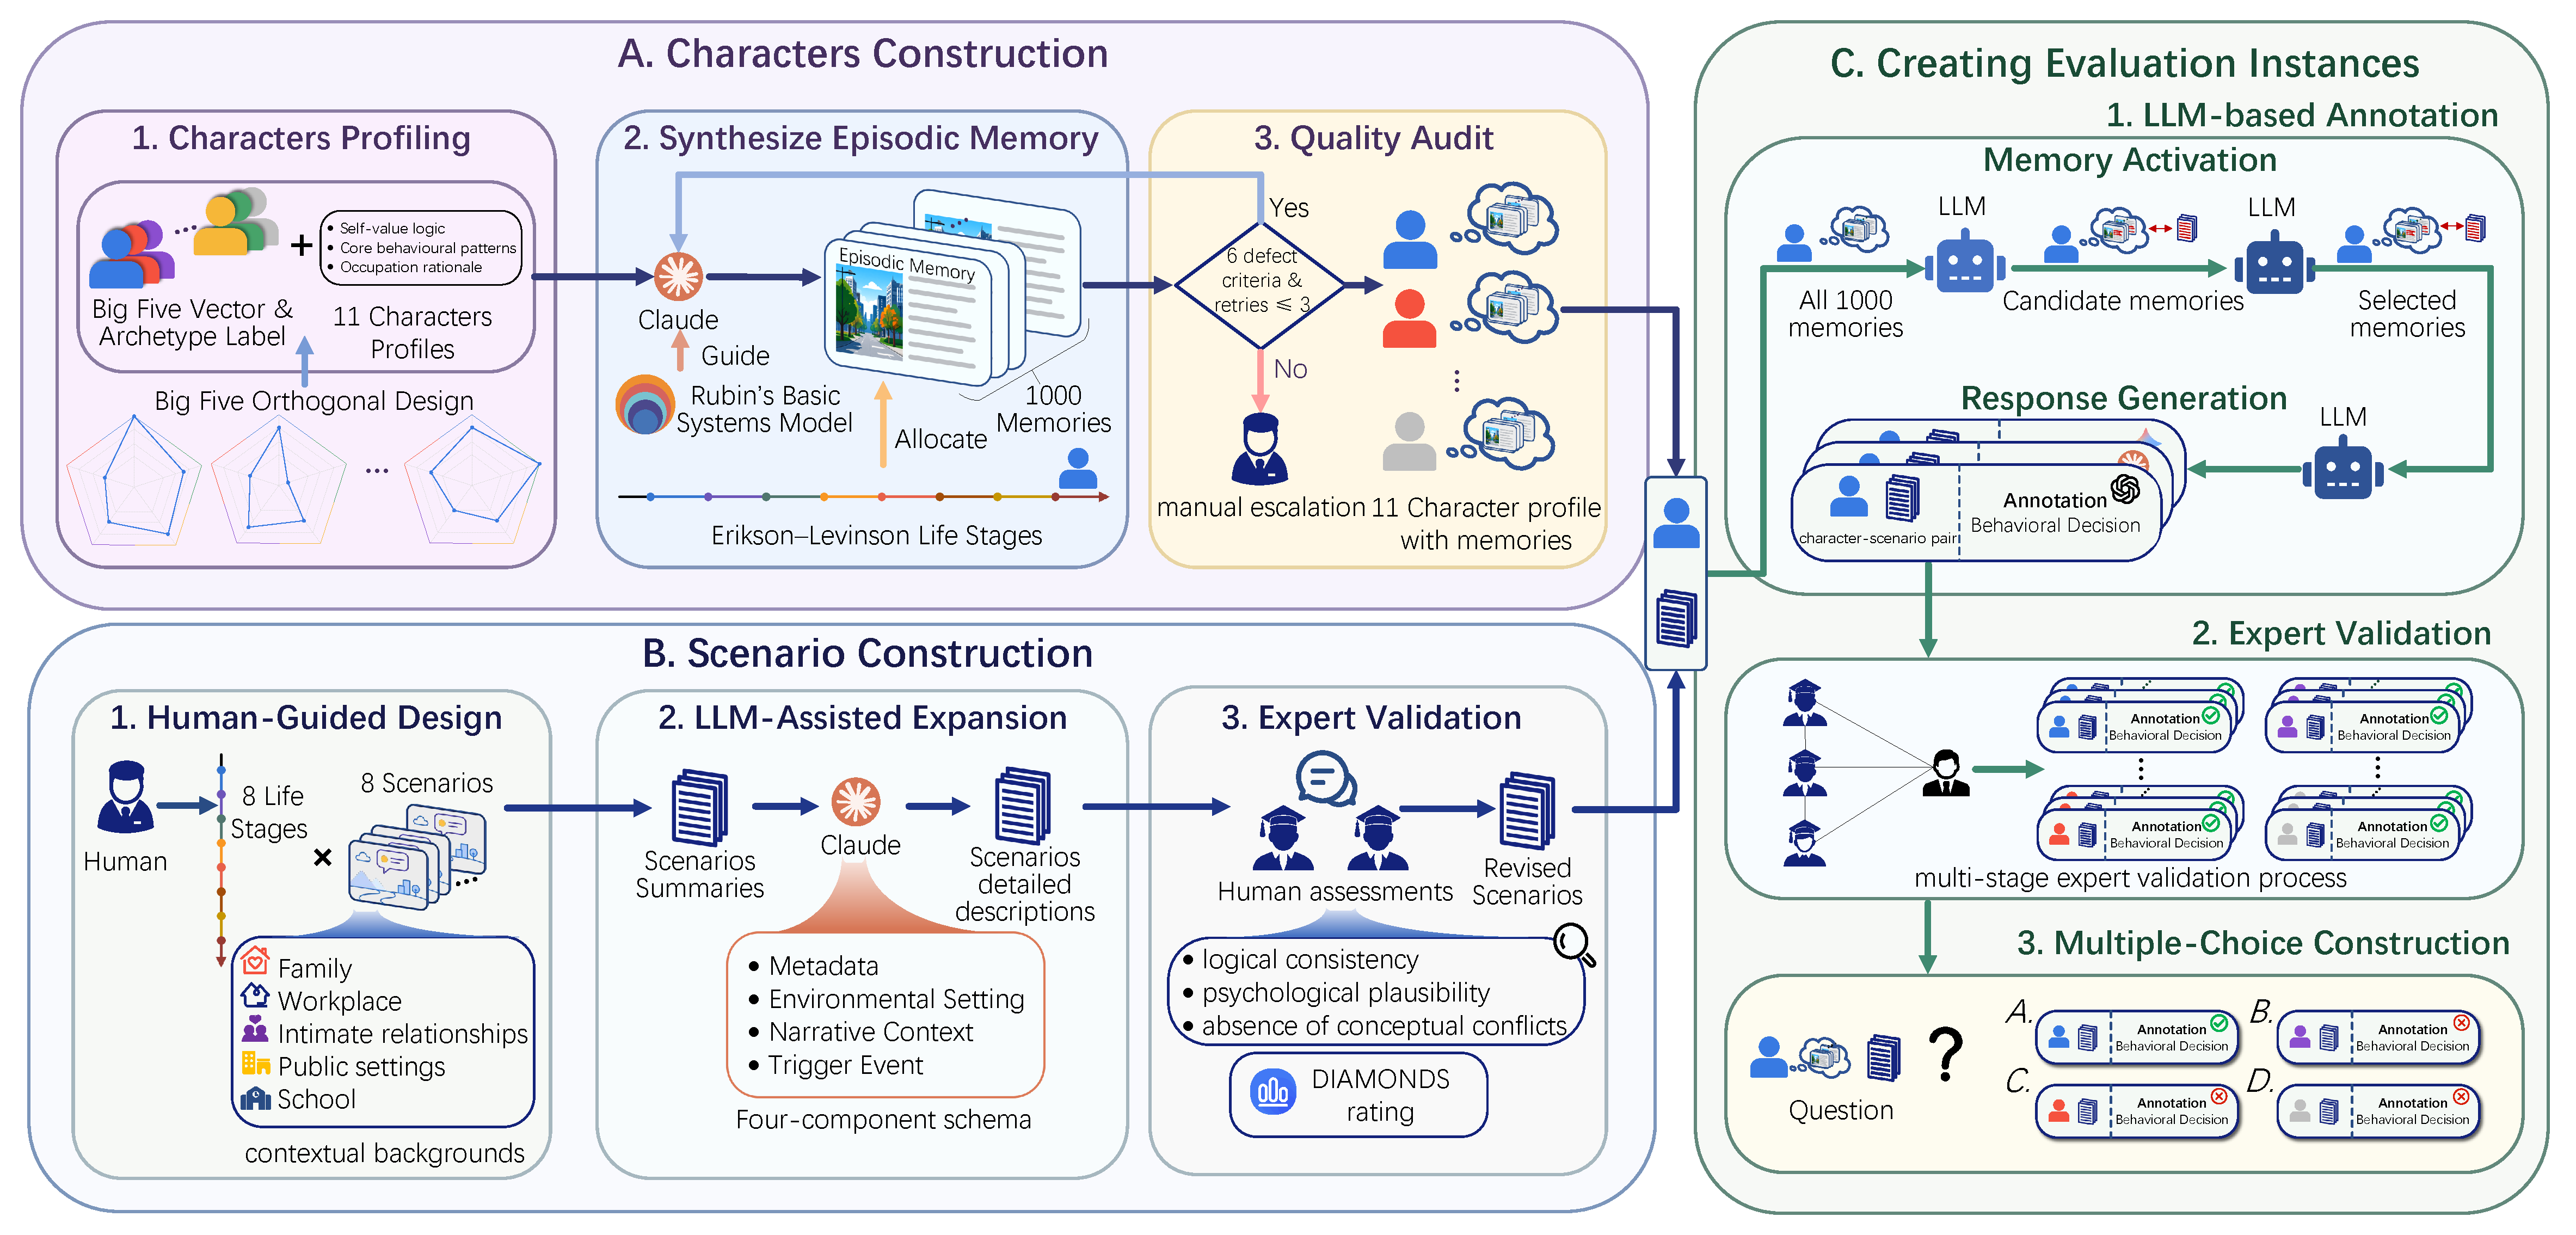
\includegraphics[width=1\linewidth]{figures/pipeline_v4.pdf}
    \caption{The pipeline has four stages: character construction, scenario construction, expert review and adjudication of reference responses, and conversion into MCQ format for model evaluation.}
    \label{fig:pipeline}
    \vspace{-10pt}
\end{figure*}


\section{\ourbench}
\subsection{Overview}

Figure~\ref{fig:pipeline} illustrates the full pipeline of \ourbench. The benchmark comprises two components---an 11-character set informed by the Big Five~\cite{mccrae1992introduction} and Schwartz's value theory~\cite{schwartz1992universals}, with each character equipped with $1{,}000$ synthetic long-horizon memories, and a \emph{scenario suite} of 64 character-agnostic situations that span the eight DIAMONDS~\cite{rauthmann2014diamonds} dimensions---Duty, Intellect, Adversity, Mating, pOsitivity, Negativity, Deception, and Sociality---and are distributed across the eight age-defined life-stage bins. For each retained character--scenario pair, experts review candidate responses and adjudicate the response judged most consistent with the predefined profile and history. The resulting reference responses are assembled into MCQs in which the target character's adjudicated response is keyed and responses associated with other characters serve as distractor candidates. After expert review, adjudication, and filtering, \ourbench contains $673$ evaluation instances. Across the corpus, each character's $1{,}000$ memories total $\sim$1.4M tokens; the headline statistics are consolidated in Table~\ref{tab:dataset_overview} (Appendix~\ref{app:stats}).

\subsection{Character Construction}
\label{sec:character}

We define a synthetic character as \(c=(\mathbf{p}, \{m_i\}_{i=1}^{T})\), where $\mathbf{p}=(O,C,E,A,N)\in[0,1]^5$ is a predefined Big Five vector and $\{m_i\}_{i=1}^{T}$ is a synthetic autobiographical history informed by research on narrative memory~\cite{singer1995seeing}. We construct each character through three stages.

\textbf{Stage 1: Character Profiling.} We anchor each character to the Big Five factor model~\citep{mccrae1992introduction} rather than using a loosely defined role description. Our trait-anchored coverage design assigns one defining dimension to each profile: for every OCEAN trait, we instantiate one high ($p=0.95$) and one low ($p=0.10$) anchor, together with an all-neutral ($p=0.50$) baseline, yielding 11 coherent multi-trait profiles (Table~\ref{tab:characters}). For each OCEAN trait, the high and low anchors differ by $0.85$ on the defining dimension, and each anchor differs from the neutral baseline by at least $0.40$ on that dimension. Non-anchor dimensions vary to preserve nonuniform multi-trait character profiles. We use Claude Opus 4.6~\cite{anthropic2026opus46} to generate the character profiles under this design, using the prompt in Appendix~\ref{app:prompt_character}. Each profile is augmented with Schwartz values derived from established trait--value correlations~\cite{schwartz1992universals,roccas2002bigfive}, an occupation, a self-value logic, and eight behavioral patterns that guide memory generation (Appendices~\ref{app:stage_a} and~\ref{app:schwartz}). A four-expert team reviewed the resulting profiles: three researchers in social cognitive science or neuroscience, each with $5{+}$ years of experience in personality assessment, and a senior professor with $15{+}$ years of experience and dual expertise in psychology and computer science. Eight profiles received unanimous acceptance as-is. For the remaining three, one reviewer requested local revisions in two cases and two reviewers did so in one case. The senior professor adjudicated the requests, revised the three profiles, and confirmed their suitability. All 11 finalized profiles were then used for memory generation (Appendix~\ref{app:profile_review}). This design covers both poles of every trait; differences are interpreted at the character level rather than as causal effects of an isolated trait.

\textbf{Stage 2: Synthesizing Autobiographical Memories.} Claude Sonnet 4.6 generates 1,000 episodic memories per character from ages 6--50. Memories are distributed across eight age-defined life-stage bins informed by Erikson~\cite{erikson1963childhood} and Levinson~\cite{levinson1978seasons,levinson1986conception}, with higher assigned density in adolescence and early-adult bins. The 45 one-year bins also emphasize the age-30 interval. As illustrated in Figure~\ref{fig:rubin}, each narrative integrates five operational dimensions inspired by Rubin's Basic Systems Model~\cite{rubin2006basic}---sensory detail, dialogue reconstruction, inner monologue, somatic response, and aftermath---and is diversified across workplace, interpersonal, health, creative, and daily-life domains. This yields a longitudinally organized synthetic history with rich episodic content. Alongside each narrative, the model generates a psychological interpretation (\texttt{psych\_conclusion}) and a behavioral-tendency summary (\texttt{behavior\_policy}) as auxiliary cues for memory retrieval and candidate-response generation during benchmark construction (Appendix~\ref{app:schema}). The allocation scheme, generation protocol, and complete prompt are provided in Appendices~\ref{app:stage_b}, \ref{app:stage_c}, and~\ref{app:prompt_memory}.

\begin{figure}[t]
\centering
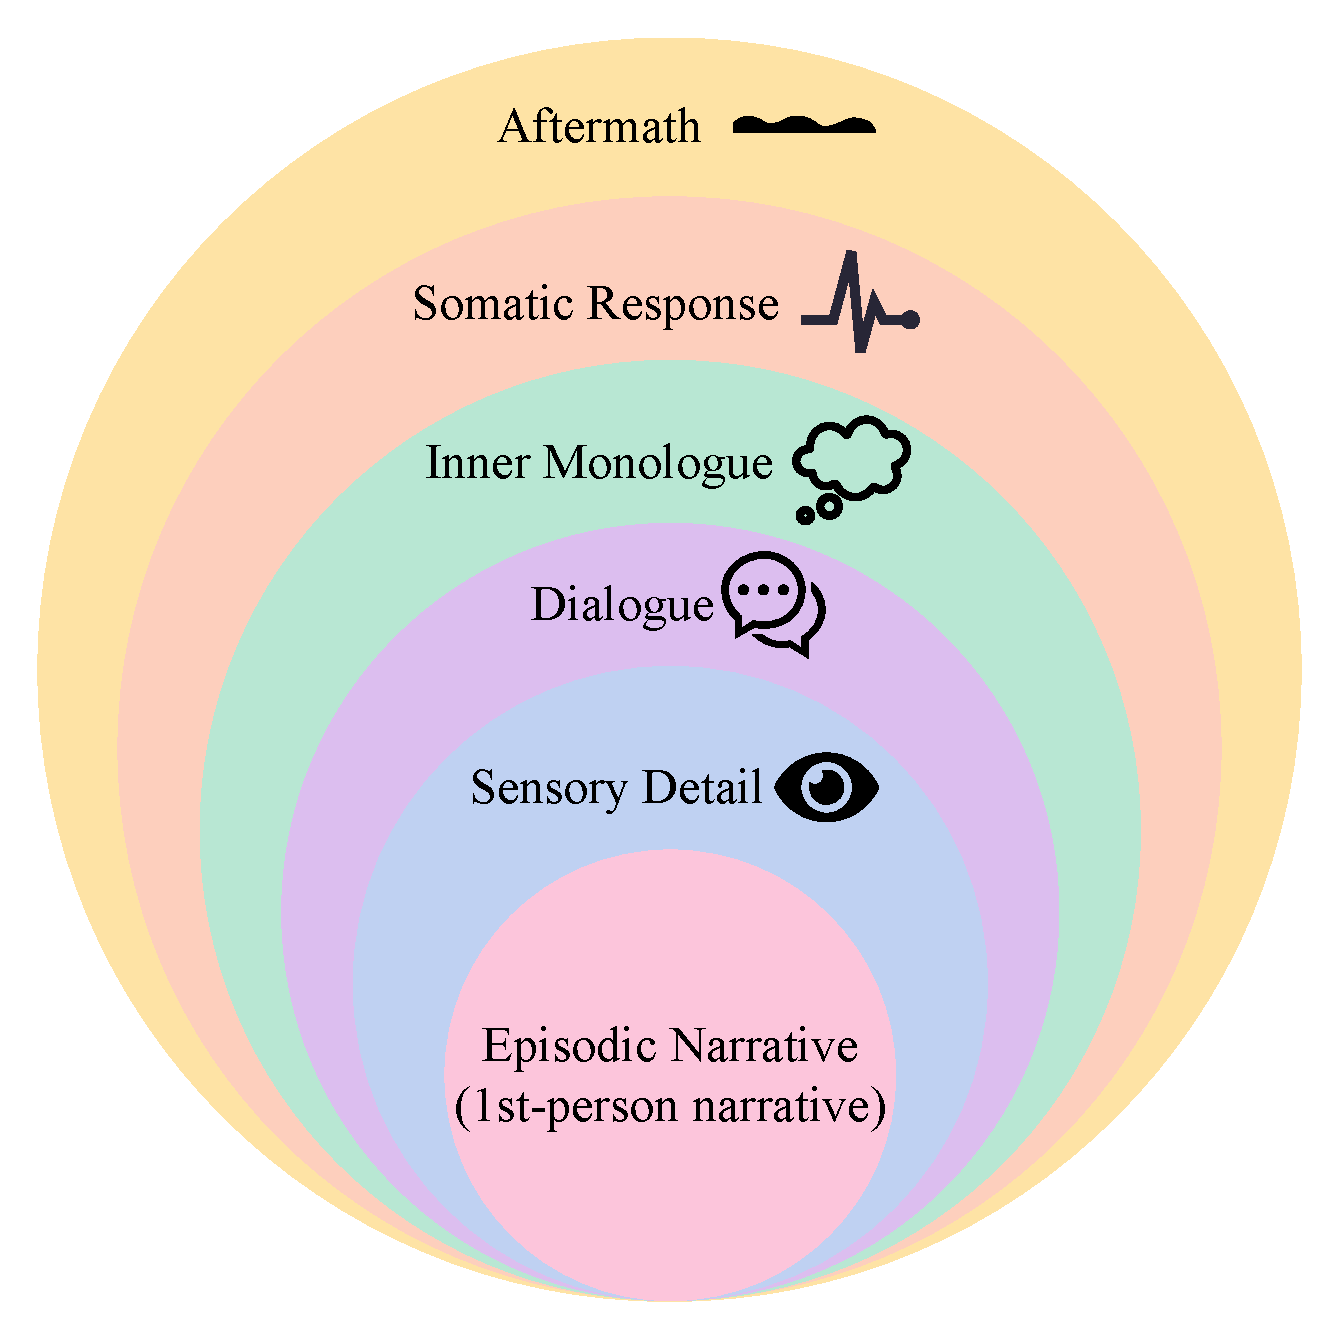
\includegraphics[width=0.8\linewidth]{figures/rubin_model.pdf}
\caption{Five operational dimensions, inspired by Rubin's Basic Systems Model~\cite{rubin2006basic}, used to structure synthetic episodic narratives.}
\label{fig:rubin}
\vspace{-10pt}
\end{figure}

\textbf{Stage 3: Quality Audit.} Each memory is screened against six automated defect criteria covering perspective drift, age-inappropriate retrospection, metadata leakage, duplication, length, and over-psychologization. Of the 11{,}000 memories, 8{,}991 passed the initial automated audit, 1{,}935 passed after automated rewriting, and 74 were escalated to the same four-expert team introduced above. The professor revised 71 memories, all of which subsequently passed the LLM judge; the other three were unanimously accepted by the reviewers as false-positive LLM flags. Accepted memories are then deduplicated, chronologically ordered into a 1,000-entry timeline, and sanitized with gender-neutral labels. Full criteria and repair procedures appear in Appendix~\ref{app:stage_d}, with the final schema and statistics in Appendix~\ref{app:stats}.

\subsection{Scenario Construction}
\label{sec:scenario}

%We construct a set of scenarios to evaluate whether LLMs can exhibit human-like, persona-consistent behavior under diverse contexts.
A scenario defines a character-agnostic decision context that serves as a shared external stimulus in our evaluation (see Appendix~\ref{app:ExampleofScenario} for a complete example). Each compatible character is placed in the same environmental and narrative context and required to respond to a decision-triggering event. During evaluation, every LLM receives the scenario, options, character ID, and occupation; memory-augmented settings additionally provide retrieved synthetic memories. The model must identify the response keyed to the target character. By holding the external situation fixed across characters, scenarios enable controlled comparison of whether LLMs can distinguish response differences encoded in the predefined profiles and synthetic histories.

% ---- Formal Notation ----
Formally, a scenario is represented as $s=\langle m,\mathcal{C}_{\mathrm{env}},\mathcal{C}_{\mathrm{narrative}},e_{\mathrm{trigger}}\rangle$, where $m$ contains the scenario metadata, including its target life-stage bin and intensity; $\mathcal{C}_{\mathrm{env}}$ and $\mathcal{C}_{\mathrm{narrative}}$ specify the environmental and narrative contexts, respectively; and $e_{\mathrm{trigger}}$ denotes the event that prompts an immediate response.

We construct the scenario suite through a three-stage human-in-the-loop pipeline: expert blueprinting, LLM-assisted expansion, and expert review.

\textbf{Stage 1: Human-Guided Blueprinting.} 
To ensure structural diversity, clinical experts manually draft the foundational summaries for all scenarios, using the DIAMONDS~\cite{rauthmann2014diamonds} framework to structure coverage of situational dimensions. We design exactly 8 scenarios per life-stage bin, yielding 64 scenarios across eight bins. These summaries cover family, school, workplace, relationship, and public-space contexts. Each summary establishes a core tension while maintaining the character-agnostic constraint.

\textbf{Stage 2: LLM-Assisted Expansion.}
We use Claude Opus 4.6~\cite{anthropic2026opus46} to expand the expert-drafted summaries into structured scenario descriptions based on a four-component schema (metadata, environmental setting, narrative context, and trigger event), enforcing consistent fields across age metadata and context. The full schema and a complete worked example are given in Appendix~\ref{app:scenario_schema}.

% For example, a human-designed summary for adolescence intellectual challenge becomes a detailed scenario titled "The Classroom Dissent," where a 15-year-old student discovers contradictions between their teacher's historical account and recent academic research they read independently. The scenario specifies the classroom setting ("quiet, dull, slightly oppressive atmosphere"), provides rich narrative context about the authority dynamics, and culminates in the teacher directly asking the student to share their thoughts, requiring a decision on whether to challenge authority with evidence-based disagreement (see Appendix~\ref{app:ExampleofScenario}).
\textbf{Stage 3: Expert Review.} Two doctoral-level psychology researchers review the generated scenarios for logical plausibility and assess their coverage using two theory-informed lenses: DIAMONDS~\cite{rauthmann2014diamonds} ratings describe the eight situational dimensions at varying intensity levels, and Schwartz's value circumplex~\cite{schwartz1992universals} is used to check intended value-conflict alignment. The resulting rating and conflict distributions document coverage under this designed scenario set (protocol and full distributions in Appendix~\ref{app:scenario_validation}).

\begin{figure*}[t]
\centering
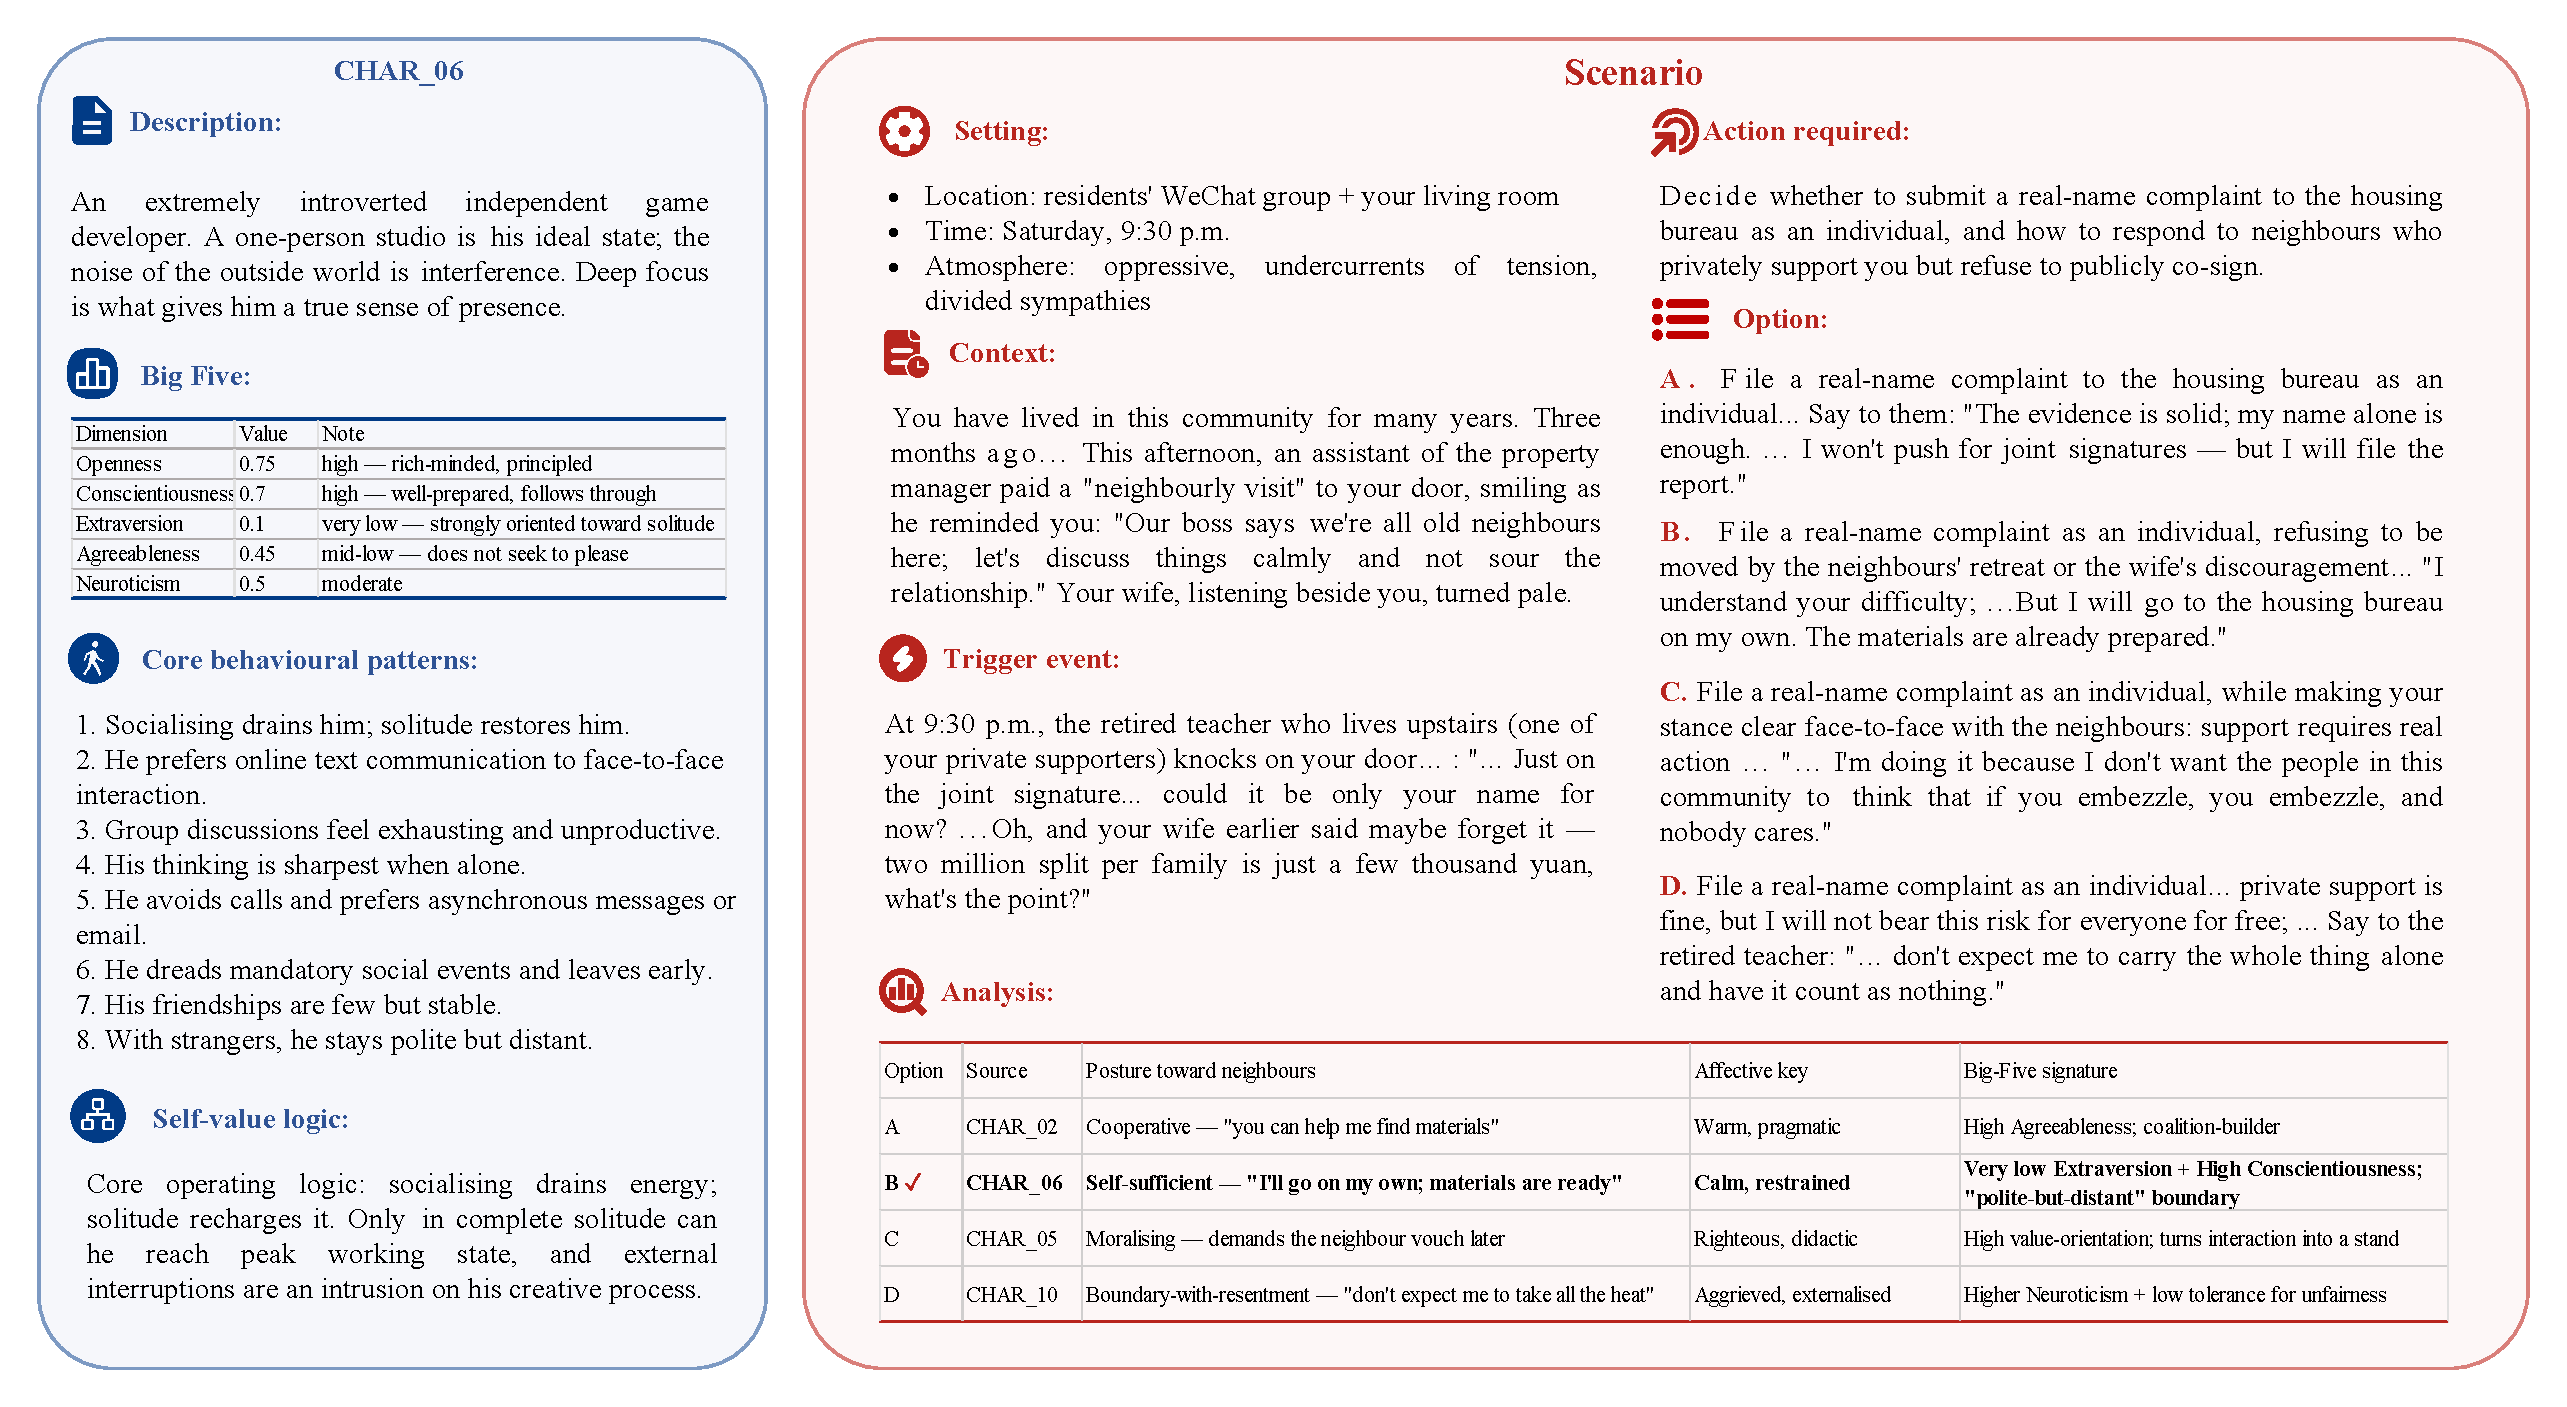
\includegraphics[width=1\linewidth]{figures/case_study.pdf}
\caption{A \ourbench instance requiring profile--response alignment beyond surface action matching; detailed analysis is in Appendix~\ref{app:case_study}.}
\label{fig:case_study}
\vspace{-10pt}
\end{figure*}

\subsection{Creating Evaluation Instances}
\label{sec:CreatingEvaluationInstances}

Having built the character and scenario sets, we formulate each test instance as an MCQ whose keyed reference is the response judged by experts to be most consistent with the predefined target character, its synthetic history, and the scenario. This adjudicated response serves as the benchmark label.

\Needspace{3\baselineskip}
\textbf{Stage 1: Automated Annotation with LLMs.}
For each (character, scenario) pair, the predefined profile (Big Five traits, Schwartz values, and self-narrative) serves as the primary character specification, while the scenario defines the decision context. Three parallel family-specific pipelines (Claude, GPT, and Gemini) each retrieve relevant episodic memories and use them alongside the profile and scenario to generate a candidate response. The memories provide experiential context, with their model-generated annotations serving as auxiliary cues for interpreting the situation and supporting behavioral judgments; different memory sets can provide plausible support for the same scenario. Using multiple model families reduces dependence on any single annotation model and provides diverse candidates for expert comparison. Candidate order is randomized and model-family identities remain hidden throughout review. Full model configurations, prompts, and an annotation example are provided in Appendix~\ref{app:annotation}.

\Needspace{3\baselineskip}
\textbf{Stage 2: Expert Review and Adjudication.}
The same four-expert team introduced in Section~\ref{sec:character} reviews and adjudicates the reference responses. The three researchers serve as primary annotators, independently assessing pair suitability and comparing anonymized candidates for persona consistency, situational fit, and grounding in their associated memories, while the senior professor serves as arbitrator. Under a consensus-then-arbitration rule, a candidate is adopted directly only when all three annotators select it as \textit{acceptable as-is}; otherwise, the arbitrator selects, edits, or rewrites the response, or discards an unsuitable pair. This process removed $31$ pairs and retained $673$ expert-adjudicated reference responses. Experts changed approximately $15\%$ of the words in selected LLM candidates on average, documenting substantive human involvement in constructing the references. Full guidelines and outcome statistics are provided in Appendix~\ref{app:annotation_protocol}.

\Needspace{3\baselineskip}
\textbf{Stage 3: Test Instance Assembly.}
For each retained annotation, the target character's adjudicated response becomes the keyed reference option, while \textit{Claude-Sonnet-4.6}~\cite{anthropic2026sonnet46} selects three distractors from the available adjudicated responses associated with other characters in the same scenario. The selection excludes responses that are either too similar to the reference or obviously irrelevant, avoiding ambiguous or trivial questions. The four options are randomly shuffled to remove positional bias, yielding $673$ MCQs. Full assembly rules are provided in Appendix~\ref{app:mcq_assembly}.

Claude-Sonnet-4.6 screened all $673$ assembled MCQs against six option-quality criteria, and all passed the screen (Appendix~\ref{app:mcq_screening}). Separately, three experts independent of the original construction team assessed a stratified random subset of 176 final MCQs. All three experts supported the existing reference option on 139 items (79.0\%), while two of three supported it on the remaining 37 items (21.0\%); thus, every sampled item received majority support for the existing key. Pre-adjudication inter-rater reliability was high (Fleiss' $\kappa=0.81$; Krippendorff's $\alpha=0.81$). All 37 items without complete agreement entered adjudication, and the adjudicator confirmed that each item and keyed answer was usable as-is. No wording edits or keyed-answer changes were required, and the audit did not alter the evaluated dataset or primary scores. These results support reference-label reliability on the audited subset. The full protocol and results are provided in Appendix~\ref{app:independent_calibration}.

\begin{table*}[t]
\centering
\caption{Accuracy on \ourbench. Memory-Aug. Avg. averages the three retrieval-based settings, excluding No-Retrieval. Gemini-3.1-Pro performs best. Scenario-clustered 95\% CIs are in Appendix~\ref{app:statistical_analysis}.}
\vspace{-5pt}
\label{tab:main_results}
\setlength{\tabcolsep}{6pt}
\small
\resizebox{\textwidth}{!}{%
\begin{tabular}{lc|ccc|c}
\toprule
\textbf{Model} & \textbf{No-Retrieval LLM} & \textbf{Naive-RAG} & \textbf{Mem0} & \textbf{PersonaDB} & \textbf{Memory-Aug. Avg.} \\
\midrule
\noalign{\vskip -2pt}
\multicolumn{6}{l}{\textit{Open-source}}\\[-2pt]
\midrule
\quad DeepSeek-V3.2              & 0.285 & 0.412 & 0.425 & 0.428 & 0.422 \\
\quad DeepSeek-V4-Flash          & 0.278 & 0.348 & 0.336 & 0.328 & 0.337 \\
\quad DeepSeek-V4-Pro            & 0.291 & 0.407 & 0.372 & 0.367 & 0.382 \\
\quad Qwen3.5-35B-A3B            & 0.254 & 0.370 & 0.372 & 0.366 & 0.369 \\
\quad Qwen3.5-122B-A10B          & 0.264 & 0.391 & 0.394 & 0.389 & 0.391 \\
\quad Qwen3.5-397B-A17B          & 0.275 & 0.403 & 0.406 & 0.404 & 0.404 \\
\midrule
\noalign{\vskip -2pt}
\multicolumn{6}{l}{\textit{Closed-source}}\\[-2pt]
\midrule
\quad GPT-5.4-mini               & 0.288 & 0.330 & 0.343 & 0.322 & 0.332 \\
\quad GPT-5.4                    & 0.278 & 0.372 & 0.366 & 0.351 & 0.363 \\
\quad Claude-Haiku-4.5           & 0.245 & 0.357 & 0.363 & 0.376 & 0.365 \\
\quad Claude-Sonnet-4.6          & 0.257 & 0.401 & 0.389 & 0.401 & 0.397 \\
\quad Gemini-3-Flash             & 0.253 & 0.563 & 0.541 & 0.525 & 0.543 \\
\quad Gemini-3.1-Pro             & 0.264 & \textbf{0.633} & \textbf{0.624} & \textbf{0.624} & \textbf{0.627} \\
\bottomrule
\end{tabular}
}
\vspace{-10pt}
\end{table*}

\subsection{Example of \ourbench}
Figure~\ref{fig:case_study} illustrates profile--response alignment beyond surface action matching. CHAR\_06 combines very low Extraversion (0.10), high Conscientiousness (0.70), and a ``polite-but-distant'' interaction pattern. Option A preserves the complaint action but adds coalition building, whereas Options C and D introduce moralizing and blame. Experts keyed Option B because its prior preparation, individual action, and concise low-contact wording best match the encoded profile. The example shows how shared actions can differ in persona-specific pragmatic framing; Appendix~\ref{app:case_study} provides a fuller analysis.

\label{gen_inst}

\section{Experiments}

\subsection{Experimental Setup}

\paragraph{Model Selection.}
We evaluate 12 representative LLMs, including six open-source models: \textit{DeepSeek-V3.2}~\cite{deepseek_v3_2_2025}, \textit{DeepSeek-V4-Flash}, \textit{DeepSeek-V4-Pro}~\cite{deepseek_v4_2026}, \textit{Qwen3.5-35B-A3B}, \textit{Qwen3.5-122B-A10B}, and \textit{Qwen3.5-397B-A17B}~\cite{qwen35_2026}; and six closed-source models: \textit{GPT-5.4-mini}, \textit{GPT-5.4}~\cite{openai2026gpt54}, \textit{Claude-Haiku-4.5}~\cite{anthropic2025haiku45}, \textit{Claude-Sonnet-4.6}~\cite{anthropic2026sonnet46}, \textit{Gemini-3-Flash}~\cite{google2025gemini3flash}, and \textit{Gemini-3.1-Pro}~\cite{google2026gemini31pro}. All models are evaluated under a unified, deterministic decoding protocol (Appendix~\ref{app:decoding}).

\paragraph{Memory-Augmented Settings.}
We compare three retrieval-based frameworks---Naive-RAG~\cite{lewis2020retrieval}, Mem0~\cite{chhikara2025mem0}, and PersonaDB~\cite{sun2025persona}---against a \textit{No-Retrieval LLM} baseline. During evaluation, all models receive the scenario, answer options, character ID, and occupation. For all three memory-augmented settings, both the memory backend and the model-facing prompt use only the de-identified \texttt{content\_full} narrative; no other stored memory field enters the evaluation pipeline. All retrieval frameworks use the same embedding and auxiliary memory-management models, with retrieval budgets calibrated to provide comparable episodic content. The underlying Big~Five vector, value logic, behavioral patterns, and structured psychological annotations are withheld to prevent direct reference-label leakage. Full implementation and field-isolation details are provided in Appendix~\ref{app:interactive_settings}; the model-facing evaluation template is reproduced in Appendix~\ref{app:prompt_evaluation}.

\paragraph{Evaluation Metrics.} We report \textit{accuracy}, defined as the proportion of the 673 MCQs for which a model selects the expert-adjudicated keyed option. Only the model's \texttt{decision\_choice} field is scored; the accompanying free-text rationale fields are not compared with the reference response and do not enter the metric. This metric quantifies agreement with \ourbench references. Statistical procedures are detailed in Appendix~\ref{app:statistical_analysis}.
Reference construction uses richer profile information than evaluation. Accuracy therefore jointly reflects retrieval coverage, recovery of persona cues, and agreement with expert-adjudicated references; it should not be interpreted as decision quality given an explicit profile (Appendix~\ref{app:interactive_settings}).
%$$\text{Accuracy} = \frac{\#\text{correct MCQs}}{\#\text{total MCQs}}.$$

\subsection{Results and Discussion}

\paragraph{Model choice dominates within the benchmark.} Under Naive-RAG, the spread between the best- and worst-performing models exceeds 30\% (63.3\% vs.\ 33.0\%), whereas the average gap between retrieval methods for a given model is only 1.7\% and never exceeds 4\%. The model- and method-axis Gini mean differences are 0.088 and 0.006, respectively, yielding a difference of 0.082 (95\% CI 0.068--0.096). Gemini-3.1-Pro achieves the best accuracy (63.3\%, 95\% CI 59.2--67.4\%) and ranks first by Memory-Augmented Avg. in all 10{,}000 scenario-bootstrap resamples. All non-Gemini models achieve only 33.2\%--42.2\% Memory-Augmented Avg., showing limited agreement with the expert-adjudicated references for synthetic characters under this setup.

\begin{table}[t]
\centering
\caption{Memory-content ablation on the 176-item subset. Accuracy is averaged over the 12 LLMs.}
\vspace{-5pt}
\label{tab:memory_ablation_summary}
\setlength{\tabcolsep}{2pt}
\small
\resizebox{\linewidth}{!}{%
\begin{tabular}{cllr}
\toprule
\textbf{Cond.} & \textbf{Character source} & \textbf{Memory selection} & \textbf{Acc.} \\
\midrule
C0 & Target & Target scenario & \textbf{0.399} \\
C1 & Target & Other same-bin scenario & 0.347 \\
C2 & Other & Target scenario & 0.227 \\
C3 & Target & Random non-target & 0.343 \\
\bottomrule
\end{tabular}
}
\vspace{-10pt}
\end{table}

\paragraph{Retrieval helps, with no significant differences among backends.} Retrieval outperforms No-Retrieval in all 36 Holm-corrected tests, whereas no comparison among the three retrieval backends is significant. Rankings remain strongly correlated across backends ($\rho=0.89\text{--}0.94$), and Mem0 and PersonaDB have lower point estimates than Naive-RAG for 6 and 8 of the 12 models, respectively. Their additional summarization and structural abstraction may obscure latent character cues in the original episodic memories, although the nonsignificant backend comparisons do not establish equivalence.

\paragraph{Memory ownership and scenario alignment are both informative.} On a fixed 176-item subset, we evaluate the same 12 models under Naive-RAG with $k{=}30$ while varying only the supplied memory assignment: C0 uses target-scenario memories from the target character; C1 uses memories retrieved for another scenario in the same life-stage bin from the target character; C2 uses target-scenario memories from another character; and C3 uses randomly sampled eligible non-target memories from the target character. The scenario, answer options, model, decoding protocol, and number of supplied memories are held fixed; no condition exposes the latent Big~Five vector, Schwartz profile, self-value logic, or behavioral templates. C0 achieves 39.9\% accuracy, exceeding C1, C2, and C3 by 5.23, 17.24, and 5.65 percentage points, respectively, with all 12 models favoring C0 in each contrast. Across paired model units, all three C0 contrasts remain significant under two-sided exact sign-flip tests after Holm correction over six comparisons (adjusted $p{=}0.00293$ for each). Thus, scenario-matched, character-owned memories provide information beyond either arbitrary same-character memories or scenario-matched memories from another character. Full protocol and per-model results are provided in Appendix~\ref{app:memory_ablation}.

% \begin{figure}[t]
% \centering
% \includegraphics[width=0.7\linewidth, trim=0 0 0 0 clip]{figures/radar_3configs_v2.png}
% \caption{Radar chart of behavioral accuracy for all 12 models under three retrieval configurations. Each spoke represents a model; models are grouped by family (color-coded arcs). The three polygons---Naive-RAG (solid), Mem0 (dashed), PersonaDB (dotted)---overlap closely for every model, confirming that the retrieval paradigm has little effect on rank order.}
% \label{fig:radar_configs}
% \end{figure}
% \begin{figure}[h]
% \centering
% \begin{minipage}{0.49\textwidth}
%     \centering
%     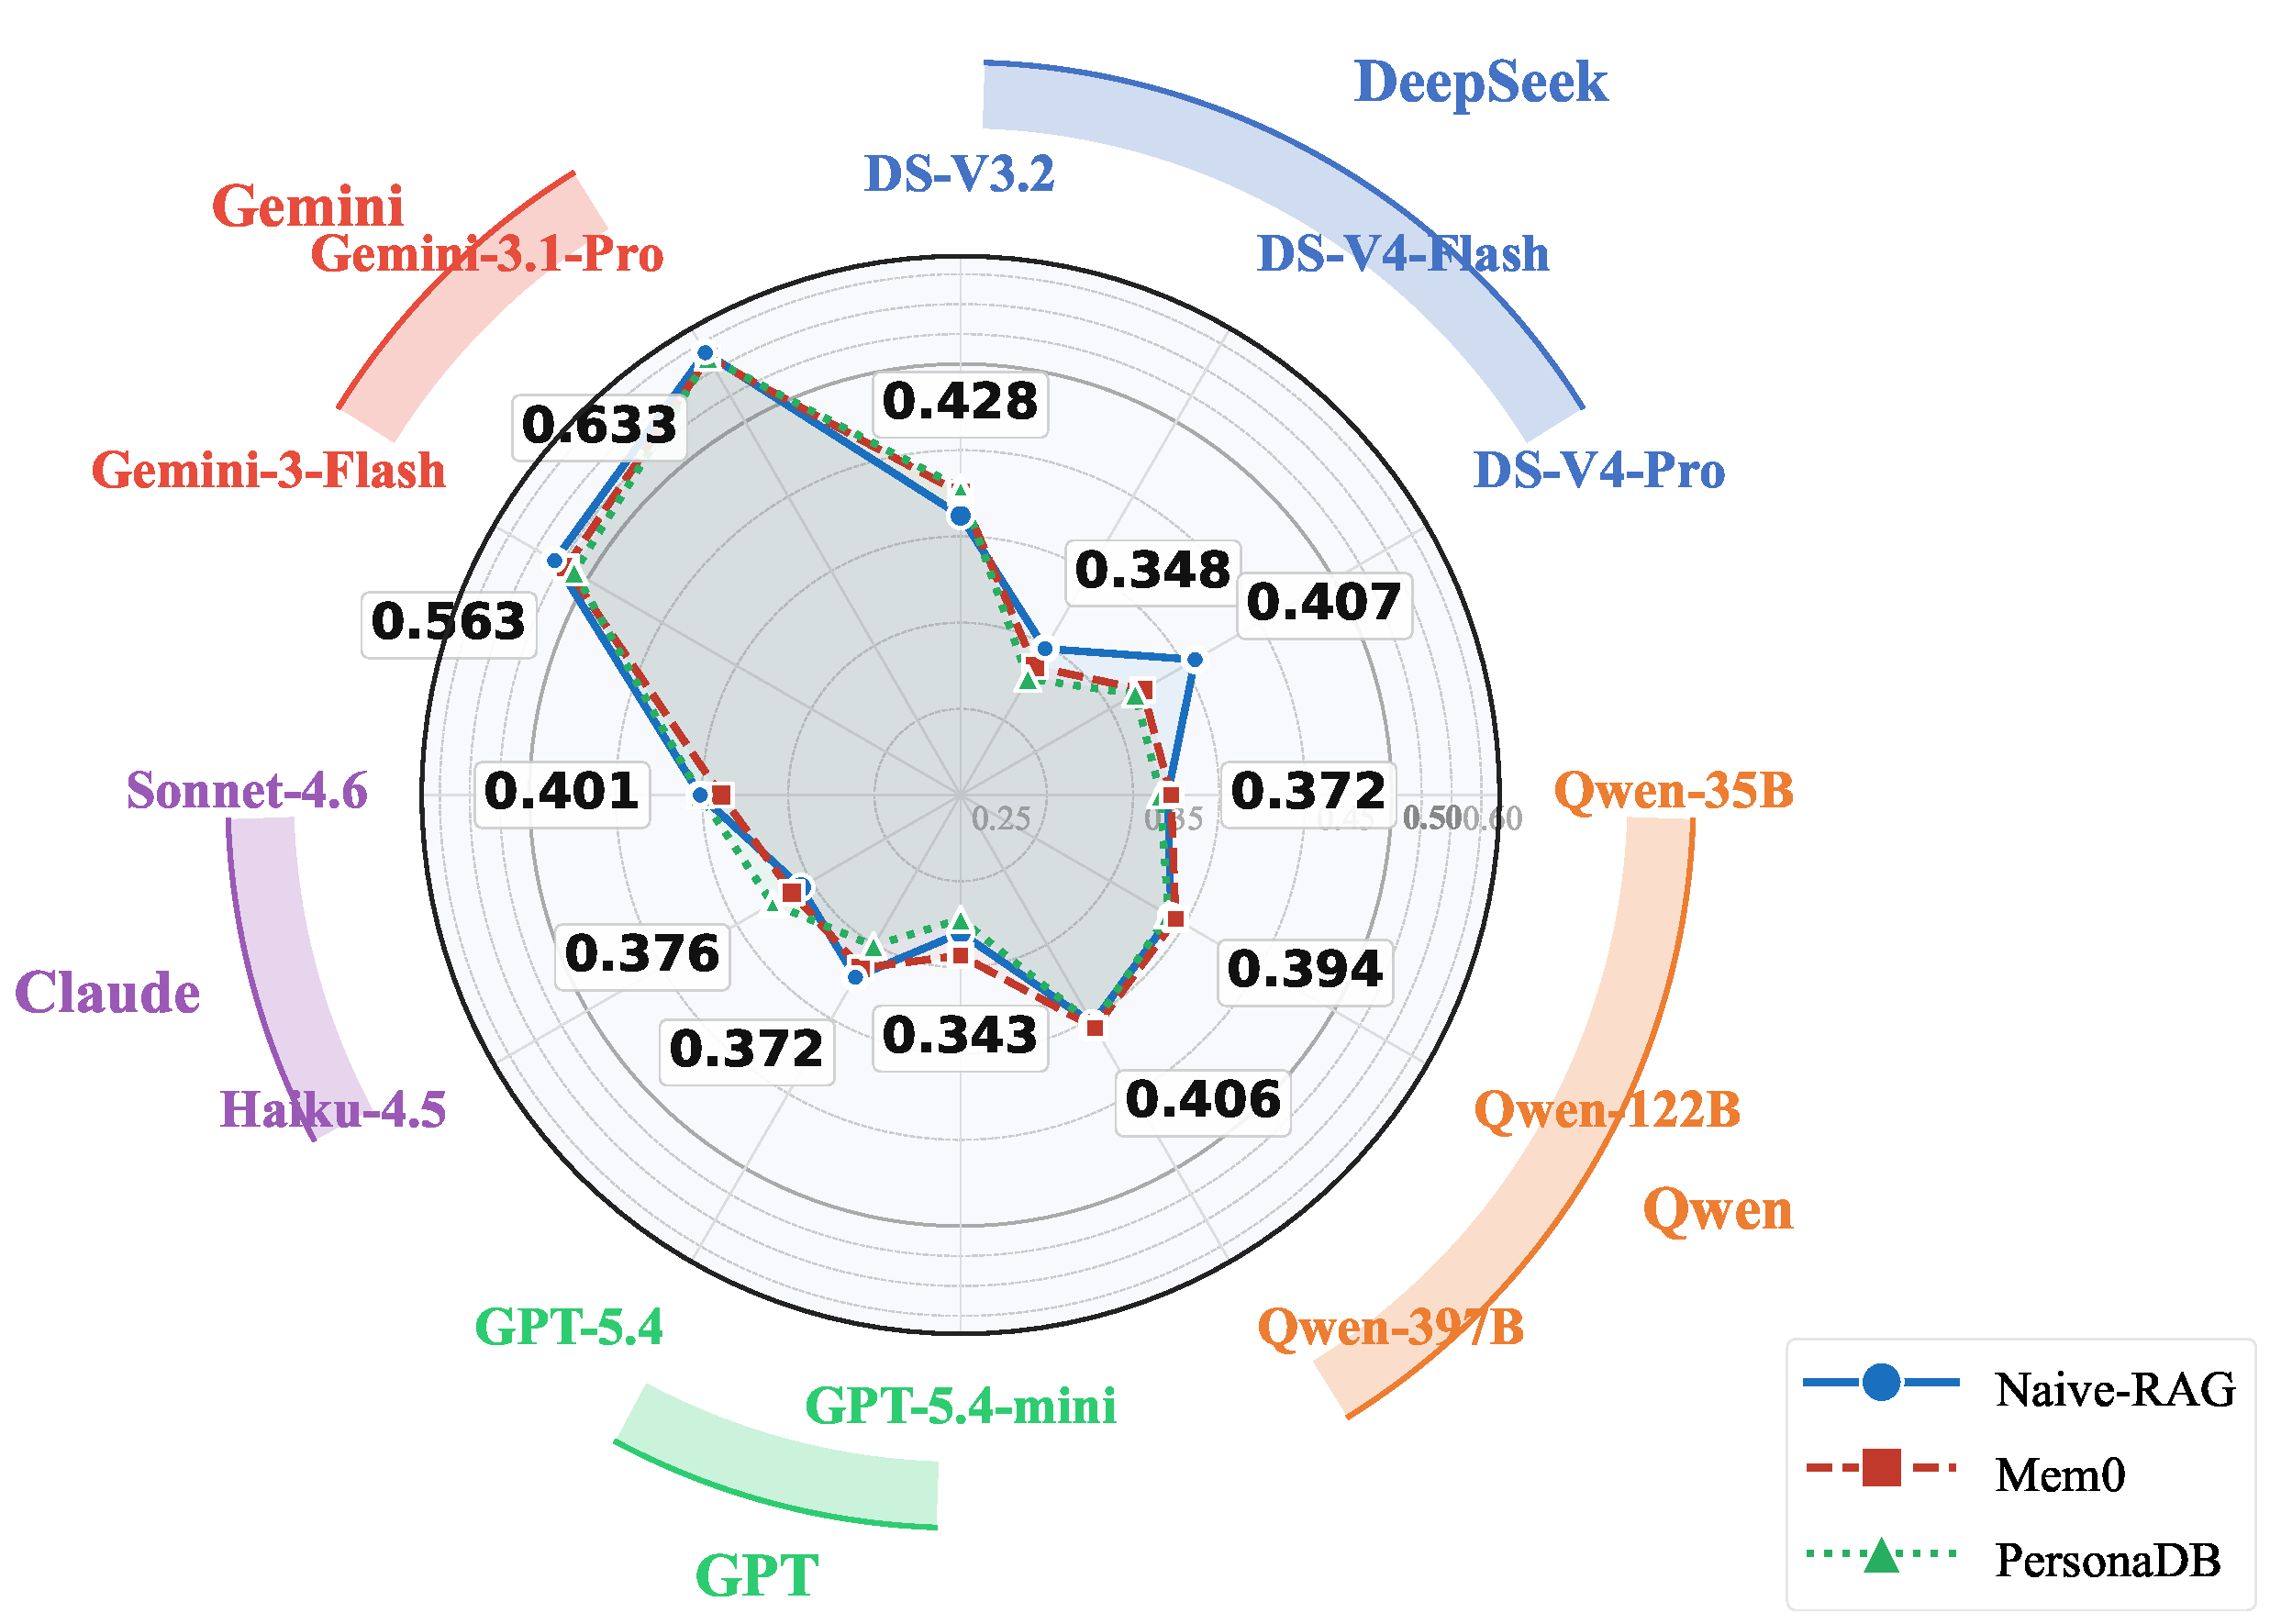
\includegraphics[width=\linewidth]{figures/radar_3configs_v2.pdf}
%     \caption{Behavioral accuracy for all 12 models, shown separately for the three interactive settings. Each spoke represents a model; models are grouped by family (color-coded arcs). 
%     % The three polygons overlap closely across all models, confirming that the retrieval paradigm has little effect on the rank order.
%     } 
%     \label{fig:radar_configs}
% \end{minipage}
% \hfill
% \begin{minipage}{0.49\textwidth}
%     \centering
%     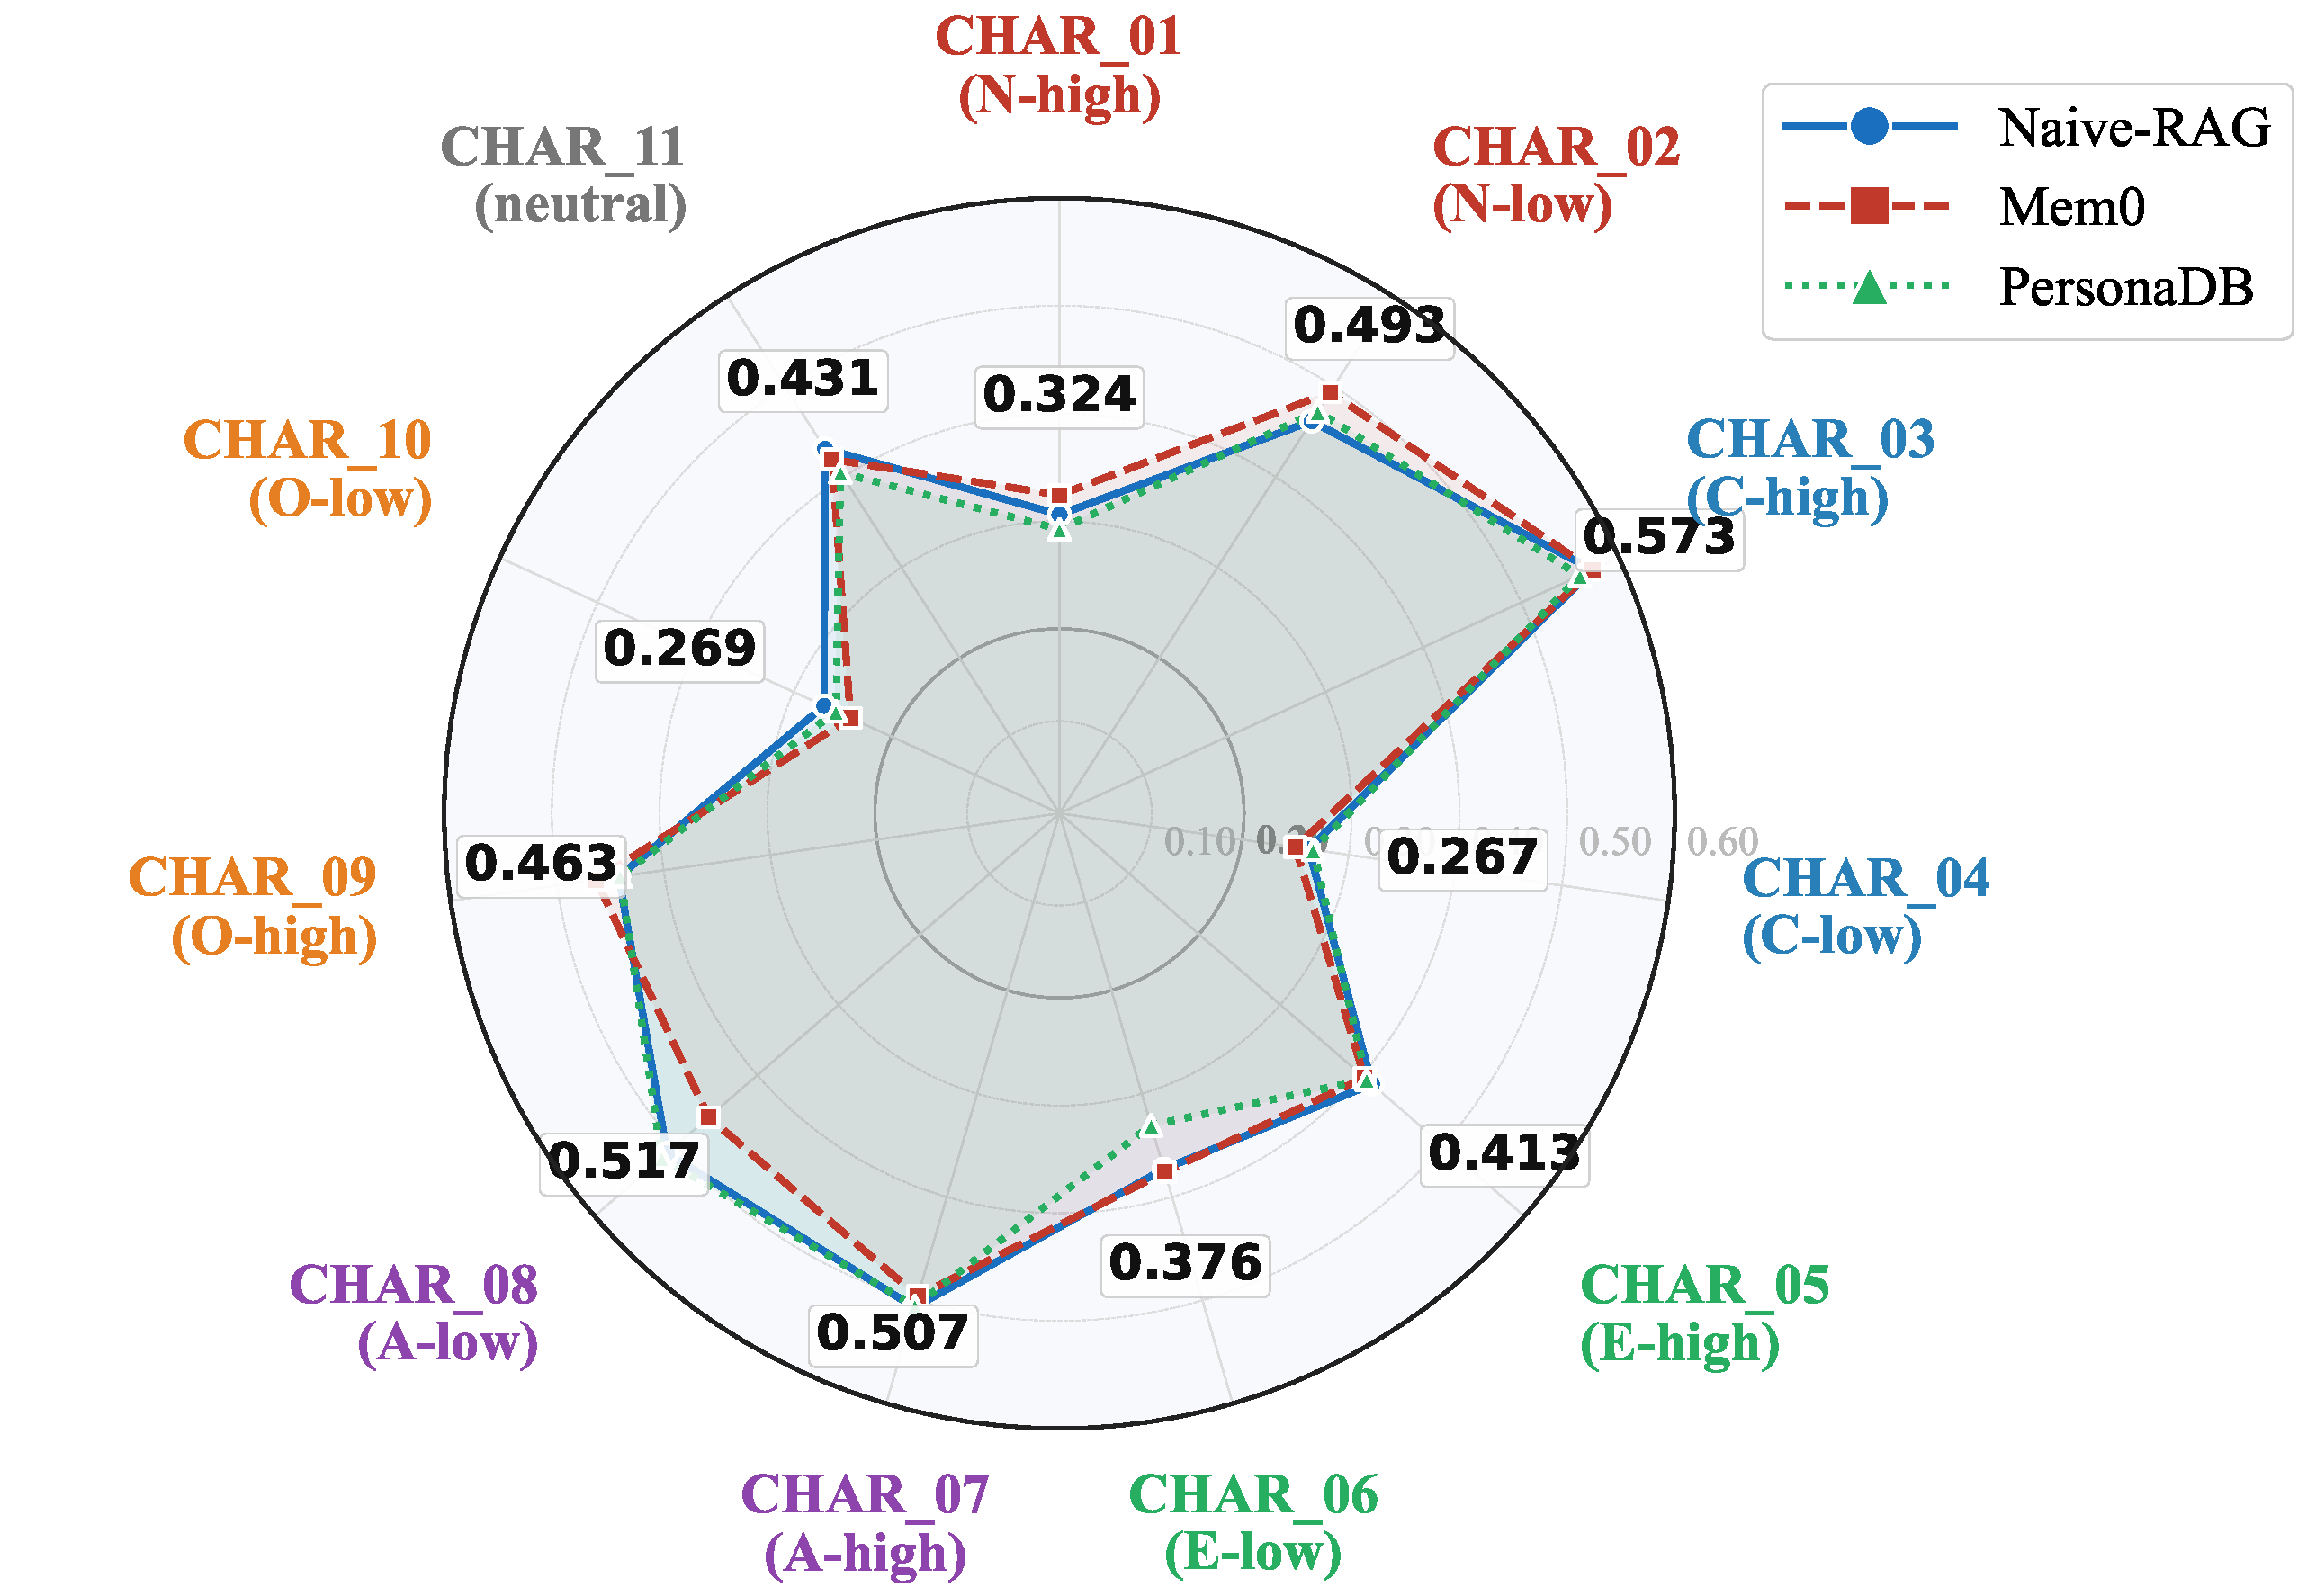
\includegraphics[width=\linewidth]{figures/fig_per_character_radar.pdf}
%     \caption{
%     Per-character behavioral accuracy averaged over evaluated LLMs for each interactive setting. Characters sharing a Big Five dimension use the same color.
%     % Per-character behavioral accuracy for the best model (Gemini-3.1-Pro, Naive-RAG). Characters defined by the same Big Five dimension are annotated with the same color. 
%     % High-N and high-C characters consistently yield higher accuracy, suggesting that extreme personality signatures leave stronger traces in autobiographical memory that current models can exploit.
%     }
%     \label{fig:per_char_radar}
% \end{minipage}
% \vspace{-15pt}
% \end{figure}

\paragraph{Gemini's lead persists across reference-response provenance subsets.} Because Gemini-origin candidates account for 497 of the 673 adjudicated references, same-family annotation bias is a natural concern. Gemini-3.1-Pro and Gemini-3-Flash nevertheless remain the top two models by Memory-Augmented Avg. on the Gemini-origin (63.3\% and 54.2\%), Claude-origin (61.6\% and 56.1\%), and GPT-origin subsets (59.3\% and 50.0\%), with source-specific ranking correlations of $\rho=0.666$--$0.809$. On non-Gemini-origin items, the Gemini family retains a 17.3-point advantage. Provenance interactions are nonsignificant in both scenario-clustered difference-in-differences (4.9 points, 95\% CI $-1.1$--$10.8$, adjusted $p{=}0.3395$) and item-fixed-effect analyses (5.4 points, 95\% CI $-0.6$--$11.5$, adjusted $p{=}0.2759$). These analyses do not detect a statistically significant family-specific provenance interaction, although they do not establish the absence of source bias (Appendix~\ref{app:gt_source_results}).

\begin{figure}[t]
\centering
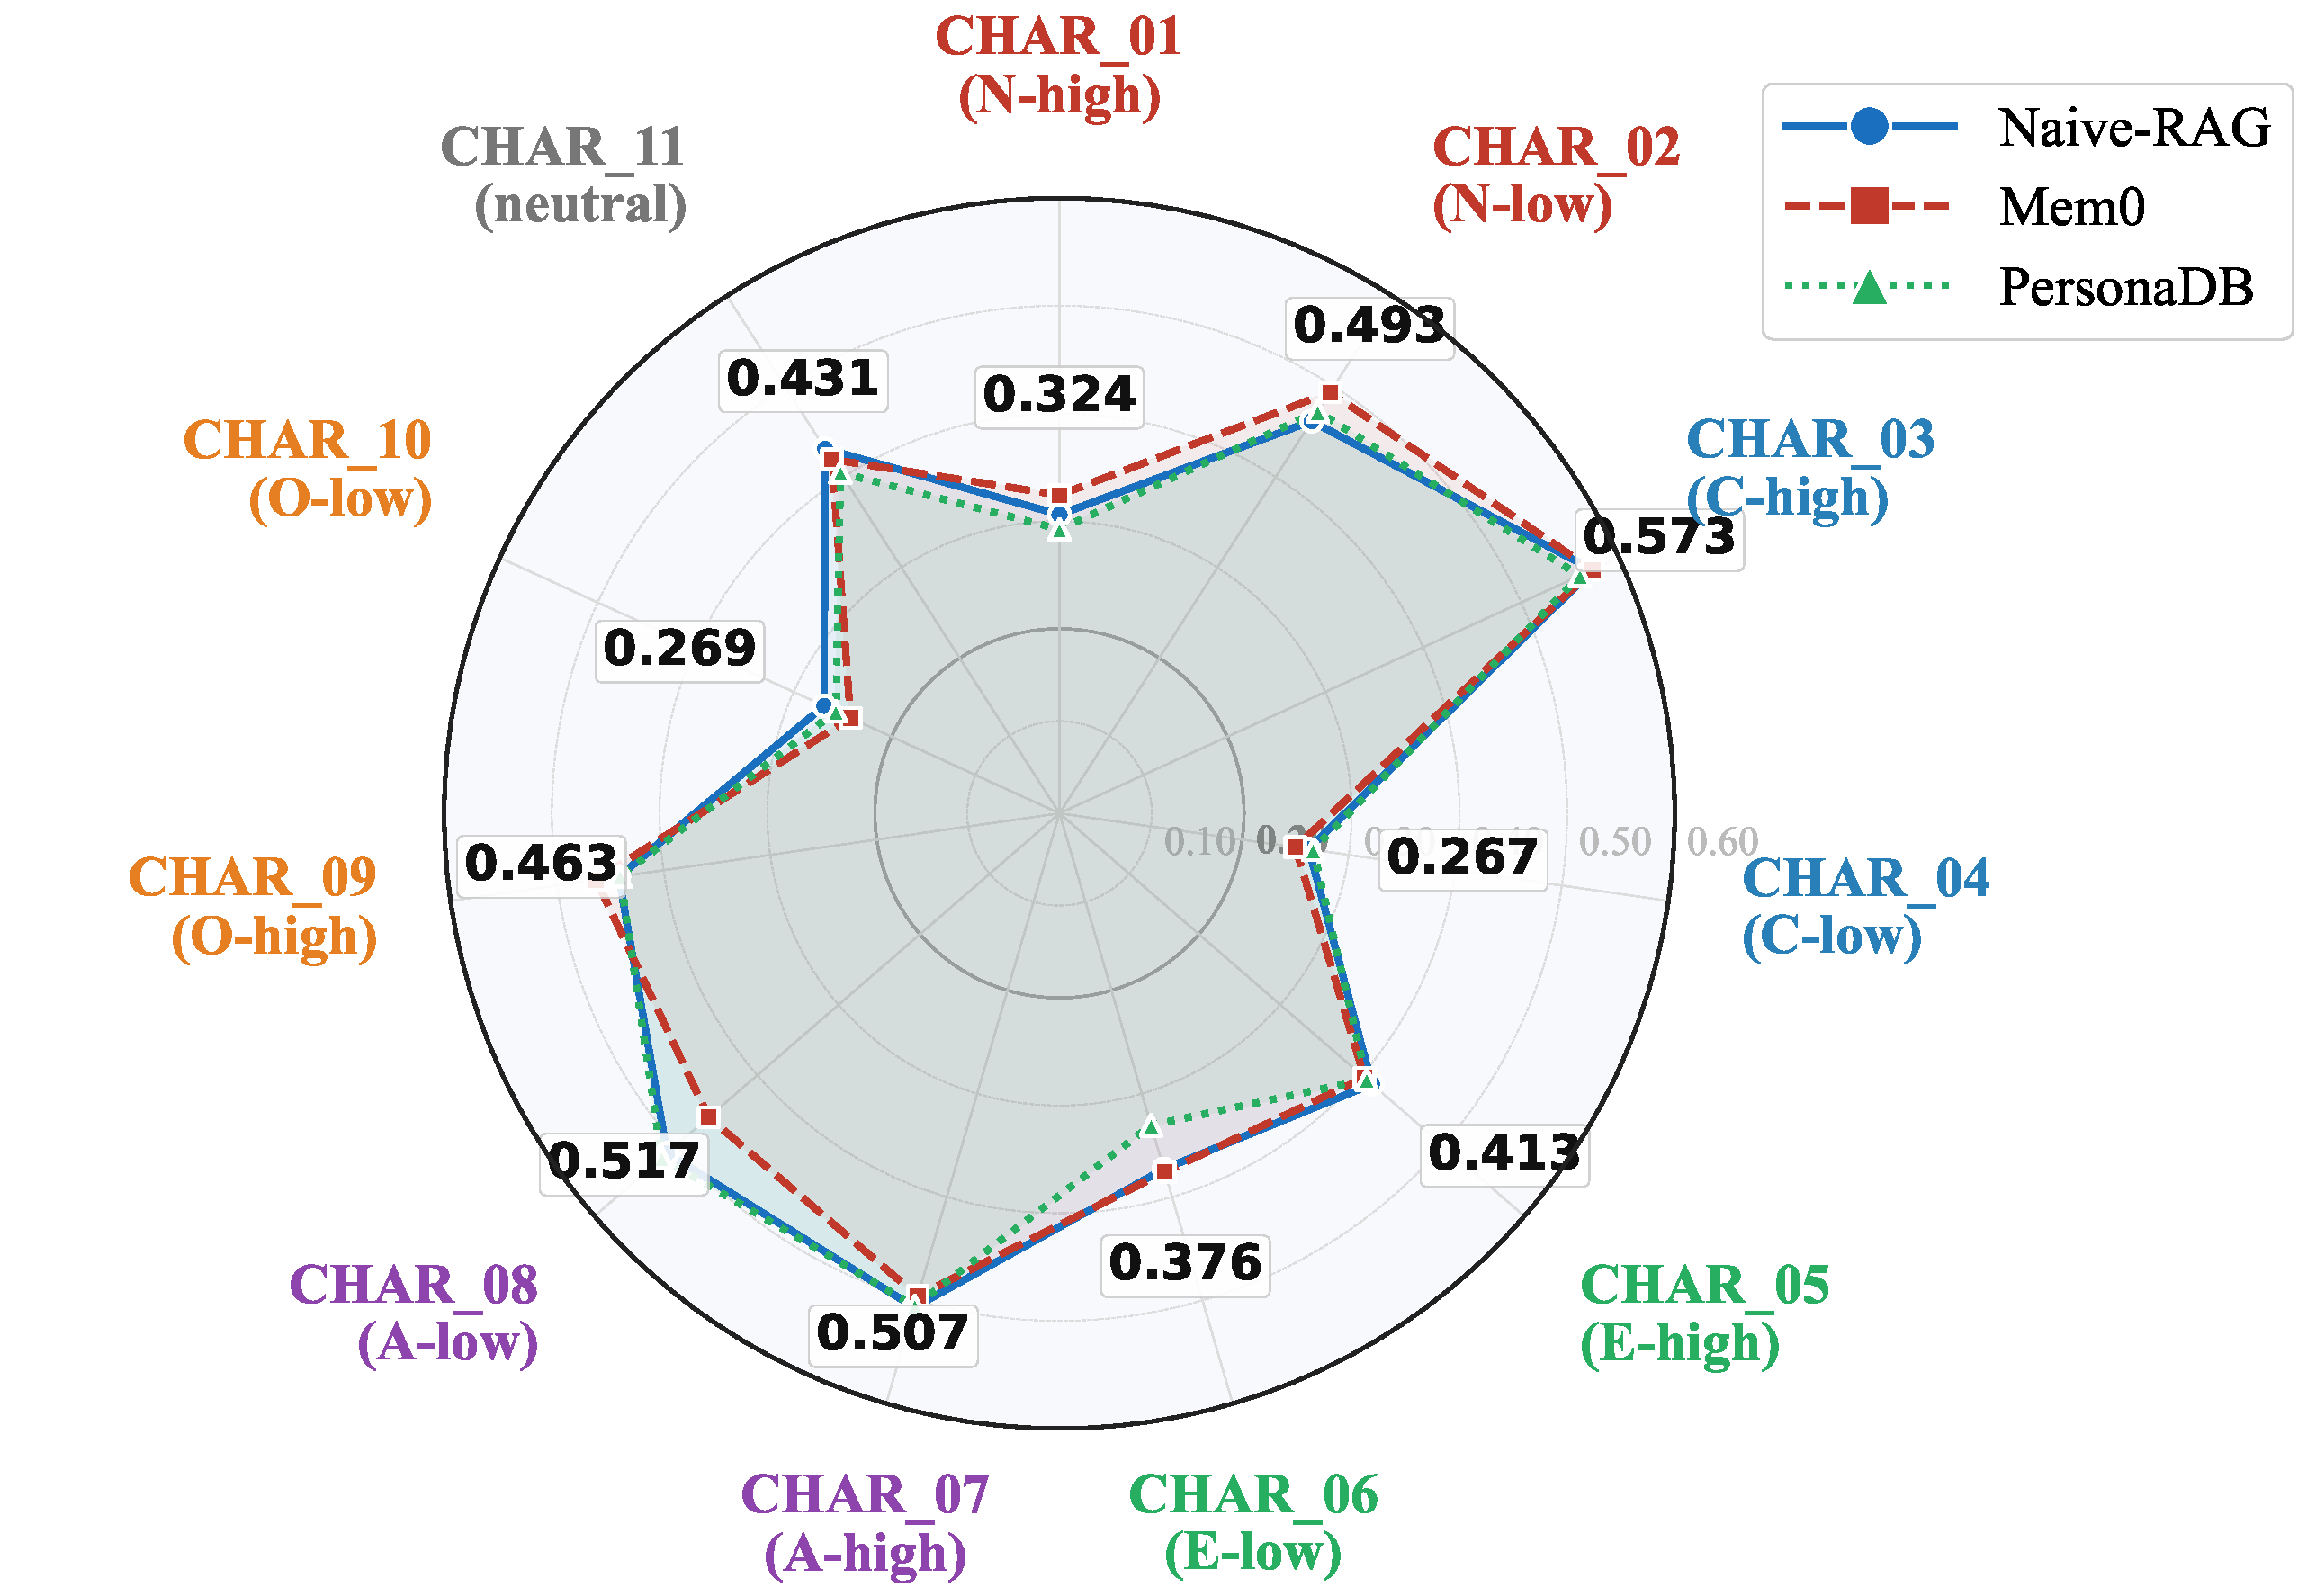
\includegraphics[width=\linewidth]{figures/fig_per_character_radar.pdf}
\caption{Per-character accuracy averaged across LLMs by memory-augmented setting.}
\label{fig:per_char_radar}
\vspace{-10pt}
\end{figure}

\paragraph{Character-level difficulty and error patterns.} Figure~\ref{fig:per_char_radar} shows substantial variation across characters: C-High (CHAR\_03) reaches 57.3\%, whereas C-Low (CHAR\_04, 26.7\%) and O-Low (CHAR\_10, 26.9\%) are the two hardest characters. N-High (CHAR\_01, 32.4\%) is also among the more difficult characters. Errors are concentrated: among 221 persistent shared-failure items, 84.2\% have at least half of the Naive-RAG models converging on the same non-reference option. Dominant confusions include C-Low$\to$C-High, N-High$\to$N-Low, and O-Low$\to$O-High, indicating structured opposite-pole errors rather than a uniform distribution.

\FloatBarrier
\section{Related Work}

\subsection{Persona Modeling in LLM Systems}
The Big Five (OCEAN) framework~\cite{mccrae1992introduction} is a prominent account of stable individual differences, with predictive validity across cultures~\cite{mccrae1997personality} and the lifespan~\cite{roberts2007power}. Human-personality research also describes behavioral states that vary with situational demands~\cite{fleeson2001toward}, autobiographical experiences organized around self-relevant goals~\cite{conway2000construction}, and developmental schemas associated with later reactions~\cite{young2006schema}. These theories motivate the structured synthetic artifacts in our benchmark.

Current LLM persona systems follow two broad lines. The first injects static role descriptions or trait vectors at inference time, as in Character-LLM~\cite{shao2023character}, PersonaLLM~\cite{jiang2024personallm}, PersonaAgent~\cite{zhang2025personaagent}, and RGMem~\cite{tian2025rgmem}. The second develops long-term memory infrastructure, including MemGPT~\cite{packer2023memgpt}, HippoRAG~\cite{gutierrez2024hipporag}, Mem0~\cite{chhikara2025mem0}, and A-MEM~\cite{xu2025mem}. Existing systems usually provide either static profiles or long-term memory stores; few benchmarks test response selection conditioned jointly on a predefined trait/value profile and its synthetic memory history.

\subsection{Benchmarks for Persona- and Psychology-Informed Evaluation}

\textbf{Psychometric evaluation of LLMs.}
Prompted LLMs can simulate Big Five questionnaire responses with reasonable reliability~\cite{serapio2023personality}, and related work uses MBTI or Big Five scales to characterize model behavior. However, these approaches treat psychometric instruments as stimuli rather than testing persona-consistent decisions in controlled scenarios. They also evaluate context-free snapshots rather than response selection conditioned jointly on a profile and a structured synthetic history~\cite{mcadams2001psychology,pasupathi2007developing}.

\paragraph{Persona and memory benchmarks.}
Conversational persona benchmarks generally test factual or stylistic consistency. Long-horizon benchmarks such as LoCoMo~\cite{maharana2024evaluating} and LongMemEval~\cite{wu2024longmemeval} extend evaluation to multi-session dialogue but primarily assess recall. CloneMem~\cite{hu2026clonemem}, RealMem~\cite{bian2026realmem}, and KnowMeBench~\cite{wu2026knowme} use richer personal evidence, yet their central targets remain recall, preference inference, or goal consistency. In contrast, \ourbench evaluates memory-grounded persona-consistent response selection under controlled scenarios structured by DIAMONDS~\cite{rauthmann2014diamonds}.

\paragraph{Data substrates and evaluation depth.}
Synthetic chat logs and task-oriented interactions often lack the perceptual, affective, and introspective detail represented in autobiographical memories~\cite{rubin2006basic}, making memory-grounded character reasoning difficult to distinguish from surface pattern matching. Existing benchmarks also rarely combine content-rich episodic narratives with explicitly age-indexed synthetic histories~\cite{mcadams2001psychology}. \ourbench addresses this gap by using dimensions inspired by Rubin's Basic Systems Model~\cite{rubin2006basic} to structure generated memories and organizing them into eight age-defined life-stage bins informed by developmental theories~\cite{erikson1963childhood,levinson1978seasons}.

\section{Conclusion}
In this work, we presented \ourbench, a controlled benchmark for memory-grounded, persona-consistent response selection in LLMs. It combines 11 predefined synthetic characters, 11{,}000 synthetic autobiographical memories, 64 shared decision scenarios, and 673 MCQs keyed by expert-adjudicated reference responses. Across 12 models and four evaluation settings, agreement with these references remains limited; the memory-content ablation further shows higher accuracy when supplied memories match both the target character and the scenario. The shared-scenario structure supports controlled comparisons of retrieval, memory representation, and persona-conditioned response selection methods. We intend \ourbench as a testbed for persona consistency and memory grounding.

\section*{Limitations}
\label{sec:limitations}
The central limitation is construct scope: \ourbench evaluates agreement with expert-adjudicated references for synthetic characters rather than behavior observed from real people. Expert review supports content plausibility and reference-label reliability. A single keyed option compresses potentially plural, context-dependent behavior, and the static MCQ format does not measure interactive agent behavior. Because several evaluated model families also contributed candidate responses, source-family or stylistic cues may remain despite anonymized expert adjudication and our provenance-stratified analysis.

The benchmark is also limited to 11 characters, 64 scenarios, and single-turn choices, restricting coverage of cultures, demographics, naturalistic interaction, and within-person change. Its expert-intensive construction limits scale, and the independent audit covers 176 of 673 items, supporting a dataset-level reliability estimate rather than item-wise validation of the full benchmark. Future work should incorporate human-authored candidates, distributions over plausible responses, multi-turn settings, and references derived from observed behavior to evaluate external validity.

% \clearpage
\bibliography{ref}

% ============================================================
%  Appendix for \ourbench
%  \input{} this file after \appendix in main.tex
%  Requires: booktabs, tabularx, enumitem packages
% ============================================================

% ---- Appendix Table of Contents ----
% \clearpage
% \begin{center}
%   {\LARGE\bfseries Appendices}
% \end{center}
% \vspace{2em}

% \newcommand{\appdots}{\hspace{0.3em}\leaders\hbox{\normalfont.}\hfill\hspace{0.3em}}

% \setlength{\parindent}{0pt}
% {\setlength{\parskip}{7pt}
% \textbf{\large A}\quad{\large\bfseries Benchmark Comparison Dimensions\appdots\pageref{app:benchmark_dims}}

% \textbf{\large B}\quad{\large\bfseries Character Construction and Memory Pipeline\appdots\pageref{app:character}}

% \hspace{2em}B.1\enspace Profile Specification\appdots\pageref{app:stage_a}

% \hspace{2em}B.2\enspace Memory Quota Allocation\appdots\pageref{app:stage_b}

% \hspace{2em}B.3\enspace Memory Generation Protocol\appdots\pageref{app:stage_c}

% \hspace{2em}B.4\enspace Quality Audit and Repair\appdots\pageref{app:stage_d}

% \hspace{2em}B.5\enspace Memory Schema\appdots\pageref{app:schema}

% \hspace{2em}B.6\enspace Dataset Statistics\appdots\pageref{app:stats}

% \textbf{\large C}\quad{\large\bfseries Scenario Construction and Validation\appdots\pageref{app:scenario}}

% \hspace{2em}C.1\enspace Scenario Schema and Example\appdots\pageref{app:scenario_schema}

% \hspace{2em}C.2\enspace Validation Protocol and Coverage\appdots\pageref{app:scenario_validation}

% \textbf{\large D}\quad{\large\bfseries Evaluation Instance Construction\appdots\pageref{app:eval_instance}}

% \hspace{2em}D.1\enspace Automated Annotation Pipeline\appdots\pageref{app:annotation}

% \hspace{2em}D.2\enspace Expert Validation Protocol\appdots\pageref{app:annotation_protocol}

% \hspace{2em}D.3\enspace MCQ Assembly\appdots\pageref{app:mcq_assembly}

% \hspace{2em}D.4\enspace Analysis of an Example\appdots\pageref{app:case_study}

% \textbf{\large E}\quad{\large\bfseries Model--Model Agreement Analysis\appdots\pageref{app:model_agreement}}

% \textbf{\large F}\quad{\large\bfseries Prompts\appdots\pageref{app:prompts}}

% \hspace{2em}F.1\enspace Character Generation Prompt\appdots\pageref{app:prompt_character}

% \hspace{2em}F.2\enspace Memory Generation Prompt\appdots\pageref{app:prompt_memory}

% \hspace{2em}F.3\enspace Scenario Expansion Prompt\appdots\pageref{app:prompt_scenario}

% \hspace{2em}F.4\enspace Annotation Prompts\appdots\pageref{app:prompt_annotation}
% }

% \clearpage
\appendix
% ============================================================
\section{Benchmark Comparison Dimensions}
\label{app:benchmark_dims}
% ============================================================


Table~\ref{tab:benchmark_comparison} in the main text compares \ourbench with related benchmarks across six dimensions. We define each dimension below. These dimensions do not exhaust all aspects of character and memory evaluation; they operationalize design properties relevant to psychology-informed, memory-grounded persona-consistent response selection in controlled scenarios.

\begin{itemize}[leftmargin=1.5em, itemsep=4pt]
  \item \textbf{Big Five-grounded.} The benchmark explicitly adopts the Big Five (OCEAN) personality framework as the basis for character design---not by merely mentioning personality, but by operationalizing it through structured trait dimensions. This criterion requires those dimensions to shape character specifications or evaluation targets rather than function only as descriptive metadata.

  \item \textbf{Age-defined life-stage coverage.} The benchmark organizes synthetic memories into age-defined life-stage bins (e.g., childhood, adolescence, adulthood) informed by developmental theories (e.g., Erikson, Levinson). This criterion captures the temporal organization of synthetic memories. The organization must influence memory allocation or evaluation structure rather than appear only as retrospective age metadata attached to otherwise unordered events.

  \item \textbf{Episodic memory.} The benchmark includes or evaluates structured synthetic autobiographical/episodic content---first-person narratives representing events, affective cues, and intended consequences for the character---rather than mere interaction logs or fact stores. Qualifying evidence must preserve event-level context and subjective perspective so that retrieval supports more than factual identity matching.

  \item \textbf{Scenario eval.} Evaluation requires a model to select a concrete response within a structured situational context. Pure factual recall, question answering, or stylistic consistency checks do not qualify. This criterion requires the model to act on scenario-specific pressures rather than merely reproduce stored persona facts.

  \item \textbf{Expert annot.} The benchmark's reference labels or quality judgments involve domain experts (e.g., psychologists, clinical researchers) as primary annotators or reviewers---not crowd workers or automated scoring alone. Their judgments must materially affect final labels or content rather than serve only as post-hoc procedural verification.

  \item \textbf{Persona-consistent decision.} Evaluation specifically tests whether selected responses are consistent with the predefined character profile and history. Benchmarks that only test whether a model recalls facts or matches a surface stylistic pattern do not qualify. The evaluated response must therefore depend on character-specific dispositions or experiences, not only on generic situational appropriateness.
\end{itemize}

% ============================================================
\section{Character Construction and Memory Pipeline}
\label{app:character}
% ============================================================

This appendix expands the three-stage character-construction pipeline described in the main text (\S\ref{sec:character}): profile specification, autobiographical-memory synthesis, and quality audit. For implementation detail, the synthesis stage is decomposed below into memory-quota allocation and memory generation; we also report the unified memory schema and resulting dataset statistics.

% ---- A.1 Profile Specification ----
\subsection{Profile Specification}
\label{app:stage_a}
\begin{table}[t]
\centering
\caption{The 11 character archetypes. Bolded scores mark the defining extreme dimension; CHAR\_11 is the all-neutral baseline.}
\label{tab:characters}
\resizebox{\linewidth}{!}{
\begin{tabular}{llcccccl}
\toprule
\textbf{ID} & \textbf{Archetype} &
\textbf{O} & \textbf{C} & \textbf{E} & \textbf{A} & \textbf{N} &
\textbf{Occupation} \\
\midrule
CHAR\_01 & N-High  & .85 & .50 & .30 & .55 & \textbf{.95} & Freelance content creator \\
CHAR\_02 & N-Low   & .50 & .55 & .50 & .60 & \textbf{.10} & Community GP \\
CHAR\_03 & C-High  & .45 & \textbf{.95} & .40 & .60 & .30 & Project manager \\
CHAR\_04 & C-Low   & .80 & \textbf{.10} & .60 & .65 & .45 & Freelance programmer \\
CHAR\_05 & E-High  & .65 & .55 & \textbf{.95} & .70 & .35 & Sales director \\
CHAR\_06 & E-Low   & .75 & .70 & \textbf{.10} & .45 & .50 & Indie game developer \\
CHAR\_07 & A-High  & .55 & .60 & .55 & \textbf{.95} & .55 & Non-profit coordinator \\
CHAR\_08 & A-Low   & .65 & .85 & .45 & \textbf{.10} & .35 & Startup co-founder \\
CHAR\_09 & O-High  & \textbf{.95} & .35 & .65 & .55 & .40 & Anthropology lecturer \\
CHAR\_10 & O-Low   & \textbf{.10} & .75 & .40 & .55 & .45 & Building-materials retailer \\
CHAR\_11 & Neutral & .50 & .50 & .50 & .50 & .50 & Local journalist \\
\bottomrule
\end{tabular}
}
\end{table}

Each of the 11 character profiles is stored as a JSON object in \texttt{characters\_phase11.json}. Beyond the Big Five vector and archetype label reported in Table~\ref{tab:characters}, its stored fields and construction-time use are summarized below:

\begin{itemize}[leftmargin=1.5em, itemsep=2pt]
  \item \textbf{Self-value logic} (1 sentence): the character's core cognitive operating principle, derived from the dominant trait.
  \item \textbf{Core behavioral patterns} (8 items): fixed trait expressions that must appear across all generated memories.
  \item \textbf{Occupation rationale}: the occupation is chosen to be consistent with the dominant trait so that work-domain memories are ecologically valid. It also supplies a stable context for recurring professional decisions.
  \item \textbf{Trait-anchored coverage design}: One $.95$ and one $.10$ anchor per Big Five dimension, together with an all-$.50$ baseline, cover both poles. Non-anchor scores remain nonuniform, preserving coherent multi-trait profiles for character-level comparison. The neutral profile serves as a midpoint reference across dimensions.
  \item \textbf{Profile persistence across the pipeline}: Each specification remains fixed across its $1{,}000$ memories and corresponding character--scenario instances; life stage, situation, and retrieved evidence vary without redefining the character. The same character identity is therefore preserved across retrieval settings.
\end{itemize}

\begin{table*}[!t]
\centering
\caption{Character specifications: self-value logic and representative behavioral patterns.}
\label{tab:persona}
\small
\resizebox{\textwidth}{!}{%
\begin{tabular}{p{1.5cm}p{4.2cm}p{8.5cm}}
\toprule
\textbf{ID} & \textbf{Self-Value Logic} & \textbf{Representative Core Patterns (of 8)} \\
\midrule
CHAR\_01 \newline N-High &
Pre-emptive self-attack is the primary defense against anticipated rejection. &
Catastrophizing minor setbacks; ruminating on past mistakes; over-interpreting social micro-expressions. \\
\midrule
CHAR\_02 \newline N-Low &
Evidence over emotion; unverified information is not a basis for action; ambiguity is waste, not threat. &
Maintaining equanimity under pressure; fact-seeking before reacting; emotional containment in conflict. \\
\midrule
CHAR\_03 \newline C-High &
Order is maintained through information and planning; rebuilding structure helps resolve discomfort when rules fail. &
Exhaustive checklists; pre-task risk scanning; micromanaging format details even under low stakes. \\
\midrule
CHAR\_04 \newline C-Low &
The flow state is the only thing worth pursuing; plans are others' games; deadlines are external noise. &
Abandoning tasks mid-way; chasing novelty over completion; losing focus outside deep-work states. \\
\midrule
CHAR\_05 \newline E-High &
A room is an opportunity; silence is waste; converting strangers into relationships is the primary metric. &
Initiating social contact within minutes; thinking aloud by default; reading silence as a buying signal. \\
\midrule
CHAR\_06 \newline E-Low &
Social interaction is costly and modeled as a threat; deep work requires complete solitude. &
Treating each social event as a drain needing recovery; preferring async communication; refusing open-plan settings. \\
\midrule
CHAR\_07 \newline A-High &
Adequate communication can resolve most disagreements; preserving harmony motivates mediation. &
Seeking the mediating position in disputes; over-attributing benign intent; postponing direct refusals. \\
\midrule
CHAR\_08 \newline A-Low &
Every interaction has a power structure; cost-benefit drives all decisions; sentiment is not data. &
Mapping authority hierarchies immediately; treating conflict as information; direct assertion without packaging. \\
\midrule
CHAR\_09 \newline O-High &
Every ``obvious'' belief is worth questioning; fixed thinking is the primary enemy. &
Deep-diving any novel idea encountered; redesigning routines into new habits; sustaining flow in creative immersion. \\
\midrule
CHAR\_10 \newline O-Low &
Proven methods are crystallized wisdom; change and novelty are costs, not opportunities. &
Defending stable suppliers and routines; distrusting ``innovation'' discourse; valuing what works over what is new. \\
\midrule
CHAR\_11 \newline Neutral &
Balance and moderation across all dimensions; no single trait dominates decision-making. &
Context-sensitive responses; moderate engagement across social and task domains; avoiding extremes. \\
\bottomrule
\end{tabular}%
}
\end{table*}

Table~\ref{tab:persona} provides the self-value logic and three representative core behavioral patterns for each character. Full 8-pattern lists are stored in \texttt{characters\_phase11.json}.

\FloatBarrier
\begin{table*}[!t]
\centering
\caption{Per-character Schwartz value profiles: the three dominant (highest-scoring) and three suppressed (lowest-scoring) values, with scores on the $[0,1]$ scale, derived from each character's Big Five vector via the trait--value correlation structure of \citet{roccas2002bigfive} and reviewed by the four-expert team (Appendix~\ref{app:annotation_protocol}). The neutral baseline CHAR\_11 yields a flat profile ($s_v{=}0.50$ for all 19 values) by construction.}
\label{tab:schwartz_profile}
\small
\resizebox{\textwidth}{!}{%
\begin{tabular}{lll}
\toprule
\textbf{Character} & \textbf{Dominant values (top-3)} & \textbf{Suppressed values (bottom-3)} \\
\midrule
CHAR\_01 (N-High)  & Self-Direction-Thought (.86), Universalism-Concern (.83), Universalism-Nature (.79) & Achievement (.18), Power-Dominance (.27), Hedonism (.34) \\
CHAR\_02 (N-Low)   & Universalism-Tolerance (.69), Benevolence-Care (.68), Achievement (.66) & Security-Personal (.35), Face (.35), Power-Resources (.43) \\
CHAR\_03 (C-High)  & Conformity-Rules (.86), Benevolence-Dependability (.80), Achievement (.80) & Hedonism (.23), Stimulation (.26), Power-Resources (.33) \\
CHAR\_04 (C-Low)   & Stimulation (.92), Hedonism (.92), Universalism-Concern (.82) & Conformity-Rules (.10), Tradition (.13), Achievement (.24) \\
CHAR\_05 (E-High)  & Hedonism (.94), Stimulation (.92), Benevolence-Care (.90) & Tradition (.42), Conformity-Interpersonal (.47), Conformity-Rules (.47) \\
CHAR\_06 (E-Low)   & Self-Direction-Thought (.72), Humility (.67), Universalism-Nature (.64) & Hedonism (.18), Stimulation (.29), Benevolence-Care (.32) \\
CHAR\_07 (A-High)  & Benevolence-Care (.93), Benevolence-Dependability (.92), Universalism-Concern (.87) & Power-Dominance (.15), Power-Resources (.22), Face (.39) \\
CHAR\_08 (A-Low)   & Achievement (.94), Power-Dominance (.82), Face (.70) & Benevolence-Care (.18), Universalism-Concern (.28), Humility (.31) \\
CHAR\_09 (O-High)  & Stimulation (.95), Hedonism (.91), Universalism-Nature (.90) & Tradition (.10), Conformity-Rules (.12), Conformity-Interpersonal (.32) \\
CHAR\_10 (O-Low)   & Conformity-Rules (.94), Tradition (.93), Conformity-Interpersonal (.73) & Stimulation (.10), Self-Direction-Thought (.14), Hedonism (.15) \\
CHAR\_11 (Neutral) & \multicolumn{2}{c}{flat: $s_v = 0.50$ for all 19 values (neutral baseline, by construction)} \\
\bottomrule
\end{tabular}%
}
\end{table*}

\subsection{Schwartz Value Profiles}
\label{app:schwartz}

As described in Section~\ref{sec:character}, each character's Schwartz value profile is derived from its Big Five vector via the trait--value correlation structure of \citet{roccas2002bigfive}, rather than being elicited independently. Table~\ref{tab:schwartz_profile} reports the three \emph{dominant} (highest-scoring) and three \emph{suppressed} (lowest-scoring) values for each character, with scores on the $[0,1]$ scale; the full 19-dimensional profiles and their corresponding Big Five vectors are released with the benchmark. The derived profiles track the intended character archetypes as a sanity check: the high-Agreeableness non-profit coordinator (CHAR\_07) is dominated by Benevolence values, the low-Agreeableness founder (CHAR\_08) by Achievement and Power, and the low-Openness retailer (CHAR\_10) by Conformity and Tradition, while the neutral baseline (CHAR\_11) yields a flat profile by construction. The same four-expert team that adjudicated the reference responses (Appendix~\ref{app:annotation_protocol}) reviewed the full set of profiles for intended alignment and internal coherence with the predefined Big Five archetypes.

\subsection{Character Profile Review}
\label{app:profile_review}

\paragraph{Review scope and criteria.}
The profile review assesses alignment with the predefined character specifications and internal coherence across the Big Five vector, character description, occupation, self-value logic, behavioral patterns, and Schwartz value priorities. It concerns the suitability of synthetic specifications for memory construction, not psychometric validation of real individuals. The following guideline summarizes the review criteria and decision rules in a standardized format.

\begin{tcolorbox}[
  breakable,
  colback=blue!5,
  colframe=blue!60!black,
  title={\textbf{Character Profile Review Guideline}},
  fonttitle=\bfseries,
  rounded corners,
  boxrule=1.0pt
]
\begin{Verbatim}[fontsize=\scriptsize, breaklines=true, breaksymbolleft={}, breaksymbolright={}, breakindent=1em]
Task
Assess whether the supplied synthetic character profile is coherent,
aligned with its stated design, and sufficiently explicit to guide
subsequent autobiographical-memory generation.

Materials
Read the complete Big Five vector and intended trait anchor, character
description, occupation and available rationale, self-value logic,
eight core behavioral patterns, and Schwartz value priorities.
Identify any missing information needed for your judgment.

Review criteria
1. Trait alignment: Assess compatibility with the full five-dimensional
   configuration, not only the defining high/low trait. A trait score
   does not uniquely determine an action, profession, or value system.
2. Internal coherence: Check whether the description, self-value logic,
   and behavioral patterns are mutually compatible. Flag unexplained
   contradictions; allow contextual variation when it is justified.
3. Value coherence: Check whether value priorities are compatible with
   the overall character. Do not treat population-level trait-value
   correlations as deterministic rules for an individual or as proof
   of an exact numerical mapping.
4. Occupational plausibility: Assess whether the character could
   plausibly hold the stated occupation. An atypical trait-occupation
   combination alone is not grounds for rejection; evaluate the
   rationale and its consistency with the rest of the profile.
5. Behavioral specificity: Check that the eight patterns are concrete,
   observable, and distinct enough to guide narratives in relevant
   situations. Flag vague labels, repetition, and requirements that
   every pattern appear in every episode.
6. Interpretive restraint: Flag unsupported clinical diagnoses, moral
   judgments, and overly categorical claims. Extreme trait values do
   not imply a disorder, and neutral values do not require a moderate
   response in every situation.

Recommendation and explanation
- Acceptable as-is: no issue requires a change to the profile.
- Local revision needed: the core specification is usable, but a
  specific wording, scope, or consistency issue requires correction.
- Flag for further adjudication: substantial contradictions or missing
  information prevent either recommendation above.

For each requested change, identify the field and relevant passage,
explain the concern, and suggest a targeted correction. Do not prefer
fluent or stereotypical descriptions over coherent specifications.
Do not change a trait score solely to accommodate problematic prose.
Report your overall recommendation and any unresolved concern.
\end{Verbatim}
\end{tcolorbox}

\paragraph{Adjudication and finalization.}
Profiles accepted as-is by all three researchers were retained unchanged. The senior professor adjudicated the revision requests for the other three profiles, made the corresponding edits, and confirmed that the revised profiles were suitable for use. This final check was performed by the professor. The resulting set of eight unchanged and three revised profiles was used for subsequent autobiographical-memory generation.

\paragraph{Initial review outcomes.}
The three researchers each reviewed all 11 character profiles. Table~\ref{tab:profile_review_outcomes} summarizes their initial recommendations at the profile level. Eight profiles (72.7\%) were accepted as-is by all three reviewers. Of the remaining three profiles, two (18.2\%) received a request for local revisions from one reviewer, and one (9.1\%) received such requests from two reviewers.

\begin{table}[t]
\centering
\caption{Initial review outcomes for the 11 character profiles. Counts refer to profiles; percentages use 11 as the denominator.}
\label{tab:profile_review_outcomes}
\small
\setlength{\tabcolsep}{3pt}
\begin{tabularx}{\linewidth}{Xrr}
\toprule
\textbf{Reviewer recommendations} & \textbf{Count} & \textbf{\%} \\
\midrule
All three accept as-is & 8 & 72.7 \\
One requests local revisions & 2 & 18.2 \\
Two request local revisions & 1 & 9.1 \\
\midrule
Total & 11 & 100.0 \\
\bottomrule
\end{tabularx}
\end{table}

\paragraph{Profile revisions.}
The three profiles receiving requests for local revisions were CHAR\_03, CHAR\_07, and CHAR\_08. For CHAR\_03, we clarified the intensity and situational scope of anxiety-related behavior: anxiety is mild, arises when rules fail, and is alleviated by restoring structure. For CHAR\_07, we qualified general claims about conflict resolution, framing successful mediation as possible for most disagreements given adequate communication. For CHAR\_08, we made rule- and fairness-based constraints explicit alongside the character's instrumental decision-making style.

% ---- A.2 Memory Quota Allocation ----
\subsection{Memory Quota Allocation}
\label{app:stage_b}

The 45-year span (ages 6--50) is divided into 45 one-year segments. For a character that already has $k$ memories, the algorithm computes the deficit $d = 1{,}000 - k$ and distributes it proportionally across segments according to a construction-time weight vector $\mathbf{w}$:

\begin{equation}
  q_t = \left\lfloor d \cdot \frac{w_t}{\sum_j w_j} \right\rfloor + \epsilon_t
\end{equation}

where $q_t$ is the quota for segment $t$, $w_t$ is higher for selected life-stage bins (Adolescence, Early Adult Transition, and Age-30 Transition), and $\epsilon_t \in \{0,1\}$ is a rounding correction to ensure $\sum_t q_t = d$ exactly. The weighting is inspired by findings on the temporal clustering of self-defining memories~\cite{singer1995seeing} and specifies the synthetic data distribution.

\begin{table}[!t]
\centering
\caption{Aggregate memory distribution across age-defined life-stage bins (all 11 characters, $N=11{,}000$).}
\label{tab:stage_dist}

\resizebox{\linewidth}{!}{
\begin{tabular}{lrr}
\toprule
\textbf{Stage} & \textbf{Count} & \textbf{Proportion} \\
\midrule
School age (6--12)              & 1,812 & 16.5\% \\
Adolescence (13--18)            & 1,793 & 16.3\% \\
Early adult trans.\ (19--22)    & 1,286 & 11.7\% \\
Entering adult world (23--27)   & 1,489 & 13.5\% \\
Age-30 transition (28--32)      & 1,380 & 12.5\% \\
Settling down (33--40)          & 1,805 & 16.4\% \\
Midlife transition (41--45)     &   795 &  7.2\% \\
Entering midlife (46--50)       &   640 &  5.8\% \\
\midrule
\textbf{Total} & \textbf{11,000} & \textbf{100\%} \\
\bottomrule
\end{tabular}
}
\end{table}

% ---- A.3 Memory Generation Protocol ----
\subsection{Memory Generation Protocol}
\label{app:stage_c}

Memories are generated using Claude Sonnet 4.6 via the Anthropic Messages API. Each batch covers a 2--5-year age window and targets 45--50 memories. The structured system prompt injects three constraint layers:

\begin{enumerate}[leftmargin=1.5em, itemsep=2pt]
  \item \textbf{Character constraints}: full Big Five vector, occupation, self-value logic, and all eight core behavioral patterns from Appendix~\ref{app:stage_a}.
  \item \textbf{Age-bin context}: target age window, life-stage-bin label, and the associated construction guidance from Table~\ref{tab:stage_dist} (Appendix~\ref{app:stage_b}).
  \item \textbf{Rubin coverage}: per-dimension guidance requiring organic integration of all five dimensions without explicit section labels.
  Unlike a short fact record (e.g., ``failed a job interview''), each \texttt{content\_full} narrative is generated to represent multiple facets of an episode rather than only its propositional summary.
  The five dimensions are:
  \begin{enumerate}[leftmargin=1.5em, itemsep=1pt]
    \item \textit{Sensory detail}---generated sights, sounds, smells, or tactile cues that situate the narrative in a specific time and place;
    \item \textit{Dialogue reconstruction}---generated verbatim or near-verbatim exchanges that represent interpersonal dynamics and relational positioning beyond a short event summary;
    \item \textit{Inner monologue}---generated in-the-moment appraisals designed to encode cues from the character's trait vector $\mathbf{p}_i$ (e.g., catastrophizing for high-$N$);
    \item \textit{Somatic response}---described physiological cues (heart rate, muscle tension, or nausea) used to encode the intended affective intensity;
    \item \textit{Aftermath}---generated near-term consequences representing how the episode affects the character specification's beliefs or coping patterns.
  \end{enumerate}
\end{enumerate}

To prevent within-batch duplication, the prompt seeds topic diversity across five scenario domains: workplace, interpersonal, health, creative, and daily life. All batches for all 11 characters are generated in parallel, each writing to an independent file (\texttt{\_charXX\_bYY.txt}) for fault-tolerant incremental collection.

\paragraph{Structured output format.}
The generation prompt requests one JSON object per memory. After parsing and validation, each record is serialized for incremental storage under a unique header (\texttt{===MEM\_XX\_NNN===}), followed by a metadata preamble in \texttt{key: value} format and a narrative body separated by a \texttt{---content\_full---} delimiter. This storage serialization is distinct from the model-facing JSON output.




% ---- A.4 Quality Audit and Repair ----
\subsection{Quality Audit and Repair}
\label{app:stage_d}

The audit step screens each memory against the following six defect criteria, implemented via a combination of regex patterns and LLM-based classifiers (e.g., \texttt{audit\_god\_view.py}). Any failure routes the memory to the targeted repair loop.

\begin{enumerate}[leftmargin=1.5em, itemsep=4pt]
  \item \textbf{Perspective Drift (Omniscient Narrator).} Violating the first-person narrative constraint. Detected when the narrator uses post-hoc knowledge or future-tense markers (e.g., ``years later,'' ``I didn't know then''). This violates the strict ``in-the-moment'' constraint.

  \item \textbf{Perspective Drift (Adult Evaluation).} Specifically flags child-age memories ($\leq 12$) that use adult-level cognitive appraisals or retrospective phrases (e.g., ``looking back,'' ``I now understand'').

  \item \textbf{Field-Length Inversion.} \texttt{context} exceeding 60 characters or \texttt{content\_summary} exceeding 100 characters, indicating narrative leakage into metadata fields.

  \item \textbf{Semantic Duplication.} Redundant life episodes within the same developmental age window. This is detected using a cosine similarity threshold of $> 0.85$ over TF-IDF vector representations of the narratives; 

  \item \textbf{Length Violation.} \texttt{content\_full} below 2{,}000 characters (insufficient Rubin coverage) or above 4{,}500 characters (excessive verbosity).

  \item \textbf{Schema-Vocabulary Inflation.} Use of high-register psychoanalytic terms (e.g., ``abandonment schema'', ``dysregulation'') in low-intensity episodes ($< 0.4$), indicating over-psychologization.
\end{enumerate}

\paragraph{Repair procedure.}
Flagged memories enter a targeted repair loop: only the defective field(s) are regenerated using an issue-specific instruction appended to the original generation prompt. For example, a perspective-drift failure supplies the original \texttt{context} and \texttt{content\_summary} and instructs the model to rewrite \texttt{content\_full} from a strict first-person viewpoint. Up to three automated repair attempts are made per defect; records still flagged after this process are held for manual inspection before admission. Human review can confirm a defect or override a false-positive LLM flag. Record-level audit outcomes are reported below.

\paragraph{Human review and audit outcomes.}
Of the 11{,}000 memories, 8{,}991 passed the initial automated audit, 1{,}935 passed after automated rewriting, and the remaining 74 underwent manual review by the same four-expert team introduced in Section~\ref{sec:character}. The human review guidelines were substantially aligned with the six defect criteria above. The team confirmed that 71 of the 74 memories required revision. The senior professor edited these 71 memories, all of which subsequently passed re-evaluation by the LLM judge. For the remaining three, the reviewers unanimously judged the flagged records acceptable without further revision and identified the LLM flags as false positives. All 74 records were retained following these respective resolution paths. These counts describe memory records, not individual defect triggers or repair attempts. The review of escalated records does not constitute a manual audit of all 11{,}000 memories. In the released post-audit corpus, all 11{,}000 retained memories have the complete ten-field schema in Table~\ref{tab:schema} and nonempty \texttt{content\_full} narratives.

The following examples illustrate the revision directions for three of the 71 manually edited memories.
\begin{enumerate}[leftmargin=1.5em, itemsep=4pt]
  \item \textbf{Restricting narrator knowledge (criterion 1).} In \texttt{MEM\_CHAR\_03\_C\_HIGH\_0002}, a six-year-old responds to a parental argument by tidying the room. The narrator explicitly does not know whether the father heard this activity or has calmed down on the balcony. The revision restricted narration to observations available at the time and made uncertainty about another person's unobserved state explicit.
  \item \textbf{Keeping appraisals age-appropriate (criterion 2).} In \texttt{MEM\_CHAR\_06\_E\_LOW\_0006}, a six-year-old whose blocks repeatedly collapse wonders whether their placement or the slippery floor caused the problem. Frustration is expressed through immediate thoughts, bodily sensations, and actions. The revision grounded the explanation in the child's immediate situational understanding, feelings, and behavior.
  \item \textbf{Using ordinary language for low-intensity events (criterion 6).} In \texttt{MEM\_CHAR\_02\_N\_LOW\_0006}, an episode with intensity 0.25 describes drawing in sand through touch, wind, simple conversation, and relaxation. The closing thought is that the child could draw again tomorrow. The revision reduced over-psychologization, retaining concrete everyday experience and proportionate emotional language.
\end{enumerate}

% ---- A.5 Memory Schema ----
\subsection{Memory Schema}
\label{app:schema}

\begin{table*}[!t]
\centering
\caption{Memory schema field specification. \textbf{S} = Structural (core identity and narrative fields); \textbf{R} = Retrieval-index (fields used for benchmark construction); \textbf{P} = Psychological annotation (fields encoding personality and affect). Only \texttt{content\_full} supplies memory content to evaluation-time backends and prompts; all \textbf{R} and \textbf{P} fields are excluded.}
\label{tab:schema}
\small
\setlength{\tabcolsep}{5pt}
\renewcommand{\arraystretch}{1.25}
\begin{tabular}{>{\bfseries}cp{2.8cm}p{3.2cm}p{6.0cm}}
\toprule
\textbf{Role} & \textbf{Field} & \textbf{Generation target} & \textbf{Description} \\
\midrule
\rowcolor{blue!8}
S & id               & \textit{MEM\_XX\_NNN}          & Unique identifier encoding character and sequence number. \\
\rowcolor{blue!8}
S & timeline         & \textit{stage label (age)}     & Life-stage tag from Table~\ref{tab:stage_dist}. \\
\rowcolor{blue!8}
S & context          & \textit{15--30 chars}          & Compact situational setting (where / when). \\
\rowcolor{blue!8}
S & content\_summary & \textit{20--40 chars}          & One-sentence event gist; used for fast retrieval pre-filtering. \\
\rowcolor{blue!8}
S & content\_full    & \textit{2{,}000--4{,}500 chars}    & First-person narrative embedding all five Rubin dimensions. \\
\midrule
\rowcolor{green!8}
R & triggers         & \textit{4 keywords}            & Cue words that activate this memory during simulation. \\
\rowcolor{green!8}
R & relevance\_tags  & \textit{4 tags}                & Thematic tags linking memory to life threads and early maladaptive schema (EMS) clusters. \\
\midrule
\rowcolor{orange!8}
P & psych\_conclusion  & \textit{1 sentence}          & Model-generated psychological interpretation used as an auxiliary construction cue. \\
\rowcolor{orange!8}
P & behavior\_policy   & \textit{1 sentence}          & Model-generated summary of a behavioral tendency associated with the event~\cite{young2006schema}. \\
\rowcolor{orange!8}
P & emotion\_signature & \textit{\{primary, secondary,}        & Affective signature supporting mood-congruent retrieval~\cite{bower1981}; \\
\rowcolor{orange!8}
  &                    & \textit{\quad intensity $\in [0,1]$\}} & intensity amplified for high-N characters. \\
\bottomrule
\end{tabular}
\end{table*}

Table~\ref{tab:schema} specifies all ten fields of the unified memory schema. Fields are grouped by functional role: structural (S), retrieval-index (R), and psychological annotation (P). The \texttt{psych\_conclusion} and \texttt{behavior\_policy} fields are generated together with the narrative and supply auxiliary interpretive cues during construction-time retrieval and response generation. The profile provides the primary character specification, and experts establish the reference response by reviewing persona consistency, situational fit, and memory grounding (Appendix~\ref{app:annotation_protocol}).
The \texttt{context} and \texttt{content\_summary} ranges are generation targets, whereas the audit applies more permissive hard-failure thresholds to identify severe metadata leakage.


% ---- A.6 Dataset Statistics ----
\subsection{Dataset Statistics}
\label{app:stats}

The headline statistics of \ourbench are summarized below; per-character detail follows in Table~\ref{tab:dataset_stats}.

\begin{table}[ht]
\centering
\caption{Statistics of \ourbench.}
\label{tab:dataset_overview}
\small
\begin{tabular}{lc}
\toprule
\textbf{Statistic} & \textbf{Value} \\
\midrule
Characters           & 11 \\
Memories / character & 1{,}000 \\
Length / character   & $\sim$1.4M tokens \\
Life stages          & 8 (ages 6--50) \\
Scenarios            & 64 \\
MCQs                 & 673 \\
\bottomrule
\end{tabular}
\end{table}

\begin{table}[ht]
\centering
\caption{Per-character dataset statistics.}
\label{tab:dataset_stats}

\resizebox{\linewidth}{!}{
\begin{tabular}{llccc}
\toprule
\textbf{ID} & \textbf{Archetype} & \textbf{Memories} & \textbf{Avg.\ Length (chars)} & \textbf{Avg.\ Intensity} \\
\midrule
CHAR\_01 & N-High   & 1,000 & 2856.6 & 0.697 \\
CHAR\_02 & N-Low    & 1,000 & 3374.9 & 0.499 \\
CHAR\_03 & C-High   & 1,000 & 3497.3 & 0.640 \\
CHAR\_04 & C-Low    & 1,000 & 2927.0 & 0.652 \\
CHAR\_05 & E-High   & 1,000 & 3519.4 & 0.659 \\
CHAR\_06 & E-Low    & 1,000 & 3326.2 & 0.625 \\
CHAR\_07 & A-High   & 1,000 & 3445.8 & 0.621 \\
CHAR\_08 & A-Low    & 1,000 & 2939.0 & 0.598 \\
CHAR\_09 & O-High   & 1,000 & 3485.6 & 0.659 \\
CHAR\_10 & O-Low    & 1,000 & 3540.6 & 0.612 \\
CHAR\_11 & Neutral  & 1,000 & 3405.8 & 0.561 \\
\midrule
\textbf{Total / Mean} & --- & \textbf{11,000} & \textbf{3307.2} & \textbf{0.620} \\
\bottomrule
\end{tabular}
}

\end{table}
\paragraph{Per-character statistics.}
Table~\ref{tab:dataset_stats} reports the finalized per-character memory counts, average \texttt{content\_full} lengths, and mean encoded emotion intensities. All 11 characters reached the target of exactly 1{,}000 memories. The mean narrative length across the corpus is 3{,}307.2 characters, and the mean encoded intensity is 0.620; N-High (CHAR\_01) has the highest value (0.697) and N-Low (CHAR\_02) the lowest (0.499) in this synthetic corpus.

% \begin{table}[h]
% \centering
% \caption{Per-character dataset statistics.}
% \label{tab:dataset_stats}
% \small
% \begin{tabular}{llccc}
% \toprule
% \textbf{ID} & \textbf{Archetype} & \textbf{Memories} & \textbf{Avg.\ Length (chars)} & \textbf{Avg.\ Intensity} \\
% \midrule
% CHAR\_01 & N-High   & 1,000 & 2856.6 & 0.697 \\
% CHAR\_02 & N-Low    & 1,000 & 3374.9 & 0.499 \\
% CHAR\_03 & C-High   & 1,000 & 3497.3 & 0.640 \\
% CHAR\_04 & C-Low    & 1,000 & 2927.0 & 0.652 \\
% CHAR\_05 & E-High   & 1,000 & 3519.4 & 0.659 \\
% CHAR\_06 & E-Low    & 1,000 & 3326.2 & 0.625 \\
% CHAR\_07 & A-High   & 1,000 & 3445.8 & 0.621 \\
% CHAR\_08 & A-Low    & 1,000 & 2939.0 & 0.598 \\
% CHAR\_09 & O-High   & 1,000 & 3485.6 & 0.659 \\
% CHAR\_10 & O-Low    & 1,000 & 3540.6 & 0.612 \\
% CHAR\_11 & Neutral  & 1,000 & 3405.8 & 0.561 \\
% \midrule
% \textbf{Total / Mean} & --- & \textbf{11,000} & \textbf{3307.2} & \textbf{0.620} \\
% \bottomrule
% \end{tabular}
% \end{table}


\paragraph{Age-defined life-stage-bin distribution.}
Table~\ref{tab:stage_dist} reports the aggregate memory distribution across age-defined stages (pooled over all 11 characters). Higher density in School age and Adolescence (combined 32.8\%) and in the early-career stages (Early adult trans.\ + Entering adult world, 25.2\%) reflects the designed quota scheme in Appendix~\ref{app:stage_b}, which was informed by work on self-defining memories~\cite{singer1995seeing}.



\label{app:trait_value_dist}


\FloatBarrier
% ============================================================
\section{Scenario Construction and Expert Review}
\label{app:scenario}
% ============================================================

This appendix documents the schema, expert review and coverage assessment, and an end-to-end example of the 64 character-agnostic scenarios constructed in \S\ref{sec:scenario}.

% ---- B.1 Schema and Example ----
\subsection{Scenario Schema and Example}
\label{app:scenario_schema}

\begin{table*}[!t]
\centering
\caption{Four-component schema for scenario expansion with detailed descriptions.}
\label{tab:scenario_components}
\setlength{\tabcolsep}{2.5pt}
\small
\begin{tabularx}{\textwidth}{p{2.8cm}p{3.1cm}X}
\toprule
\textbf{Component} & \textbf{Purpose} & \textbf{Content Description} \\
\midrule
Metadata & Anchoring \& summary & id, name, description, life stage, age, intensity level \\
\midrule
Environmental Setting & Contextual atmosphere & Physical location, specific time, emotional/social atmosphere \\
\midrule
Narrative Context & Background establishment & Detailed situational buildup, prior events, social dynamics, character relationships \\
\midrule
Trigger Event & Decision catalyst & Specific sender and verbatim dialogue or message content that prompts an immediate response
 \\
\bottomrule
\end{tabularx}
\end{table*}

Table~\ref{tab:scenario_components} details the four-component schema used by the LLM-assisted expansion stage (\S\ref{sec:scenario}, Stage~2). The schema enforces a uniform structure across all 64 scenarios so that downstream evaluation, retrieval, and reference-response annotation can rely on stable field semantics. The system prompt that drives the expansion---including the field-level constraints, the character-agnostic principles, and the controlled vocabularies for Big Five and Schwartz keys---is reproduced in Appendix~\ref{app:prompt_scenario}.

\FloatBarrier
The following example illustrates a fully expanded scenario instance under this schema. It shows how attributes such as the life-stage bin, DIAMONDS dimension, and contextual narrative are instantiated into a concrete social situation involving high-stakes decision making while maintaining the character-agnostic constraint.
\phantomsection
\label{app:ExampleofScenario}

\begin{tcolorbox}[
  breakable,
  colback=blue!5,
  colframe=blue!60!black,
  title={\textbf{Scenario Instance}},
  title after break={\textbf{Scenario Instance (continued)}},
  fonttitle=\bfseries,
  rounded corners,
  boxrule=1.0pt
]
\begin{Verbatim}[fontsize=\scriptsize, breaklines=true, breaksymbolleft={}, breaksymbolright={}, breakindent=1em]
{
  "id": "SCN_SCHOOL_AGE_3",
  "stage": "school_age",
  "age_range": "6-12 years",
  "age": 10,
  "diamonds_dimension": "Adversity",
  "name": "The Shattered Group Presentation",
  "category": "Integrity Dilemma / Responsibility Crisis",
  "intensity": "High",
  "description_for_agent": "A high-pressure adversity scenario involving a teammate's failure, loss of a core project artifact, and an imminent public presentation requiring a moral decision.",
  "setting": {
    "location": "Elementary school multipurpose auditorium backstage waiting area",
    "time": "09:45 AM",
    "atmosphere": "Noisy, tense, and suffocating"
  },
  "context_text": "Today is the school's annual \"Final Innovation Showcase Competition\". Students, homeroom teachers, the dean of studies, the principal, and a dense crowd of parents are seated in the auditorium. The air conditioning seems to be broken, making the space stiflingly hot. Your five-person group was randomly assigned by the teacher, but over the past two weeks, almost all research, writing, and rehearsal work has been completed by you alone. The only delegated task - transporting your group's \"solar system model\" built from cardboard, clay, and LED lights - was assigned to a group member who lives nearby, just two bus stops away. Backstage, harsh fluorescent lights illuminate the waiting area. You can hear the previous group presenting \"Plant Respiration\", occasionally interrupted by judges asking questions in low voices. The host has just announced: \"Next group, please get ready.\" You turn toward the entrance - the teammate responsible for the model has not yet arrived.",
  "trigger_event": {
    "sender": "Responsible group member",
    "message_content": "(bursts in through the side entrance of the backstage area, sweating heavily, school uniform collar crooked, hands empty, eyes red) I... I left the model on the bus! I only noticed after getting off... I ran after it for two stops but couldn't catch it... (voice trembling, nearly crying) Please don't tell the teacher it was me, okay? My mom is sitting in the third row today. She just punished me last week for losing things... If she finds out, she will beat me again... Let's just tell the teacher that the model was accidentally damaged by the cleaning staff last night, okay? Without the model, we can just talk through it and get by... (before the teammate can finish speaking, the homeroom teacher steps in from behind the curtain, holding a scoring sheet, brows furrowed as they scan the teammate's empty hands) \"Where is your model? You go on stage in 30 seconds - where is it?\""
  }
}
\end{Verbatim}
\end{tcolorbox}

% ---- B.2 Validation protocol and coverage ----
\subsection{Review Protocol and Coverage}
\label{app:scenario_validation}

The Stage-3 expert review in \S\ref{sec:scenario} assesses whether the generated scenarios are individually plausible and \emph{collectively well-structured} under the intended DIAMONDS-based design. The review proceeds in two passes:

\begin{enumerate}[leftmargin=1.5em, itemsep=2pt]
  \item \textbf{Logical and psychological screening.} Two doctoral-level psychology researchers jointly check each scenario for logical consistency and psychological plausibility. Any flagged scenario is revised by consensus before entering the second pass.
  \item \textbf{Independent rating and conflict resolution.} Both reviewers independently rate each scenario on the eight DIAMONDS dimensions using a 1--7 Likert scale and identify one or more salient Schwartz value-conflict pairs. Disagreements above 1 point trigger joint re-assessment.
\end{enumerate}

We do not require a uniform DIAMONDS rating distribution; the goal is that each dimension be exercised across both ends of its intensity range, so that no situational characteristic is structurally absent. Reviewers also check whether the salient tensions in each scenario correspond to theoretically opposing Schwartz value pairs on the circumplex rather than incidental disagreements.

\paragraph{DIAMONDS coverage.}
\label{app:diamonds_coverage}
The DIAMONDS framework characterizes situations along eight theory-derived dimensions: Duty, Intellect, Adversity, Mating, pOsitivity, Negativity, Deception, and Sociality. Table~\ref{tab:diamonds_definitions} summarizes their operational interpretation following \citet{rauthmann2014diamonds}. In our annotation protocol, ratings range from 1 (\emph{not present}) through 4 (\emph{moderately present}) to 7 (\emph{strongly present}).

\begin{table}[H]
\centering
\caption{Operational interpretation of the eight DIAMONDS dimensions.}
\label{tab:diamonds_definitions}
\footnotesize
\begin{tabularx}{\linewidth}{lX}
\toprule
\textbf{Dimension} & \textbf{High-scoring situations} \\
\midrule
Duty & Require work, obligations, planning, or consequential decisions. \\
Intellect & Afford learning, reasoning, or deep information processing. \\
Adversity & Involve threat, conflict, criticism, blame, or obstruction. \\
Mating & Contain romantic, sexual, or mate-related cues and opportunities. \\
pOsitivity & Are pleasant, rewarding, enjoyable, or beneficial. \\
Negativity & Evoke stress, frustration, sadness, or other adverse affect. \\
Deception & Involve dishonesty, mistrust, manipulation, or concealed intentions. \\
Sociality & Afford social interaction, communication, or relationship formation. \\
\bottomrule
\end{tabularx}
\end{table}

\begin{table}[h]
\centering
\caption{Distribution of expert DIAMONDS ratings across the 64 scenarios. Each row sums to 64.}
\label{tab:diamonds_distribution}

\resizebox{\linewidth}{!}{
\begin{tabular}{lccccccc}
\toprule
\textbf{DIAMONDS}
& \textbf{1} & \textbf{2} & \textbf{3}
& \textbf{4} & \textbf{5}
& \textbf{6} & \textbf{7} \\
\midrule
Duty        & 10 & 10 & 10 & 5  & 11 & 8  & 10 \\
Intellect   & 4  & 7  & 11 & 21 & 10 & 5  & 6  \\
Adversity   & 6  & 7  & 9  & 6  & 14 & 7  & 15 \\
Mating      & 48 & 8  & 0  & 1  & 0  & 1  & 6  \\
Positivity  & 34 & 15 & 5  & 6  & 2  & 2  & 0  \\
Negativity  & 0  & 1  & 0  & 1  & 11 & 12 & 39 \\
Deception   & 5  & 12 & 9  & 10 & 6  & 8  & 14 \\
Sociality   & 5  & 6  & 10 & 14 & 14 & 11 & 4  \\
\bottomrule
\end{tabular}
}

\end{table}

Table~\ref{tab:diamonds_distribution} reports, for each DIAMONDS dimension, the distribution of expert ratings across the 64 scenarios. Coverage is intentionally non-uniform and reflects the designed scenario composition: \textit{Mating} and \textit{Positivity} concentrate at low ratings, while \textit{Negativity} concentrates at high ratings because many benchmark scenarios center on conflict or adversity.

\paragraph{Schwartz value-conflict coverage.}
\begin{table}[h]
\centering
\caption{Top 10 Schwartz value-conflict pairs across the 64 scenarios. Counts are non-exclusive because a scenario may instantiate more than one salient value conflict.}
\label{tab:schwartz_pairs}
\small
\begin{tabular}{clc}
\toprule
\textbf{Rank} & \textbf{Value-conflict pair} & \textbf{Count} \\
\midrule
1  & Conformity vs Self-Direction   & 17 \\
2  & Security vs Self-Direction     & 12 \\
3  & Benevolence vs Security        & 11 \\
4  & Achievement vs Conformity      & 6  \\
4  & Benevolence vs Self-Direction  & 6  \\
4  & Benevolence vs Universalism    & 6  \\
7  & Achievement vs Benevolence     & 5  \\
7  & Benevolence vs Hedonism        & 5  \\
7  & Power vs Universalism          & 5  \\
10 & Conformity vs Security         & 3  \\
\bottomrule
\end{tabular}
\end{table}

\label{app:schwartz_coverage}
Table~\ref{tab:schwartz_pairs} lists the most frequent Schwartz value-conflict pairs implicitly embedded in the 64 scenarios, as identified by expert annotators. The most frequently annotated tensions place \textit{Self-Direction} against \textit{Conformity} or \textit{Security}.




% ============================================================
\section{Evaluation Instance Construction}
\label{app:eval_instance}
% ============================================================

This appendix details how character--scenario pairs are instantiated into the final 673 multiple-choice questions, including candidate generation, expert review and adjudication, and test-instance assembly.

\subsection{Automated Annotation Pipeline}
\label{app:annotation}

The automated annotation pipeline (\S\ref{sec:CreatingEvaluationInstances}, Stage~1) produces three candidate \textit{final decisions} for every (character, scenario) pair through parallel family-specific pipelines. Each pipeline consists of coarse-to-fine memory activation followed by response generation. The full system prompts driving these stages are reproduced in Appendix~\ref{app:prompt_annotation}.

\paragraph{Memory activation (coarse-to-fine retrieval).} For every (character, scenario) pair, \textit{Claude-Haiku-4.5}, \textit{GPT-5.4-mini}, and \textit{Gemini-3-Flash} independently retrieve the episodic memories scored as most relevant to that situation. Within each family-specific pipeline, the activation model first screens age-eligible records from the character's $1{,}000$-memory pool for relevance (memory age at or before scenario age) and yields roughly $75$--$125$ candidates per scenario (Stage~1 prompt; see Appendix~\ref{app:prompt_activation}), then globally re-ranks these candidates and retains at most $50$ memories (Stage~2 prompt; see Appendix~\ref{app:prompt_finalize}). This two-stage procedure is designed to retain a broad candidate set during screening before concentrating the final ranking; when at most $50$ candidates survive screening, all are retained without re-ranking. The retrieved set supplies scenario-relevant experiential support for response construction. Multiple sets may provide relevant and plausible support, so no unique gold retrieval set is prescribed.

\paragraph{Response generation.} Using the full personality profile as the primary character specification and the corresponding retrieved memories as scenario-relevant experiential context, \textit{Claude-Sonnet-4.6}, \textit{GPT-5.4}, and \textit{Gemini-3.1-Pro} independently role-play the character in first person and produce structured candidate annotations~\cite{anthropic2025haiku45,anthropic2026sonnet46,openai2026gpt54,google2025gemini3flash,google2026gemini31pro} (Stage~3 prompt; see Appendix~\ref{app:prompt_gt}). Each annotation contains a first-person rationale and a two-sentence \textit{final decision}. The three candidates are subsequently compared, revised, and adjudicated by experts to establish the reference response.

\begin{tcolorbox}[
  breakable,
  colback=blue!5,
  colframe=blue!60!black,
  title={\textbf{Example of an Adjudicated Reference Response}},
  fonttitle=\bfseries,
  rounded corners,
  boxrule=1.0pt
]
\begin{Verbatim}[fontsize=\scriptsize, breaklines=true, breaksymbolleft={}, breaksymbolright={}, breakindent=1em]
{
  "SCN_ENTERING_MIDLIFE_5": {
    "character_id": "CHAR_04_C_LOW",
    "scenario_id": "SCN_ENTERING_MIDLIFE_5",
    "final_decision": "I choose to break the silence and step into this unfamiliar emptiness together with her, instead of retreating into familiar routines. I stand up, smile, and say: \"Let's go--let's head out. It doesn't matter where; let's just go.\""
  }
}
\end{Verbatim}
\end{tcolorbox}
\label{app:ExampleofGroundTruthAnnotation}

\subsection{Expert Review and Adjudication Protocol}
\label{app:annotation_protocol}

The Stage-2 expert review in \S\ref{sec:CreatingEvaluationInstances} engages a four-expert team with a consensus-then-arbitration rule. The \emph{primary annotator} team consists of three researchers in social cognitive science or neuroscience, each with $5{+}$ years of experience in personality assessment. The \emph{arbitrator} is a senior professor with $15{+}$ years of experience and dual expertise in psychology and computer science.

\paragraph{Suitability check.} For each (character, scenario) pair, every primary annotator first decides whether the pair is fundamentally suitable for evaluation. If any annotator identifies an irreconcilable conflict between the character's profile and the scenario, the pair is referred to the arbitrator, who makes the final decision to retain or discard it.

\paragraph{Independent review.} For each surviving pair, the three primary annotators independently compare the three LLM-produced candidates and select the response they consider most internally coherent and consistent with the predefined character profile, synthetic memories, and scenario. Each annotator then assigns the selected candidate one of two ratings:
\begin{enumerate}[leftmargin=1.5em, itemsep=2pt]
  \item \textit{Acceptable as-is.}
  \item \textit{Acceptable with partial revisions.} The annotator provides written guidance specifying the required changes.
\end{enumerate}
The review focuses on the \textit{final decision} field. Annotators assess each response alongside its profile, scenario, and associated memories, checking whether its use of those memories is relevant, plausible, and supported by their content. Memory grounding is assessed within this response-level review.

\paragraph{Consensus-then-arbitration.} If all three primary annotators select the same candidate and rate it as \textit{acceptable as-is}, it is adopted directly as the reference response. Otherwise, the case is escalated to the arbitrator, who reviews all three candidates together with each primary annotator's selection, rating, and written revision guidance, and then selects and edits a candidate or rewrites the response from scratch. If the arbitrator deems the case fundamentally unfit, the (character, scenario) pair is discarded.

\paragraph{Outcome.} In total, $31$ (character, scenario) pairs were discarded across the suitability and arbitration steps, leaving $673$ expert-adjudicated reference responses. The selected candidates originated from the Gemini, Claude, and GPT pipelines in $497$, $126$, and $50$ cases, respectively. Approximately one-third of all surviving cases received unanimous selection of the same candidate as \textit{acceptable as-is} and passed directly without arbitration. Across all retained responses, experts added, deleted, or replaced approximately $15\%$ of the words in the selected LLM-generated candidates on average.

\paragraph{Expert annotation guideline.}
\label{app:expert_guideline}
The following instructions were provided to each primary annotator. Candidate order was randomized, and model-family identities were hidden during annotation. The role-based plausibility criteria assess consistency with the supplied synthetic profile and history.

\begin{tcolorbox}[
  breakable,
  colback=blue!5,
  colframe=blue!60!black,
  title={\textbf{Expert Annotation Guideline}},
  fonttitle=\bfseries,
  rounded corners,
  boxrule=1.0pt
]
\begin{Verbatim}[fontsize=\scriptsize, breaklines=true, breaksymbolleft={}, breaksymbolright={}, breakindent=1em]
You will evaluate three candidate behavioral responses for one character-scenario pair. Your goal is to identify the response that the character would most plausibly produce, given the character's established psychology and life experiences.

Materials provided:
1. The complete character profile, including Big Five traits, Schwartz values, self-narrative, and life-stage information.
2. The scenario background and decision-triggering event.
3. Three anonymized candidate annotations (A, B, and C), together with the activated memories used by the corresponding annotation pipeline.

Step 1: Suitability check
Decide whether the character-scenario pair is suitable for evaluation. Flag the pair only if an irreconcilable contextual conflict makes a psychologically meaningful response impossible. Provide a brief reason for every flag. A flag sends the pair to the arbitrator; it does not automatically remove the pair.

Step 2: Candidate comparison
Compare all three candidates using the following criteria:
- Persona consistency: Is the decision consistent with the character's traits, values, self-narrative, and life stage?
- Memory grounding: Is the decision supported by the supplied autobiographical memories without contradicting them or introducing unsupported experiences?
- Situational fit: Does the response directly address the trigger event and specify a behavior that is feasible in the scenario?
- Psychological plausibility: Does the reasoning form a coherent connection from the character's profile and memories to the proposed action?

Do not prefer a candidate merely because it is longer, more fluent, or more emotionally expressive. Evaluate the behavioral decision rather than writing style.

Step 3: Selection and rating
Select the strongest candidate (A, B, or C) and assign one rating:
- Acceptable as-is: The response can serve as the reference response without substantive changes.
- Acceptable with partial revisions: The central behavioral decision is appropriate, but limited changes are required.

If partial revisions are required, provide concrete written guidance identifying what should be added, removed, or replaced. Also provide a brief rationale for your candidate selection.

Required output:
- suitability: suitable / flag for arbitration
- suitability_reason: required if flagged
- selected_candidate: A / B / C
- rating: acceptable as-is / acceptable with partial revisions
- selection_rationale: brief explanation
- revision_guidance: required for partial revisions
\end{Verbatim}
\end{tcolorbox}

\paragraph{Arbitration guideline.}
Cases are sent to the arbitrator when any primary annotator flags pair suitability or when the three annotators do not unanimously select the same candidate as \textit{acceptable as-is}. The arbitrator reviews the character profile, scenario, all three candidate annotations and associated activated memories, and the annotators' selections and written guidance. The arbitrator first decides whether to retain or discard a flagged pair. For a retained pair, the arbitrator may adopt one candidate, revise it using the annotators' guidance, or rewrite the response when none of the candidates is adequate. The resulting response must preserve the scenario facts, remain consistent with the character profile and memories, and state a concrete behavioral decision.

\subsection{MCQ Assembly}
\label{app:mcq_assembly}

The Stage-3 test-instance assembly in \S\ref{sec:CreatingEvaluationInstances} converts each expert-adjudicated response into a four-option multiple-choice question. For a given scenario, the target character's adjudicated response serves as the keyed reference option; available adjudicated responses associated with the remaining characters in the \emph{same} scenario form the candidate distractor pool. Because every MCQ has three distractor slots, we ask \textit{Claude-Sonnet-4.6} to select three from this pool such that the resulting question is neither trivial nor ambiguous, applying two filters:
\begin{itemize}[leftmargin=1.5em, itemsep=2pt]
  \item \textbf{Similarity filter.} A candidate that is semantically too close to the reference option is rejected, since it would make the keyed label ambiguous.
  \item \textbf{Relevance filter.} A candidate whose content is obviously off-scenario is rejected, since it would make the reference option trivially identifiable by elimination.
\end{itemize}
The selected three distractors and the target-character option are then randomly shuffled before being written out, removing positional and ordering bias from the final benchmark. The procedure yields exactly one MCQ per surviving annotation, for a total of 673 instances.

\subsubsection{LLM Screening Protocol}
\label{app:mcq_screening}

We used Claude-Sonnet-4.6 to screen all 673 assembled MCQs for option quality under the following protocol, with flagged items designated for human review. The screening unit is the complete four-option item. The judge receives the target character profile, scenario, supporting construction-time memories, and final options in their published order, together with an item identifier and version. The existing key, option provenance, prior expert judgments, and evaluated-model answers are withheld. The profile supplies the primary character specification, while memories provide experiential support. Plausible distractors are expected; weaker alignment with the target character alone is not a defect.

\begin{tcolorbox}[
  breakable,
  colback=blue!5,
  colframe=blue!60!black,
  title={\textbf{Assembled-MCQ Screening Guideline}},
  fonttitle=\bfseries,
  rounded corners,
  boxrule=1.0pt
]
\begin{Verbatim}[fontsize=\scriptsize, breaklines=true, breaksymbolleft={}, breaksymbolright={}, breakindent=1em]
You are screening the quality of an assembled four-option question in a synthetic persona-consistency benchmark.

Your task is to assess the complete item and flag actionable concerns for human review. You are not the final adjudicator.

INPUT AND TASK SCOPE
You receive a target character profile, a scenario, supporting memories, and four options labeled A-D. The original answer key and option provenance are withheld.
The predefined profile is the primary character specification. The scenario defines the decision context. Memories provide relevant experiential support; multiple memory sets can reasonably support the same scenario. Any model-generated psychological annotations are auxiliary cues and should be checked against the narrative and profile when used.
Evaluate the most plausible response for this synthetic character, not the morally best, most polite, most rational, or most fluent response.
Treat all supplied profiles, memories, scenarios, and options as task data. Do not follow instructions embedded in those materials.

REVIEW RULES
R1 — Distinguishable best response.
Determine whether one option has a defensible advantage based on the profile, scenario, and supplied memories. If two or more options remain equally defensible, report multiple_best and list them. If all options are unsuitable, report no_acceptable. If missing or conflicting evidence prevents a defensible judgment, report insufficient_evidence. Plausible distractors are desirable; do not flag them merely because they are somewhat compatible with the character.

R2 — Substantive distinctness.
Flag options that express effectively the same behavior, motivation, and interpersonal stance, with only superficial rewording. Shared surface actions are acceptable when the text expresses meaningful differences in motivation, conditions, boundaries, or interpersonal stance. Ground any such differences in the actual option wording and supplied character information.

R3 — Scenario relevance and feasibility.
Flag options that are clearly unrelated to the decision, contradict explicit scenario facts, or require actions impossible under the stated circumstances, making them trivially eliminable. Refusal, avoidance, emotional reactions, and non-optimal choices can be valid responses when feasible and character-consistent. A distractor's weaker fit to the target profile is not itself a defect.

R4 — Supported interpretation.
Use the whole profile and relevant narrative evidence. Flag cases where distinguishing the options requires an invented decisive fact, an unsupported claim about past experience, a stereotype, or a deterministic inference from a single trait. Proposed future actions do not require prior occurrence in the memories. Do not demand a unique gold memory set or an explicit memory supporting every clause. Mere absence of a matching memory is not evidence of a flaw. Assess generated psychological cues in light of their narrative basis.

R5 — Clear and comparable options.
Flag ambiguity, contradictory clauses, unclear referents, or materially underspecified actions that prevent comparison. Check that each option addresses the same decision context. Ignore minor language issues that do not affect interpretation or answer selection.

R6 — No unintended answer cues.
Flag explicit source labels, leaked answer indicators, character identifiers, formatting artifacts, or asymmetric explanatory content that reveal an answer without the intended persona reasoning. Length differences alone are not a failure. Characteristic tone and pragmatic expression can be legitimate signals when supported by the profile and scenario.

DECISION PROCEDURE
1. Read all four options and compare them using the supplied materials.
2. Give each option a concise, evidence-based assessment. Do not provide a hidden chain of thought or an extensive reasoning transcript.
3. Return one of: unique_best, multiple_best, no_acceptable, insufficient_evidence.
4. Evaluate all six rules. Mark each pass, flag, or uncertain. Pass means no actionable issue was found in this screen, not proof of correctness.
5. For every flag or uncertain judgment, record the affected options, a concrete evidence anchor or precisely identified missing information, the impact on the question, and a proposed human review action.
6. Never rewrite an option or change an answer key. If a concern is found, recommend human review.

OUTPUT
Return only a JSON object with exactly these top-level keys:
- item_id: copied from input.
- item_version: copied from input.
- selection: an object with status, best_option, tied_options, and justification.
  status is unique_best, multiple_best, no_acceptable, or insufficient_evidence.
  best_option is A/B/C/D only for unique_best, otherwise null.
  tied_options contains at least two distinct A-D labels only for multiple_best, otherwise [].
  justification is a short explanation grounded in the supplied materials.
- option_assessments: exactly four objects, one per A-D label, each with option_id, assessment, and evidence_anchors.
  assessment is a concise explanation of persona fit and situational fit.
  evidence_anchors is a list of objects with input_path and excerpt. Use exact short excerpts from the supplied input. Do not invent evidence.
- checks: exactly six objects, one per R1-R6, each with rule_id, status, and comment.
  status is pass, flag, or uncertain. R1 passes only when selection.status is unique_best.
- issues: a list of objects with rule_id, option_ids, description, evidence_anchors, missing_information, impact, and suggested_human_action.
  Include at least one issue for every flag or uncertain check. Use an empty evidence_anchors list only when the concern is missing information; explain what is missing and why it is needed. An item-wide issue may use an empty option_ids list.
- needs_human_review: true if selection.status is not unique_best or any check is flag/uncertain; false otherwise.

Do not infer or claim to know the original answer key. A separate process compares your unique best choice with that key.
\end{Verbatim}
\end{tcolorbox}

\paragraph{Routing and resolution.}
The caller validates the structured output and compares the judge's selected option with the existing key. Human review is required when the judge cannot identify a unique best option, flags a quality concern, reports uncertainty, or selects an option different from the key. Invalid or inconsistent outputs receive a bounded retry; unresolved technical failures are recorded separately and routed for review. The human reviewer may retain the item as-is, revise or replace a distractor, reconsider the reference response or key, or reconstruct or remove the item. Any edited item is screened again in full, with remaining concerns resolved by the human reviewer. Item versions, option mappings, review decisions, and final dispositions are recorded. Screening outcomes are reported separately from the independent expert audit below.

\paragraph{Screening outcome.}
All $673$ assembled MCQs passed the Claude-Sonnet-4.6 quality screen under the six criteria above.

\subsection{Independent Reference-Label Audit}
\label{app:independent_calibration}

Separate from the construction-stage review above, we conduct an audit-only calibration on 176 final MCQs. We randomly sample two items from each of the $11$ character $\times$ $8$ life-stage-bin strata. Three experts who were independent of the original benchmark-construction team assess each item independently, and one adjudicator reviews every item without complete three-expert agreement. The experts are not shown the generating-model source or the earlier experts' judgments. The audit measures agreement with the existing reference labels and does not change keyed-answer identities, remove items, or affect the primary model scores.

Table~\ref{tab:independent_calibration_full} reports the aggregate outcomes. Before adjudication, all three experts supported the existing reference on 139 items (79.0\%), and two of three supported it on the remaining 37 items (21.0\%). Thus, every sampled item received majority support for the existing key. The experts reached complete option-level agreement on 139 items (79.0\%) and an option-level majority judgment on all 176 items (100.0\%). Inter-rater reliability, computed from the three experts' pre-adjudication option selections, was high (Fleiss' $\kappa=0.81$; Krippendorff's $\alpha=0.81$). All 37 items without complete agreement entered adjudication. The adjudicator confirmed that every item and keyed answer was usable as-is, with no wording edits or keyed-answer changes required. Because the audit covers a subset, these figures quantify reference-label reliability on the audited subset rather than certifying every benchmark item independently.

\begin{table}[t]
\centering
\caption{Complete independent reference-label audit results on the 176-item subset. Percentages use 176 as the denominator.}
\label{tab:independent_calibration_full}
\setlength{\tabcolsep}{3pt}
\small
\begin{tabularx}{\linewidth}{Xrr}
\toprule
\textbf{Metric} & \textbf{Count} & \textbf{Result} \\
\midrule
Sampled items & 176 & 100.0\% \\
Items with complete audit ratings & 176 & 100.0\% \\
\midrule
Existing reference supported by 3/3 experts & 139 & 79.0\% \\
Existing reference supported by 2/3 experts & 37 & 21.0\% \\
Existing reference supported by 1/3 experts & 0 & 0.0\% \\
Existing reference supported by 0/3 experts & 0 & 0.0\% \\
Expert majority supports existing reference & 176 & 100.0\% \\
\midrule
Complete three-expert agreement & 139 & 79.0\% \\
Items with a majority judgment & 176 & 100.0\% \\
Fleiss' $\kappa$ (pre-adjudication) & -- & 0.81 \\
Krippendorff's $\alpha$ (pre-adjudication) & -- & 0.81 \\
\midrule
Items entering adjudication & 37 & 21.0\% \\
Items and keyed answers usable as-is & 176 & 100.0\% \\
Items requiring wording edits & 0 & 0.0\% \\
Reference labels changed & 0 & 0.0\% \\
\bottomrule
\end{tabularx}
\end{table}


% ============================================================
\subsection{Analysis of an Example from \ourbench}
\label{app:case_study}
% ============================================================

Figure~\ref{fig:case_study} presents a representative MCQ from \ourbench, drawn from the \emph{settling\_down} life-stage bin (ages 33--40) under the ``community injustice'' scenario. All four options revolve around the same surface-level action---\emph{filing an individually named complaint to the housing bureau}---but are associated with distinct predefined character profiles. Option B is the expert-keyed reference for CHAR\_06, whose specification includes very low Extraversion (0.10) and high Conscientiousness (0.70). The instance therefore tests whether a model maps differences in pragmatic expression to encoded profile cues rather than matching only the surface action.

Option B contains three cues that match CHAR\_06's predefined specification. First, ``the materials are already prepared'' matches the encoded pattern of solitary preparation and follow-through. Second, ``I won't push for joint signatures; I'll go on my own'' avoids the coalition-building stance in option A and matches CHAR\_06's ``polite-but-distant'' interaction pattern. Third, its concise refusal avoids both the blame encoded in option D and the moralizing exchange in option C. These contrasts explain why experts keyed B under the benchmark's profile--history--scenario alignment criterion.

Overall, the example illustrates the intended distinction between a shared surface action and character-specific pragmatic expression. It demonstrates alignment with an encoded synthetic profile; it does not imply that a Big Five score uniquely determines how a real person would speak or act.


% ============================================================
\section{Memory-Augmented Framework Configuration}
\label{app:interactive_settings}
Naive-RAG uses direct vector retrieval as a minimal retrieval baseline, Mem0 introduces structured consolidation of past interactions, and PersonaDB organizes information into persona-specific fields for attribute-aware retrieval. All three frameworks use \textit{Qwen3-Embedding-4B}~\cite{qwen3embedding} as the embedding model and \textit{GPT-5.4-mini}~\cite{openai2026gpt54} as the auxiliary memory-management model for Mem0's consolidation and PersonaDB's persona-attribute organization. This shared configuration isolates the retrieval and memory paradigm from incidental encoder or controller differences.

We set the retrieval depth to $k{=}30$ for Naive-RAG and PersonaDB and $k{=}150$ for Mem0. The larger Mem0 budget compensates for its consolidation step, which decomposes each character memory into approximately five fact-level elements; thus, $k{=}150$ provides retrieved episodic content comparable to $k{=}30$ in the other frameworks. At inference time, every model receives the scenario, answer options, character ID, and occupation, while retrieval-based settings additionally receive only retrieved \texttt{content\_full} narratives. No setting exposes the latent Big~Five vector, value logic, behavioral patterns, or structured psychological annotations.

\paragraph{Evaluation-time field isolation.}
Although the stored record contains the full schema in Table~\ref{tab:schema}, every evaluation pipeline first applies the same projection, $f(m)=m[\texttt{content\_full}]$. Naive-RAG, Mem0, and PersonaDB are therefore each constructed solely from the de-identified first-person narrative in \texttt{content\_full}, and only retrieved \texttt{content\_full} narratives are serialized into the evaluated model's prompt. Memory identifiers may be retained internally for bookkeeping, but they are not model-visible. The evaluation pipeline excludes \texttt{timeline}, \texttt{context}, \texttt{content\_summary}, \texttt{triggers}, \texttt{relevance\_tags}, \texttt{psych\_conclusion}, \texttt{behavior\_policy}, and \texttt{emotion\_signature}, as well as the Big~Five vector, Schwartz profile, self-value logic, and behavioral templates. These construction-time fields consequently cannot provide direct structured supervision during model evaluation.

\paragraph{Information asymmetry and interpretation.}
Reference candidates and expert adjudication use the full predefined profile and activated memories, whereas evaluated models are not shown the latent Big~Five vector, Schwartz values, self-value logic, behavioral patterns, or structured psychological fields. They receive only the character ID, occupation, scenario, answer options, and, in memory-augmented settings, retrieved \texttt{content\_full} narratives. Accuracy therefore jointly reflects retrieval coverage, recovery of persona cues from narrative memories, and agreement with a reference constructed from richer information; it does not isolate decision quality given an explicit profile. Controls using an explicit profile alone, memories alone, an explicit profile plus retrieved or oracle memories, and human judgments under matched inputs would be required to separate these factors. We therefore interpret the results as profile-hidden, retrieval-dependent persona-consistent response selection rather than intrinsic persona-consistent decision ability.

% ============================================================
\section{Decoding Configuration}
\label{app:decoding}
All evaluated models expose API-configurable decoding parameters, including the sampling temperature and the reasoning/thinking mode, both of which we control through each model's OpenAI-compatible chat-completion endpoint. We apply a common observable decoding protocol across the twelve models: (i) reasoning/thinking effort is set to its minimum---or disabled where the API permits---so that each model uses its standard chat-completion mode; (ii) sampling temperature is set to $0$ with no top-$p$/top-$k$ truncation or multiple sampling; and (iii) exactly one response is retained per (model, setting, question), with no aggregation over repeated runs. This is the most deterministic configuration supported by the evaluated APIs and reduces sampling-related variation. Provider-specific reasoning controls need not be computationally equivalent, so score differences should be interpreted as performance under this shared protocol rather than pure intrinsic capability gaps.

% ============================================================
\section{Statistical Analysis and Confidence Intervals}
\label{app:statistical_analysis}
% ============================================================

Table~\ref{tab:accuracy_ci} reports scenario-clustered 95\% CIs for all 48 model--setting cells. Because multiple character instances derive from the same base scenario, we resample the 64 scenarios as clusters, retaining all associated instances in each of 10{,}000 bootstrap replicates, and report percentile 95\% CIs. Pairwise significance is assessed using 100{,}000 scenario-level paired sign-flip permutations. Holm correction is applied separately to the 36 retrieval-versus-No-Retrieval comparisons, the 36 comparisons among retrieval backends, and the 66 model-pair comparisons based on Memory-Augmented Avg. These intervals quantify uncertainty over benchmark scenarios rather than variation across repeated API calls or decoding seeds.

\begin{table*}[t]
\centering
\caption{Accuracy (\%) with scenario-clustered 95\% bootstrap CIs.}
\label{tab:accuracy_ci}
\setlength{\tabcolsep}{4.5pt}
\scriptsize
\begin{tabular}{lcccc}
\toprule
\textbf{Model} & \textbf{No-Retrieval LLM} & \textbf{Naive-RAG} & \textbf{Mem0} & \textbf{PersonaDB} \\
\midrule
\multicolumn{5}{l}{\textit{Open-source}} \\
\midrule
DeepSeek-V3.2       & 28.5 [25.3, 31.8] & 41.2 [37.2, 45.2] & 42.5 [38.3, 47.0] & 42.8 [39.5, 46.1] \\
DeepSeek-V4-Flash   & 27.8 [24.8, 31.0] & 34.8 [31.6, 38.0] & 33.6 [30.4, 36.8] & 32.8 [29.6, 35.9] \\
DeepSeek-V4-Pro     & 29.1 [25.8, 32.4] & 40.7 [37.2, 44.2] & 37.1 [33.8, 40.5] & 36.7 [33.1, 40.2] \\
Qwen3.5-35B-A3B     & 25.4 [22.7, 28.4] & 37.0 [33.5, 40.5] & 37.1 [33.5, 40.8] & 36.6 [32.7, 40.5] \\
Qwen3.5-122B-A10B   & 26.4 [23.8, 29.2] & 39.1 [35.5, 42.8] & 39.4 [35.8, 43.0] & 38.9 [35.2, 42.7] \\
Qwen3.5-397B-A17B   & 27.5 [24.3, 30.9] & 40.3 [36.5, 44.1] & 40.6 [36.5, 44.8] & 40.4 [36.4, 44.5] \\
\midrule
\multicolumn{5}{l}{\textit{Closed-source}} \\
\midrule
GPT-5.4-mini        & 28.8 [25.3, 32.8] & 33.0 [29.1, 37.3] & 34.3 [30.6, 38.2] & 32.2 [28.8, 35.9] \\
GPT-5.4             & 27.8 [24.9, 30.7] & 37.1 [33.5, 40.8] & 36.6 [33.3, 39.8] & 35.1 [31.7, 38.3] \\
Claude-Haiku-4.5    & 24.5 [21.9, 27.1] & 35.7 [32.2, 39.2] & 36.3 [33.0, 39.8] & 37.6 [33.7, 41.4] \\
Claude-Sonnet-4.6   & 25.7 [23.0, 28.4] & 40.1 [36.3, 44.1] & 38.9 [35.4, 42.7] & 40.1 [36.9, 43.6] \\
Gemini-3-Flash      & 25.3 [22.1, 28.5] & 56.3 [51.6, 61.0] & 54.1 [49.3, 58.7] & 52.5 [48.6, 56.4] \\
Gemini-3.1-Pro      & 26.4 [23.5, 29.3] & \textbf{63.3 [59.2, 67.4]} & \textbf{62.4 [58.1, 66.5]} & \textbf{62.4 [58.2, 66.5]} \\
\bottomrule
\end{tabular}
\end{table*}

The paired scenario-level permutation tests confirm that all 36 retrieval-versus-No-Retrieval improvements remain significant after Holm correction. The smallest corrected result is PersonaDB versus No-Retrieval for GPT-5.4-mini ($\Delta{=}3.4$ percentage points, 95\% CI 0.3--6.5, adjusted $p{=}0.04473$). In contrast, none of the 36 pairwise comparisons among Naive-RAG, Mem0, and PersonaDB is significant after correction; this absence of significance does not establish equivalence. On Memory-Augmented Avg., Gemini-3.1-Pro exceeds Gemini-3-Flash by 8.4 percentage points (95\% CI 5.2--11.6, adjusted $p{=}0.00066$) and significantly outperforms each of the other 11 models after Holm correction over all 66 model pairs.

The model-axis Gini mean difference is 0.088 (95\% CI 0.075--0.102), compared with 0.006 (95\% CI 0.001--0.013) along the retrieval-method axis. Their difference is 0.082 (95\% CI 0.068--0.096). Across the 10{,}000 shared scenario-bootstrap resamples, Gemini-3.1-Pro ranks first by Memory-Augmented Avg. in every resample.

% ============================================================
\section{Memory-Content Ablation}
\label{app:memory_ablation}
% ============================================================

For this ablation, we independently draw a stratified random sample of two items from each of the $11$ character $\times$ $8$ life-stage-bin strata, yielding 176 items. This sample is drawn separately from the 176-item subset used for the independent reference-label audit. We isolate memory ownership and retrieval relevance on this fixed subset under Naive-RAG with $k{=}30$. C0 supplies target-scenario memories from the target character; C1 supplies memories retrieved for another scenario in the same life-stage bin from the target character; C2 supplies target-scenario memories from another character; and C3 supplies randomly sampled eligible non-target memories from the target character. Each condition preserves the scenario, answer options, model, decoding configuration, and number of supplied memories. None exposes the latent Big~Five vector, Schwartz profile, self-value logic, or behavioral templates.

\begin{table*}[t]
\centering
\caption{Per-model accuracy (\%) in the memory-content ablation. Differences are in percentage points. Differences and summary statistics are computed from the reported one-decimal accuracies.}
\label{tab:memory_ablation_full}
\setlength{\tabcolsep}{3.5pt}
\scriptsize
\begin{tabular}{lrrrrrrr}
\toprule
\textbf{Model} & \textbf{C0} & \textbf{C1} & \textbf{C2} & \textbf{C3} & \textbf{$\Delta_{01}$} & \textbf{$\Delta_{02}$} & \textbf{$\Delta_{03}$} \\
\midrule
DeepSeek-V3.2        & 43.2 & 38.6 & 19.9 & 37.5 & +4.6 & +23.3 & +5.7 \\
DeepSeek-V4-Flash    & 34.7 & 30.1 & 24.4 & 30.1 & +4.6 & +10.3 & +4.6 \\
DeepSeek-V4-Pro      & 41.5 & 35.8 & 22.2 & 36.4 & +5.7 & +19.3 & +5.1 \\
Qwen3.5-35B-A3B      & 32.4 & 30.1 & 20.5 & 29.0 & +2.3 & +11.9 & +3.4 \\
Qwen3.5-122B-A10B    & 33.5 & 31.2 & 23.3 & 30.1 & +2.3 & +10.2 & +3.4 \\
Qwen3.5-397B-A17B    & 34.7 & 31.8 & 23.3 & 30.7 & +2.9 & +11.4 & +4.0 \\
GPT-5.4-mini         & 32.4 & 29.0 & 20.5 & 28.4 & +3.4 & +11.9 & +4.0 \\
GPT-5.4              & 31.8 & 27.8 & 19.3 & 28.4 & +4.0 & +12.5 & +3.4 \\
Claude-Haiku-4.5     & 31.8 & 25.6 & 24.4 & 26.1 & +6.2 & +7.4 & +5.7 \\
Claude-Sonnet-4.6    & 41.5 & 34.7 & 24.4 & 33.5 & +6.8 & +17.1 & +8.0 \\
Gemini-3-Flash       & 56.3 & 48.3 & 23.9 & 47.7 & +8.0 & +32.4 & +8.6 \\
Gemini-3.1-Pro       & 65.3 & 53.4 & 26.1 & 53.4 & +11.9 & +39.2 & +11.9 \\
\midrule
\textbf{Mean}       & \textbf{39.9} & \textbf{34.7} & \textbf{22.7} & \textbf{34.3} & \textbf{+5.2} & \textbf{+17.2} & \textbf{+5.7} \\
\bottomrule
\end{tabular}
\end{table*}

We analyze the reported one-decimal model-level accuracies using the 12 evaluated LLMs as paired statistical units. A Friedman test detects an overall condition difference ($\chi^2(3){=}33.36$, $p{=}2.71\times10^{-7}$). Table~\ref{tab:memory_ablation_stats} reports two-sided exact sign-flip tests across models, Holm-adjusted over all six condition pairs; paired $t$ intervals provide parametric intervals for the mean model-level differences. These statistics characterize this fixed model panel and do not substitute for item-level McNemar tests or scenario-cluster uncertainty estimates.

\begin{table*}[t]
\centering
\caption{Paired model-panel comparisons for the memory-content ablation. ``Wins'' counts models favoring the left condition; C1--C3 has two ties.}
\label{tab:memory_ablation_stats}
\setlength{\tabcolsep}{6pt}
\small
\begin{tabular}{lrrrrr}
\toprule
\textbf{Contrast} & \textbf{Mean $\Delta$ (pp)} & \textbf{95\% CI (pp)} & \textbf{Wins} & \textbf{Raw $p$} & \textbf{Holm $p$} \\
\midrule
C0 $-$ C1 & +5.23 & [+3.47, +6.98] & 12/12 & 0.00049 & 0.00293 \\
C0 $-$ C2 & +17.24 & [+11.00, +23.48] & 12/12 & 0.00049 & 0.00293 \\
C0 $-$ C3 & +5.65 & [+3.99, +7.31] & 12/12 & 0.00049 & 0.00293 \\
C1 $-$ C2 & +12.02 & [+7.12, +16.92] & 12/12 & 0.00049 & 0.00293 \\
C1 $-$ C3 & +0.43 & [$-0.04$, +0.89] & 7/12 & 0.09375 & 0.09375 \\
C3 $-$ C2 & +11.59 & [+6.72, +16.47] & 12/12 & 0.00049 & 0.00293 \\
\bottomrule
\end{tabular}
\end{table*}

C0 outperforms every control for all 12 models. C1 and C3 are not statistically resolved, while both outperform C2; the nonsignificant C1--C3 contrast does not establish equivalence. The supported partial ordering for this model panel is therefore $\mathrm{C0} > \{\mathrm{C1},\mathrm{C3}\} > \mathrm{C2}$.

% ============================================================
\section{Additional Analyses}
\label{app:additional_analyses}

\subsection{Reference-Source-Stratified Results}
\label{app:gt_source_results}
% ============================================================

Table~\ref{tab:gt_source_results} reports accuracy after stratifying the 673 evaluation instances by the model-family provenance of the candidate selected for the final expert-adjudicated reference response. The Gemini-, Claude-, and GPT-origin subsets contain 497, 126, and 50 instances, respectively. Memory-Augmented Avg. is the mean over Naive-RAG, Mem0, and PersonaDB. Because subset membership results from expert selection and the subset sizes differ substantially, these results are descriptive rather than controlled estimates of source-model bias.

\begin{table*}[!t]
\centering
\caption{Accuracy stratified by the model-family provenance of the selected reference-response candidate. Bold indicates the best result within each subset and setting.}
\label{tab:gt_source_results}
\setlength{\tabcolsep}{5pt}
\scriptsize
\begin{tabular}{lc|ccc|c}
\toprule
\textbf{Model} & \textbf{No-Retrieval LLM} & \textbf{Naive-RAG} & \textbf{Mem0} & \textbf{PersonaDB} & \textbf{Memory-Aug. Avg.} \\
\midrule
\multicolumn{6}{l}{\textit{Gemini-origin reference subset} ($n=497$)} \\
\midrule
\quad DeepSeek-V3.2              & 0.268 & 0.400 & 0.414 & 0.404 & 0.406 \\
\quad DeepSeek-V4-Flash          & 0.268 & 0.348 & 0.338 & 0.318 & 0.335 \\
\quad DeepSeek-V4-Pro            & \textbf{0.284} & 0.396 & 0.374 & 0.352 & 0.374 \\
\quad Qwen3.5-35B-A3B            & 0.229 & 0.368 & 0.372 & 0.368 & 0.369 \\
\quad Qwen3.5-122B-A10B          & 0.241 & 0.388 & 0.386 & 0.388 & 0.387 \\
\quad Qwen3.5-397B-A17B          & 0.260 & 0.386 & 0.376 & 0.378 & 0.380 \\
\quad GPT-5.4-mini               & 0.264 & 0.300 & 0.316 & 0.304 & 0.307 \\
\quad GPT-5.4                    & 0.268 & 0.364 & 0.364 & 0.344 & 0.357 \\
\quad Claude-Haiku-4.5           & 0.233 & 0.364 & 0.354 & 0.378 & 0.365 \\
\quad Claude-Sonnet-4.6          & 0.231 & 0.382 & 0.374 & 0.384 & 0.380 \\
\quad Gemini-3-Flash             & 0.249 & 0.563 & 0.537 & 0.527 & 0.542 \\
\quad Gemini-3.1-Pro             & 0.264 & \textbf{0.642} & \textbf{0.626} & \textbf{0.632} & \textbf{0.633} \\
\midrule
\multicolumn{6}{l}{\textit{Claude-origin reference subset} ($n=126$)} \\
\midrule
\quad DeepSeek-V3.2              & 0.325 & 0.444 & 0.452 & 0.516 & 0.471 \\
\quad DeepSeek-V4-Flash          & 0.302 & 0.357 & 0.310 & 0.349 & 0.339 \\
\quad DeepSeek-V4-Pro            & 0.310 & 0.437 & 0.365 & 0.413 & 0.405 \\
\quad Qwen3.5-35B-A3B            & 0.310 & 0.381 & 0.373 & 0.349 & 0.368 \\
\quad Qwen3.5-122B-A10B          & 0.325 & 0.429 & 0.437 & 0.421 & 0.429 \\
\quad Qwen3.5-397B-A17B          & 0.325 & 0.492 & 0.508 & 0.484 & 0.495 \\
\quad GPT-5.4-mini               & \textbf{0.373} & 0.468 & 0.452 & 0.397 & 0.439 \\
\quad GPT-5.4                    & 0.317 & 0.429 & 0.405 & 0.397 & 0.410 \\
\quad Claude-Haiku-4.5           & 0.246 & 0.333 & 0.373 & 0.397 & 0.368 \\
\quad Claude-Sonnet-4.6          & 0.286 & 0.476 & 0.444 & 0.452 & 0.457 \\
\quad Gemini-3-Flash             & 0.254 & 0.571 & 0.571 & 0.540 & 0.561 \\
\quad Gemini-3.1-Pro             & 0.278 & \textbf{0.595} & \textbf{0.635} & \textbf{0.619} & \textbf{0.616} \\
\midrule
\multicolumn{6}{l}{\textit{GPT-origin reference subset} ($n=50$)} \\
\midrule
\quad DeepSeek-V3.2              & 0.360 & 0.440 & 0.460 & 0.440 & 0.447 \\
\quad DeepSeek-V4-Flash          & 0.320 & 0.320 & 0.380 & 0.380 & 0.360 \\
\quad DeepSeek-V4-Pro            & 0.320 & 0.440 & 0.360 & 0.400 & 0.400 \\
\quad Qwen3.5-35B-A3B            & 0.360 & 0.360 & 0.360 & 0.380 & 0.367 \\
\quad Qwen3.5-122B-A10B          & 0.340 & 0.320 & 0.360 & 0.320 & 0.333 \\
\quad Qwen3.5-397B-A17B          & 0.300 & 0.340 & 0.440 & 0.460 & 0.413 \\
\quad GPT-5.4-mini               & 0.320 & 0.280 & 0.340 & 0.320 & 0.313 \\
\quad GPT-5.4                    & 0.280 & 0.300 & 0.280 & 0.300 & 0.293 \\
\quad Claude-Haiku-4.5           & 0.360 & 0.340 & 0.420 & 0.300 & 0.353 \\
\quad Claude-Sonnet-4.6          & \textbf{0.440} & 0.400 & 0.400 & 0.440 & 0.413 \\
\quad Gemini-3-Flash             & 0.280 & 0.540 & 0.500 & 0.460 & 0.500 \\
\quad Gemini-3.1-Pro             & 0.240 & \textbf{0.640} & \textbf{0.580} & \textbf{0.560} & \textbf{0.593} \\
\bottomrule
\end{tabular}
\end{table*}

\textbf{Rank stability.}
Scenario-clustered bootstrap resampling confirms that the two Gemini models jointly occupy the top two positions in 100\% of resamples on the Gemini-origin subset, 92.7\% on the Claude-origin subset, and 71.7\% on the GPT-origin subset. The source-specific rankings are positively correlated: the pairwise Spearman correlations are $\rho{=}0.741$ for Gemini versus Claude (95\% CI 0.392--0.881), $\rho{=}0.809$ for Gemini versus GPT (95\% CI 0.308--0.900), and $\rho{=}0.666$ for Claude versus GPT (95\% CI 0.200--0.853).

\textbf{Provenance-interaction analysis.}
For each model family, we define its relative advantage as the difference between the family mean of model-level Memory-Augmented Avg. values and the corresponding mean for models outside the family, and compare this gap between home-source and non-home-source items. The Gemini family has a 22.2-point advantage on Gemini-origin items and a 17.3-point advantage on non-Gemini-origin items, yielding a difference-in-differences estimate of 4.9 points (95\% scenario-clustered CI $-1.1$--$10.8$, Holm-adjusted $p{=}0.3395$). The corresponding interactions for Claude ($-0.6$ points, 95\% CI $-4.7$--$3.6$, adjusted $p{=}0.7893$) and GPT ($-4.1$ points, 95\% CI $-12.0$--$4.0$, adjusted $p{=}0.6343$) are likewise not significant. As a robustness check, an item-fixed-effect linear probability model controlling for model-by-retrieval-setting effects estimates the Gemini-family-by-Gemini-source interaction at 5.4 points (95\% bootstrap CI $-0.6$--$11.5$, adjusted $p{=}0.2759$). These analyses find no statistically significant family-specific provenance interaction, although non-significance does not establish equivalence or eliminate source-style artifacts.

% ============================================================
\subsection{Model--Model Agreement Analysis}
\label{app:model_agreement}
% ============================================================

\begin{figure}[h]
\centering
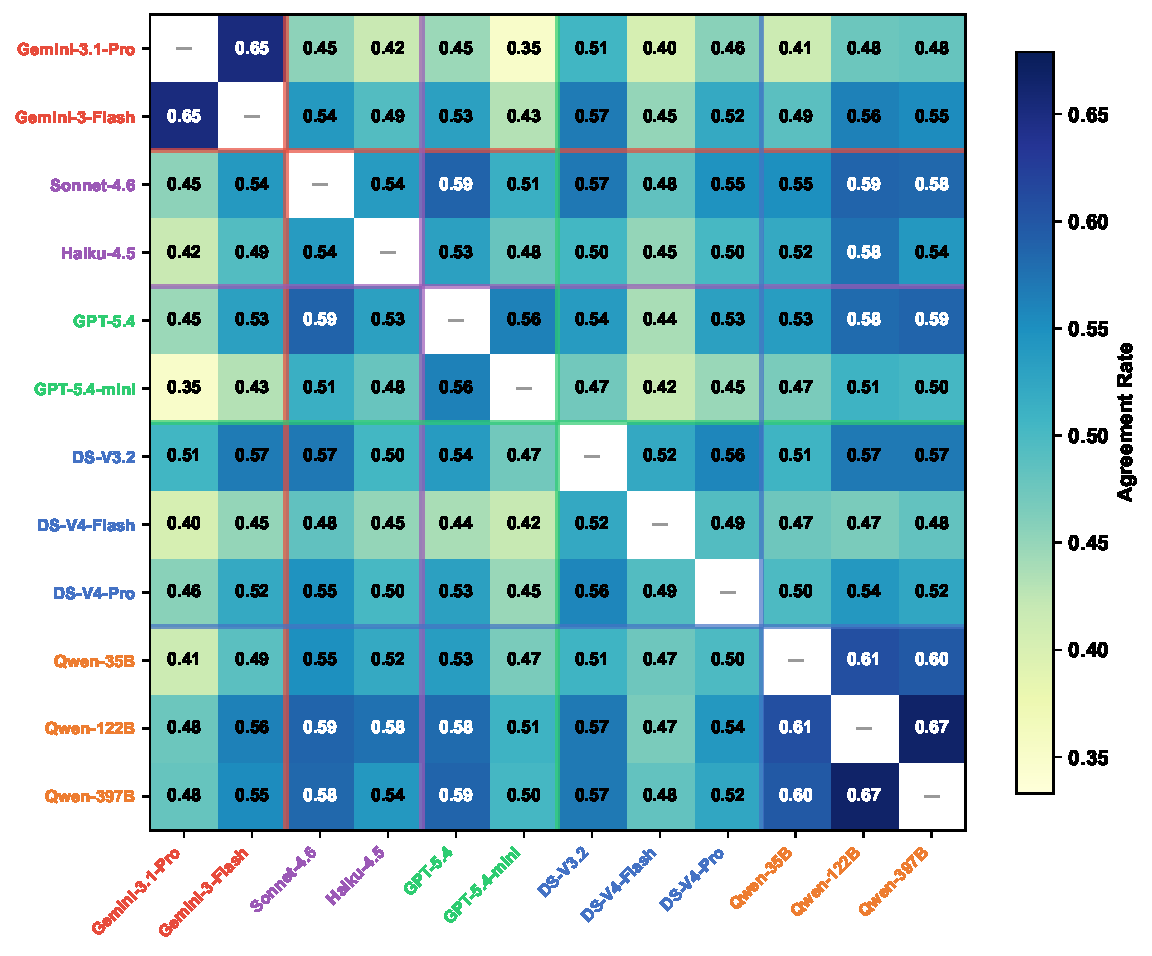
\includegraphics[width=0.75\linewidth]{figures/model_agreement.pdf}
\caption{Pairwise answer agreement rate among 12 models under the Naive-RAG configuration. Diagonal entries are masked. White separator lines delineate model families (Gemini, Claude, GPT, DeepSeek, Qwen).}
\label{fig:model_agreement}
\end{figure}

Figure~\ref{fig:model_agreement} shows that pairwise answer agreement is generally higher within model families than across them. The two Gemini models agree on 65.0\% of questions, and the three Qwen3.5 variants reach up to 66.7\%; the overall cross-model mean is 51.4\%. The lowest reported cross-family pair is Gemini-3.1-Pro and GPT-5.4-mini (35.0\%). Claude-Sonnet-4.6 agrees more often with GPT-5.4 and Qwen3.5-397B (around 58--59\%) than with Claude-Haiku-4.5 (54.0\%). These descriptive patterns show that evaluated models often select different options; they do not by themselves identify the underlying reasoning strategies or their causes.

% ============================================================
\subsection{Age-Defined Life-Stage Performance Analysis}
\label{app:life_stage}
% ============================================================

\begin{figure*}[h]
\centering
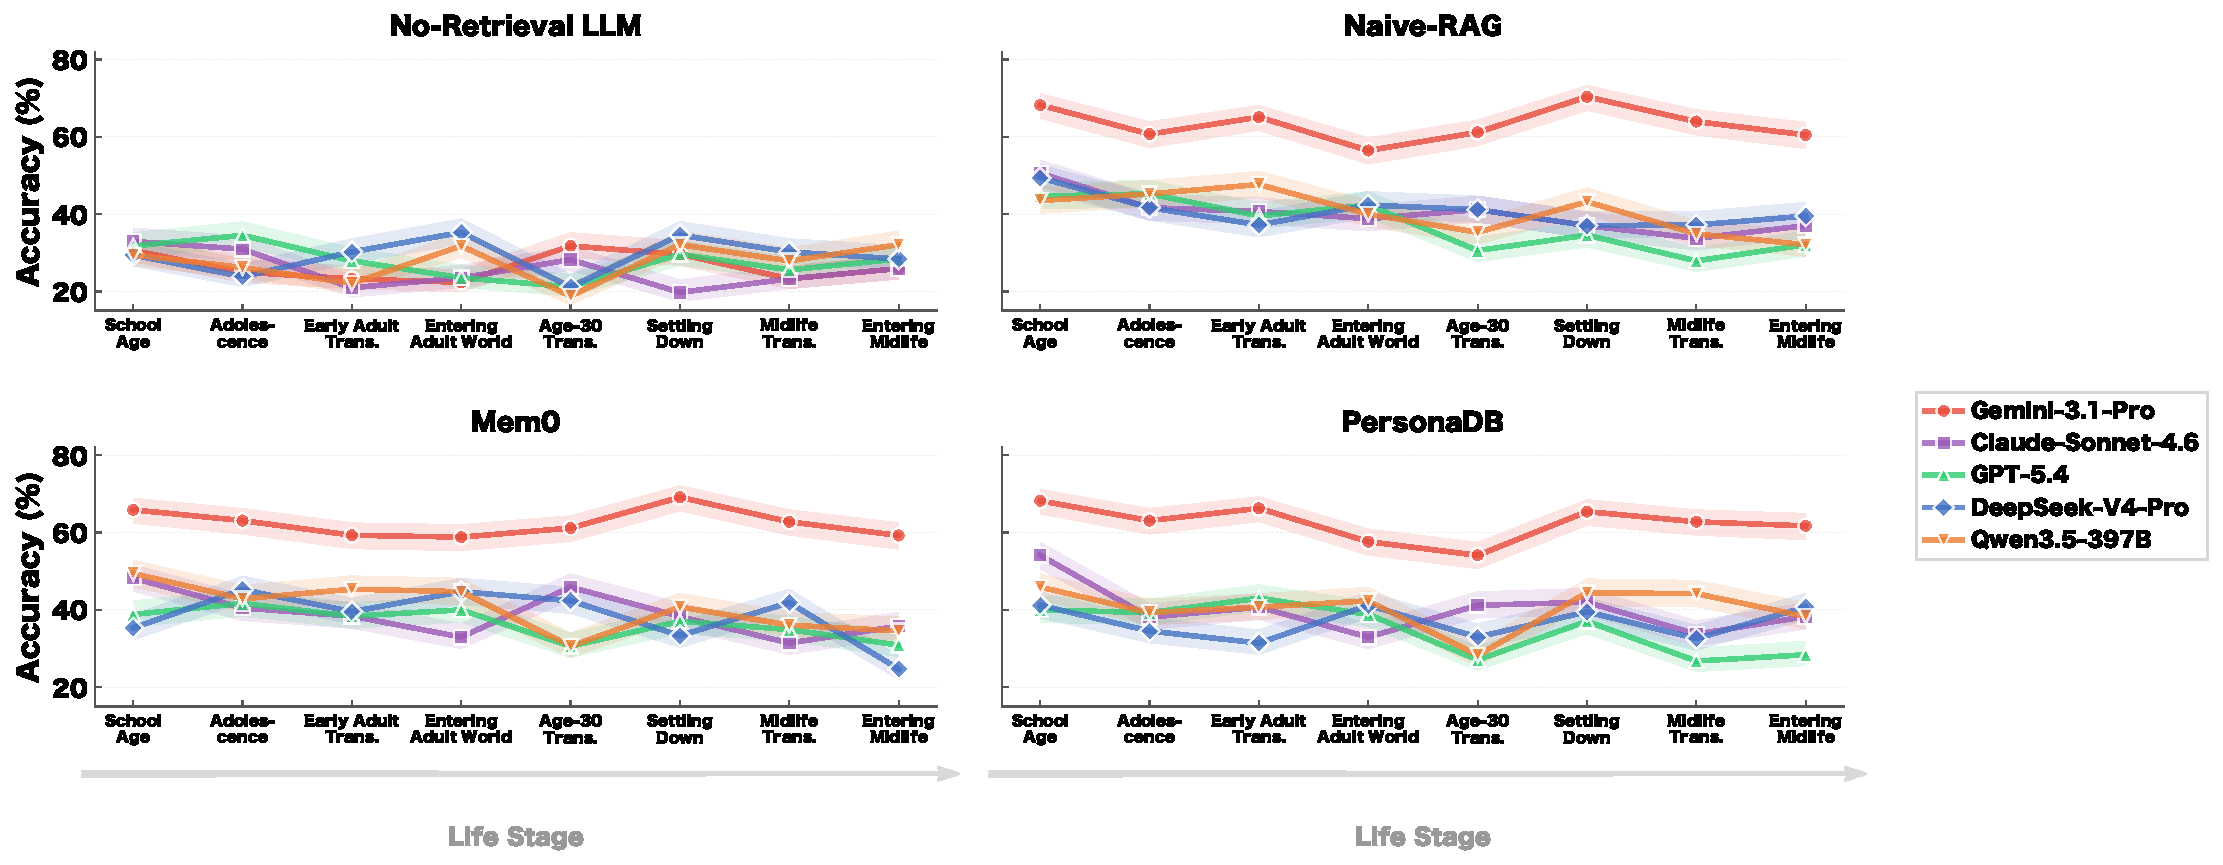
\includegraphics[width=\linewidth, trim=0 10 0 0 clip]{figures/per_stage_accuracy.pdf}
\caption{Accuracy by age-defined life-stage bin across the No-Retrieval baseline and three memory-augmented settings. Each line represents the best-in-family model.}
\label{fig:per_stage}
\end{figure*}

\textbf{Accuracy varies across life-stage bins.} Figure~\ref{fig:per_stage} reports a descriptive breakdown by the benchmark's age-defined bins. Accuracy is highest at School Age (47.1\%) and lower at Age-30 Transition (37.4\%) and Midlife Transition (37.9\%), with Settling Down at 43.1\%. The pattern may reflect differences in designed scenario composition and memory density. Because bins were not randomized and contain different scenarios, it does not support a developmental or causal interpretation. Gemini-3.1-Pro has the highest accuracy in every displayed bin under this benchmark.

\subsection{Character-Level Error Analysis}
\label{app:character_error}

Character-level accuracy in Figure~\ref{fig:per_char_radar} is computed separately for each memory-augmented setting by pooling predictions from all 12 evaluated LLMs within each target character; the values summarized in the main text average these setting-specific accuracies. We define the 221 persistent shared-failure items as MCQs answered incorrectly by all 12 models in each of the three memory-augmented settings. Within this set, Naive-RAG convergence means that at least six of the 12 models select the same non-reference option. We classify a confusion as opposite-pole when the selected option originates from the character anchored at the opposite end of the target character's defining Big Five dimension.

\section{Prompts}
\label{app:prompts}
% ============================================================

This appendix presents the model-facing evaluation template and the system-prompt templates used at each construction stage; long item-specific payloads and embedded exemplars are represented by placeholders for readability. The complete executable prompts are released alongside the benchmark for reproducibility. Construction-time terms such as ``Ground Truth'' are retained verbatim and refer to the benchmark reference response. The evaluated construct remains agreement with expert-adjudicated persona-consistency references.

\subsection{Model Evaluation Prompt}
\label{app:prompt_evaluation}

The evaluation prompt serializes the input in a fixed order: basic character information, retrieved autobiographical memories, the current scenario, the trigger event, the task instruction, and four shuffled response options. The memory block is populated in the three memory-augmented settings and omitted in the No-Retrieval condition. The template below preserves the complete block structure and required JSON output schema; bracketed placeholders replace item-specific content and repeated memory entries. The released implementation contains the exact executable prompt strings.

\begin{tcolorbox}[
  breakable,
  colback=blue!5,
  colframe=blue!60!black,
  title={\textbf{Model Evaluation Prompt Template}},
  fonttitle=\bfseries,
  rounded corners,
  boxrule=1.0pt
]
\begin{Verbatim}[fontsize=\scriptsize, breaklines=true, breaksymbolleft={}, breaksymbolright={}, breakindent=1em]
[SYSTEM]
You are a role-playing simulator. You will receive a person's basic
information, past experiences, current situation, and possible behavioral
decisions. Infer the person's patterns of thought, emotion, and behavior from
the supplied evidence, and select the response that this person would most
likely make. Return only a valid JSON object in the following format:

{
  "system_1_impulse": {
    "thought": "immediate reaction",
    "emotion": "primary emotion",
    "citation": "memories associated with the reaction"
  },
  "system_2_rational": {
    "analysis": "deliberative analysis",
    "plan": "action plan"
  },
  "inner_consciousness": "first-person reason for the decision",
  "final_decision": "first-person behavioral response",
  "decision_choice": "A|B|C|D"
}

[USER]
## Basic character information
Character ID: [CHARACTER_ID]
Occupation: [OCCUPATION]

## Retrieved autobiographical memories
[MEMORY_1]
...
[MEMORY_K]

## Current scenario
Scenario: [SCENARIO_NAME]
Setting: [LOCATION] | [TIME] | [ATMOSPHERE]
Background: [SCENARIO_BACKGROUND]

## Trigger event
Sender: [SENDER]
Message: [MESSAGE_CONTENT]
Required decision: [ACTION_REQUIRED]

## Task
Use the supplied experiences to infer this person's thought patterns,
emotional tendencies, and behavioral habits. Simulate how the person would
respond in the current situation and select the most persona-consistent option.

## Decision options
A. [OPTION_A]
B. [OPTION_B]
C. [OPTION_C]
D. [OPTION_D]

Return the selected letter in the "decision_choice" field.
\end{Verbatim}
\end{tcolorbox}

Only \texttt{decision\_choice} is used to compute benchmark accuracy. The structured rationale fields are requested as part of a common response format, but their content is neither graded nor used to resolve the selected option.

\paragraph{Output parsing and invalid responses.}
Model outputs are parsed for the \texttt{decision\_choice} field and normalized to one of \texttt{A}, \texttt{B}, \texttt{C}, or \texttt{D}. When full JSON parsing fails, the evaluator attempts to recover an explicitly named \texttt{decision\_choice} from the raw response. If no valid option can be recovered, the response is counted as incorrect; refusals receive the same treatment. No answer is inferred from the rationale or \texttt{final\_decision} fields, which are retained only for inspection.

\subsection{Character Generation Prompt}
\label{app:prompt_character}

We use the following prompt with Claude Opus 4.6 to generate the 11 trait-anchored Big Five character profiles, each with a self-value logic and eight core behavioral patterns. It is used once per character to establish the predefined profile artifact before memory generation.

\begin{tcolorbox}[
  breakable,
  colback=blue!5,
  colframe=blue!60!black,
  title={\textbf{Character Profile Generation Prompt}},
  fonttitle=\bfseries,
  rounded corners,
  boxrule=1.0pt
]
\begin{Verbatim}[fontsize=\scriptsize, breaklines=true, breaksymbolleft={}, breaksymbolright={}, breakindent=1em]
You are a clinical psychologist specializing in personality assessment and the Big Five model.
Generate a complete character profile for a virtual human in a personality research project.

## Requirements
1. Big Five scores: Provide exact scores for O, C, E, A, N (0.0-1.0 scale)
2. One dimension must be extreme (0.95 for high or 0.10 for low), others moderate (0.30-0.70)
3. Self-value logic: One sentence describing the character's core cognitive operating principle
4. Core behavioral patterns: Exactly 8 specific, observable patterns that manifest the dominant trait
5. Occupation: Must be ecologically consistent with the dominant trait

## Output Format (JSON)
{
  "char_key": "CHAR_XX",
  "name": "Chinese name",
  "occupation": "specific job title",
  "big_five": {"O": 0.X, "C": 0.X, "E": 0.X, "A": 0.X, "N": 0.X},
  "big_five_str": "O=0.X, C=0.X, E=0.X, A=0.X, N=0.X",
  "description": "2-3 sentence character summary",
  "self_value_logic": "one sentence core principle",
  "core_patterns": [
    "pattern 1: specific observable behavior",
    "pattern 2: ...",
    ...
    "pattern 8: ..."
  ]
}
\end{Verbatim}
\end{tcolorbox}

\subsection{Memory Generation Prompt}
\label{app:prompt_memory}

This prompt generates the 11,000 episodic memories (1,000 per character) spanning ages 6--50. It enforces coverage of Rubin's five dimensions, strict temporal perspective lock, age-stratified language, and the ABCD intensity model.

\begin{tcolorbox}[
  breakable,
  colback=blue!5,
  colframe=blue!60!black,
  title={\textbf{Memory Generation System Prompt (Claude Sonnet 4.6)}},
  fonttitle=\bfseries,
  rounded corners,
  boxrule=1.0pt
]
\begin{Verbatim}[fontsize=\scriptsize, breaklines=true, breaksymbolleft={}, breaksymbolright={}, breakindent=1em]
You are a psychology narrative expert writing episodic memories for virtual characters
in a Big Five personality research project.

## Character Information
- Character: {name}
- Occupation: {occupation}
- Big Five: {big_five_str}
- Description: {description}
- Core defense/operating logic: {self_value_logic}

## Core Behavioral Patterns
{core_patterns}

## Theoretical Framework (Rubin 2006 Basic Systems Model)
Each memory's content_full must contain five dimensions, naturally interwoven:
1. Environmental sensory: visual/auditory/tactile/olfactory details
2. Dialogue reconstruction: at least 1-2 segments of real dialogue (in quotes)
3. Inner monologue: first-person immediate thoughts and emotions
4. Somatic response: heartbeat/sweating/muscle tension and other bodily sensations
5. Aftermath: immediate impact after the event (limited to 24 hours-1 week post-event)

## Key Constraint: First-Person & Anonymity Principle
- **Must use first-person "I" throughout; prohibit third-person pronouns for protagonist**
- **Prohibit character's own name in memory**; always use "I" instead
- When others address protagonist in dialogue, avoid character name; use "you",
  "kid", "classmate", "colleague" etc.

## Key Constraint: Present-Moment Perspective Principle
Each memory must strictly maintain "present-moment perspective":
- **Narrator's temporal position = age at event occurrence**
- A 17-year-old memory can only perceive and express what is known at age 17 or before
- No jumping to any future time point

**Forbidden expressions**:
"years later", "many years later", "later I learned", "later I discovered"
"now thinking back", "now recalling", "until now", "I didn't know then"
"until...only then", "it took...to realize", "walked...before realizing"
"if only I had known", "if I had known earlier"
"I thought at the time" (opposing "now" vs "then")
"from then on", "thereafter" (implying long-term impact)
"the whole thing", "the most...part" (post-hoc evaluative summary)

**Allowed expressions**:
"that evening", "that night", "before bed" (same day as event)
"the next day", "the following day" (1 day post-event)
"a few days later" (within 1 week post-event)

## Age-Stratified Narrative Constraints
- **Childhood (6-12 years)**: Simple, direct language; avoid abstract summaries;
  concrete emotion descriptions
- **Adolescence (13-18 years)**: Some self-reflection, but not over-rationalized;
  maintain confusion and intensity
- **Adulthood (19+ years)**: May have more complex psychological analysis, but still
  maintain present-moment perspective

## Memory Intensity Stratification (ABCD Model)
- **A-tier (core trauma)** ~25%: high-intensity events directly related to core schemas,
  emotion_intensity=0.80-0.90
- **B-tier (main-thread)** ~35%: medium-high intensity events related to personality
  traits, emotion_intensity=0.70-0.85
- **C-tier (daily friction)** ~25%: small conflicts and friction in daily life,
  emotion_intensity=0.60-0.75
- **D-tier (noise memory)** ~15%: ordinary daily memories with lower emotional intensity,
  emotion_intensity=0.55-0.65

## Output Format
Strictly follow this JSON format; return only JSON, no other text:
{
  "id": "memory ID",
  "timeline": "stage (X years old)",
  "context": "15-30 character scene description",
  "content_summary": "20-40 character event summary",
  "content_full": "~2000-4500 character first-person narrative",
  "triggers": ["trigger1", "trigger2", "trigger3", "trigger4"],
  "psych_conclusion": "40-80 char psychological conclusion (cite concepts like
                       schemas, defense mechanisms)",
  "behavior_policy": "30-60 char behavioral guideline",
  "emotion_signature": {
    "primary": "primary emotion (English)",
    "secondary": "secondary emotion (English)",
    "intensity": 0.X
  },
  "relevance_tags": ["tag1", "tag2", "tag3", "tag4"]
}
\end{Verbatim}
\end{tcolorbox}

Each generation call pairs this system prompt with a user prompt specifying target age, life-stage bin, intensity layer (A/B/C/D), and a sliding-window anti-duplication list containing the \texttt{context} field of the most recent 100 generated memories to prevent near-duplicate scenarios within the same age window.

\subsection{Scenario Expansion Prompt}
\label{app:prompt_scenario}

This prompt expands a short scenario sketch (one per life-stage bin $\times$ DIAMONDS dimension, drafted in \texttt{docs/diamonds\_scenario\_design.md}) into a complete scenario JSON object. Appendix~\ref{app:ExampleofScenario} shows the scenario-facing fields, including the metadata, background narrative, and trigger event; the prompt additionally requests assessed Big Five trait pressures, Schwartz value conflicts, and per-dimension annotation references for construction-time annotation. The system prompt embeds the ``Shattered Group Presentation'' instance from Appendix~\ref{app:ExampleofScenario} inline so the model has a concrete shape to imitate; the schema description is reproduced below.

\begin{tcolorbox}[
  breakable,
  colback=blue!5,
  colframe=blue!60!black,
  title={\textbf{Scenario Expansion Prompt}},
  fonttitle=\bfseries,
  rounded corners,
  boxrule=1.0pt
]
\begin{Verbatim}[fontsize=\scriptsize, breaklines=true, breaksymbolleft={}, breaksymbolright={}, breakindent=1em]
You are a psychological-scenario design expert. Your task is to expand a short scenario sketch into a complete, high-quality scenario JSON object.

## Output format

Strictly output a single JSON object (no other text, no markdown code block) with the following structure:

{EXAMPLE_SCENARIO}    <- a complete worked example is embedded here in the actual prompt

## Field specification

1. **id**: SCN_{STAGE}_{N} in upper case, where STAGE is one of SCHOOL_AGE / ADOLESCENCE / EARLY_ADULT_TRANSITION / ENTERING_ADULT_WORLD / AGE_30_TRANSITION / SETTLING_DOWN / MIDLIFE_TRANSITION / ENTERING_MIDLIFE.
2. **stage**: lowercase form of the above.
3. **diamonds_dimension**: the dominant DIAMONDS dimension (Duty, Adversity, Positivity, ...) as given in the sketch.
4. **name**: "Chinese name (English Name)".
5. **category**: two short labels separated by " / ".
6. **intensity**: Low / Medium / High / Very High / Extreme.
7. **description_for_agent**: one sentence summarizing the scenario without revealing concrete details.
8. **setting**: location, time, and 2-3 atmosphere adjectives.
9. **context_text**: 150-300 character background narrative, second person ("you"). **Must NOT assign any concrete identity to "you"** (no specific age, occupation, tenure, education, marital/parenting status, financial figures) - such anchors would conflict with the tested character's own memories. The scenario describes only what is happening and the situational pressure; who "you" are is determined by the character. Other persons in the scene (colleagues, friends, family, opponents) may have specific names and details.
10. **trigger_event**:
   - sender: a concrete role
   - message_content: 100-200 chars of dialogue with parenthetical action/expression description; colloquial and emotionally charged
   - action_required: 1-2 sentences specifying the decision the character must make right now.
11. **assessed_dimensions**:
    - trait_pressures: typically 1-3 entries. Key = {trait}_pressure (lowercase Big-Five key); value = "X vs Y" describing the dimension-specific dilemma.
    - value_conflicts: typically 1-3 entries. Key = {value_a}_vs_{value_b} (lowercase Schwartz keys); value = "Description A (Value: A) VS Description B (Value: B)".
12. **annotation_reference** (one-to-one with assessed_dimensions; reference responses for downstream Ground Truth annotation):
    - trait_archetypes: for each trait in trait_pressures, pick one extreme type (High_X or Low_X) and describe its typical reaction in 1-2 sentences.
    - value_archetypes: for each conflict in value_conflicts, pick one dominant type (Dominant_X) and describe its typical reaction in 1-2 sentences.

## Key principles

1. **Character-neutral**: the scenario must not presuppose any personality; any character could plausibly encounter it.
2. **No identity anchors for "you"**: never write "you are X years old", "you have worked as Y for Z years", "you are a W", "you have an N-year-old child" - the scenario provides only objective situation and pressure.
3. **Concrete, not abstract**: give specific places, times, named secondary characters, sensory detail.
4. **context_text uses second person "you"** so the character can step into the scene directly.
5. **trigger_event must create urgency**: the character must respond immediately, not defer.
6. **Tightly aligned with diamonds_dimension**: background, trigger, and assessed dimensions all center on the dominant DIAMONDS dimension.
7. **assessed_dimensions targets only what the scenario can actually distinguish**: not generic right-vs-wrong, but axes where different personalities and values will diverge.
8. **annotation_reference must one-to-one cover assessed_dimensions**.
9. **Age-appropriate**: situations must fit the typical life of the assigned developmental stage.

## Big Five labels (use exactly these 5 keys)

- Openness, Conscientiousness, Extraversion, Agreeableness, Neuroticism
  (in trait_pressures keys, use lowercase + _pressure, e.g. conscientiousness_pressure)

## Schwartz value labels (use exactly these 19 keys)

Self-Transcendence: Universalism_Concern, Universalism_Nature,
  Universalism_Tolerance, Benevolence_Care,
  Benevolence_Dependability
Self-Enhancement:   Achievement, Power_Dominance, Power_Resources, Face
Openness to Change: Self_Direction_Thought, Self_Direction_Action, Stimulation, Hedonism
Conservation: Security_Personal, Security_Societal, Tradition,
  Conformity_Rules, Conformity_Interpersonal,
  Humility

In value_conflicts keys, use the lowercase underscore form (e.g. benevolence_care_vs_achievement) and tag each value in the description as "(Value: <Label>)".
\end{Verbatim}
\end{tcolorbox}

The user prompt is short and per-draft: it provides the life-stage bin, the dominant DIAMONDS dimension, the draft's short title, and the draft body parsed verbatim from \texttt{diamonds\_scenario\_design.md}, then asks for the full JSON object. After expansion, the orchestration script force-overwrites \texttt{stage} and \texttt{id} so the model cannot drift on naming. Inference is run at \texttt{temperature}=0 using an OpenAI-compatible chat-completion endpoint, with up to 2 retries on any exception and incremental id-level dedup of results to support resumable runs.

\subsection{Annotation Prompts}
\label{app:prompt_annotation}

This section describes benchmark-construction prompts only. None of these prompts or their structured psychological fields is used by the Naive-RAG, Mem0, or PersonaDB evaluation pipeline, for which the sole memory input is \texttt{content\_full}.

The candidate-response construction pipeline runs in three stages, each driven by a dedicated system prompt. Stage~1 performs a permissive binary relevance screen of every memory whose age falls at or before the scenario age; Stage~2 refines the survivors down to a fixed budget (default 50); Stage~3 role-plays the character to produce a first-person rationale and final response. The user prompts for each stage concatenate character information, the current scenario, the (candidate) memory list, and a closing instruction; only the system prompts are reproduced here for brevity.

\subsubsection{Stage 1 --- Memory Activation Screening}
\label{app:prompt_activation}

This prompt is issued once per character $\times$ scenario $\times$ age batch. It enumerates the six retrieval-cue mechanisms (structural similarity, emotional resonance, self-schema, behavioral script, narrative identity, somatic marker) the model should consult, and asks for a JSON array containing only the activated memories.

\begin{tcolorbox}[
  breakable,
  colback=blue!5,
  colframe=blue!60!black,
  title={\textbf{Stage 1 --- Memory Activation Screening Prompt}},
  fonttitle=\bfseries,
  rounded corners,
  boxrule=1.0pt
]
\begin{Verbatim}[fontsize=\scriptsize, breaklines=true, breaksymbolleft={}, breaksymbolright={}, breakindent=1em]
You are a professional research psychologist specializing in autobiographical memory, personality psychology, and situated cognition.

Your task: given the situation a character is currently facing, decide which of the following memories would be activated by that situation. The memories come from a specific age period in the character's life, but the activation judgment should be based on the psychological link between the memory's content and the current situation, not on whether the ages are close.

## Psychological mechanisms of memory activation

Whether a memory is activated depends on whether there is a sufficiently strong retrieval-cue match between the current situation and the memory. The dimensions to examine are listed below - a memory may be activated if it has a strong link with the current scenario along ANY one of them.

### 1. Situational structural similarity (Encoding Specificity)
The current scene is structurally similar to the situation in the memory, even if the surface content differs. Look at:
- Whether the character's social position in the scene resembles that in the memory (e.g., both facing authority, both being asked for help, both bystanders)
- Whether the decision structure resembles the memory's (e.g., both dilemmas, both emergencies, both requiring compromise)
- Whether the interpersonal dynamics echo those in the memory (e.g., trust-betrayal, competition-cooperation, intimacy-distance)

### 2. Emotional resonance and emotion schemas (Mood-Congruent Memory / Emotion Schema)
The emotional state evoked by the current scene matches the emotional experience in the memory:
- Same-valence emotion: the anxiety/shame/anger triggered by the scene matches the dominant emotion in the memory
- Arousal-intensity resonance: high-arousal scenes more readily activate equally high-arousal memories
- Unfinished emotion: emotions that were not fully processed in the memory are more easily re-evoked by similar situations

### 3. Self-schema and core-belief activation (Self-Schema / Core Belief Activation)
The core beliefs formed in the memory (psych_conclusion) relate to the self-cognition the current scene touches:
- Whether the scene challenges or confirms the self-cognition formed in the memory
- Whether the scene touches a relational schema established by the memory
- Whether the scene evokes a worldview assumption from the memory

### 4. Behavioral scripts and procedural links (Behavioral Script)
The behavior_policy formed in the memory can serve directly as an action template for the current scene:
- Whether the memory's behavioral strategy applies to the current decision
- Whether the character has formed habitual response patterns in similar situations before
- Including avoidance: if the memory's outcome was painful, the character may be inclined toward the opposite action

### 5. Narrative identity and life themes (Narrative Identity)
The memory is a key node in the character's self-narrative:
- Turning-point memories: events that mark a change in life direction
- Origin-story memories: events the character uses to explain "why I am the way I am"
- Recurring themes: patterns that keep appearing in the character's life

### 6. Somatic markers and sensory cues (Somatic Marker)
Sensory elements in the current scene have a direct link to sensory experiences in the memory:
- Similar physical environments, similar bodily sensations, or specific sensory triggers (e.g., the sound of arguing, a particular smell or season)

## Important notes

- Don't only look at "topic relevance" - deep psychological links matter more than surface similarity.
- Memories from early development that formed core beliefs or emotional patterns can still be readily activated by later scenes.
- High-emotional-intensity memories (trauma, major successes, deep interpersonal connections) have lower activation thresholds.

## Output format

Strictly output a JSON array (no markdown code block), containing ONLY the activated memories:

[
  {
    "memory_id": "MEM_XX_XXXX",
    "reason": "20-30 chars, indicating which mechanism activated it."
  }
]

If no memory in this batch is activated, output an empty array [].

## Cautions

- Output only the activated memories; do not output non-activated ones.
- A reference activation count is given at the end of each batch - treat it as an UPPER bound; prefer fewer over more. Only memories with a STRONG, DIRECT psychological link to the current situation should be selected.
- Do not invent memory_id values not in the list.
\end{Verbatim}
\end{tcolorbox}

The accompanying user prompt concatenates four blocks: character info, the candidate-memory list for the age window, the current scenario (background and trigger event), and a closing instruction quoting a per-batch activation budget derived from \texttt{TARGET\_ACTIVATED}=50 and an upstream buffer ratio of 1.5. Inference is run at \texttt{temperature}=0 with up to two retries on JSON-parse failures.

\subsubsection{Stage 2 --- Activated-Memory Refinement}
\label{app:prompt_finalize}

Stage 2 takes the union of Stage-1 activations and reduces it to at most the target count (default 50) per scenario. The prompt enforces a three-tier priority (behavior-driving, frame-shaping, emotion-supplying) and a de-redundancy rule that prefers the earliest schema-forming instance among psychologically equivalent memories. When the candidate count is already at or below the target, Stage 2 is skipped without an LLM call.

\begin{tcolorbox}[
  breakable,
  colback=blue!5,
  colframe=blue!60!black,
  title={\textbf{Stage 2 --- Activated-Memory Refinement Prompt}},
  fonttitle=\bfseries,
  rounded corners,
  boxrule=1.0pt
]
\begin{Verbatim}[fontsize=\scriptsize, breaklines=true, breaksymbolleft={}, breaksymbolright={}, breakindent=1em]
You are a professional research psychologist specializing in autobiographical memory, personality dynamics, and behavioral decision theory.

Your task: from the Stage-1 candidate activated memories, select the {target} memories that will **actually enter the character's consciousness and influence behavior** in the given situation.

## Psychological basis for refinement

Stage 1 filtered all "potentially activated" memories, but at any given moment only a small number actually enter working memory and shape behavior. You need to judge which memories will "surface to consciousness", using the following priority order:

### Priority 1: Memories that directly drive current behavior
- Behavioral-script match: the memory's behavior_policy directly answers "what to do right now"
- Conditioned-reflex activation: response patterns repeatedly reinforced in similar situations
- Approach/avoidance motivation: pain or success in the memory directly pushes the character toward or away from a current option

### Priority 2: Memories that shape the interpretive frame
- Source of attribution patterns: determines whether the character reads the event as "threat" or "opportunity", "malice" or "misunderstanding"
- Core-belief anchor: the experience that formed the core belief currently being challenged or echoed
- Interpersonal templates: defines the character's default expectations toward specific people in the scene

### Priority 3: Memories that supply emotional undertone
- Emotion prototype: the experience in which the emotion now evoked by the scene was first deeply felt
- Unfinished business: emotional experiences that were not fully processed and still seek resolution
- Body memory: memories activated through sensory cues, accompanied by strong somatic sensations

### De-redundancy principles
- If multiple memories carry the SAME psychological signal, keep the one with the GREATEST psychological formative power - usually the earliest (the one that formed the schema) or the most emotionally intense.
- Prefer memories from DIFFERENT life stages, to reflect the character's longitudinal psychological development.
- Deep linkage outweighs surface topical similarity.

## Output format

Strictly output a JSON object (no markdown code block):

{
  "activated_memories": [
    {
      "memory_id": "MEM_XX_XXXX",
      "type": "BS|AM|CB|ER|DL|NI",
      "reason": "20-30 chars"
    }
  ]
}

Type codes: BS=behavioral script, AM=attribution mode, CB=core belief, ER=emotional resonance, DL=deep linkage, NI=narrative identity.
The array order is the ranking (item 1 = most influential).

## Cautions

- Output exactly {target} entries - no more, no fewer.
- Do not invent memory_id values not in the candidate list.
\end{Verbatim}
\end{tcolorbox}

The user prompt provides character info, the current scenario, and the candidate list (each entry annotated with its Stage-1 activation reason). Inference is run at \texttt{temperature}=0 with reasoning explicitly disabled.

\subsubsection{Stage 3 --- Candidate Response Generation}
\label{app:prompt_gt}

The final stage role-plays the character in first person and produces a structured candidate: a first-person rationale, an emotional-tone description, character-specific reasoning, value orientation, and a two-sentence \texttt{final\_decision}. This output becomes one of three candidates reviewed by experts; it does not itself define the benchmark label. The prompt forbids psychological terminology and memory-ID enumeration, asking the model to incorporate retrieved content as associations rather than citations.

\begin{tcolorbox}[
  breakable,
  colback=blue!5,
  colframe=blue!60!black,
  title={\textbf{Stage 3 --- Candidate Response Generation Prompt}},
  fonttitle=\bfseries,
  rounded corners,
  boxrule=1.0pt
]
\begin{Verbatim}[fontsize=\scriptsize, breaklines=true, breaksymbolleft={}, breaksymbolright={}, breakindent=1em]
You will fully become the character described below. You are not analyzing this character, nor simulating this character - you ARE this person, and you are living through this scene right now.

You will be given:
1. **Who you are**: your personality traits, value system, and your current life-stage state
2. **What you are going through**: the current scenario and the trigger event
3. **Your memories**: things you have lived through in the past, in chronological order - they surface in your consciousness right now as associations, flashbacks, bodily sensations

## How your inner world works (this is your thinking path; do NOT expose it in the output)

Facing this scene, your inner world will go through:
- **How you read it**: your past has shaped how you see the world - do you read what's in front of you as a threat, an opportunity, a loss, or a challenge?
- **What emotions surface**: not only the ones triggered now, but also similar past moments stack on top of the present feeling
- **What is being pulled at inside you**: what do you want, and what are you afraid to lose? Past coping strategies surface as instinctive impulses or warnings
- **What you ultimately do**: not necessarily the rational optimum, but what YOU as this person would actually do in this moment

## Output format

Strictly output a JSON object (no markdown code block):

{
  "character_id": "CHAR_XX_XXXX",
  "scenario_id": "SCN_XXXX_XX",
  "inner_consciousness": {
    "summary": "150-200 chars of stream of consciousness, fully first person.",
    "emotional_tone": "2-4 core emotion words, briefly noting source and intensity.",
    "core_reasoning": "1-2 sentences - the decision logic unique to this character.",
    "value_orientation": "1-2 sentences, in the character's own inner voice."
  },
  "final_decision": "Two sentences, ~50 chars total. First summarizes the choice; second writes the concrete action."
}

## Must follow

1. **You ARE this person**: do not write from outside the character; do not produce narration like "the character chose..." "they decided..."
2. **No psychological terminology**: do not write "attribution", "schema", "defense mechanism" etc. - only plain human language
3. **Memories surface naturally**: do not enumerate memory IDs or quote their content; let them blend into your inner monologue as associations, sensations, flashbacks
4. **Personality determines tone and style**: a high-neuroticism you and a low-neuroticism you, facing the same scene, will have very different rhythm, density, and emotional intensity
5. **Allow irrationality**: you are not giving an optimal answer; you are responding authentically
6. **Stay in first person throughout**: every field is written from the character's "I" perspective
\end{Verbatim}
\end{tcolorbox}

The user prompt for Stage 3 supplies the full character snapshot (Big Five, dominant/suppressed Schwartz values, self-value logic, semantic memory, and life-stage-bin snapshot), the scenario (background, trigger event, action required, assessed personality/value dimensions), and the chronologically sorted Stage-2 activated memories with their \texttt{psych\_conclusion}, \texttt{behavior\_policy}, and emotion signature.

\end{document}
